%================================================================
% RAPPORT DE STAGE / PROJET DE FIN D'ETUDES
% KODA — Assistant de Vie (Ami Virtuel) — Système Embarqué Intelligent
% Classe DSI3.2 — ISET Mahdia
%================================================================

\documentclass[a4paper,12pt]{report}

%----------------------------------------------------------------
% Encodage & langue
%----------------------------------------------------------------
\usepackage[T1]{fontenc}
\usepackage[utf8]{inputenc}
\usepackage[english,french]{babel} 


%----------------------------------------------------------------
% Police Times New Roman
%----------------------------------------------------------------
\usepackage{mathptmx}            % Times New Roman pour texte et maths
\usepackage{amssymb}             % \checkmark, etc.

%----------------------------------------------------------------
% Mise en page
%----------------------------------------------------------------
\usepackage[
a4paper,
top=2cm,
bottom=2cm,
left=2.5cm,   % 2cm + 0.5cm reliure
right=2cm,
headheight=14pt
]{geometry}

\usepackage{setspace}
\setstretch{1.5}                 % Interligne 1.5

\usepackage{microtype}           % Meilleure justification
\usepackage{ragged2e}

%----------------------------------------------------------------
% Couleurs & graphiques
%----------------------------------------------------------------
\usepackage{xcolor}
\usepackage{graphicx}
% Pas de flottants pour les figures KODA (\kodafigure) ; \FloatBarrier = no-op sans placeins
\newcommand{\FloatBarrier}{}

\makeatletter
\newcommand{\nonfloatingfigure}[3]{%
  \vspace{\intextsep}
  \begin{center}
    \makebox[\textwidth][c]{\includegraphics[width=0.9\textwidth]{#1}}
    \def\@captype{figure}
    \caption{#2}
    \label{#3}
  \end{center}
  \vspace{\intextsep}
}
\makeatother

% Figure non flottante (reste sous le titre de section ; label optionnel via 4e argument)
\makeatletter
\newcommand{\kodafigure}[3][0.98\textwidth]{%
  \par\vspace{0.5em}%
  \begin{center}%
    \includegraphics[width=#1]{#2}%
    \captionof{figure}{#3}%
  \end{center}%
  \vspace{0.5em}%
}
\newcommand{\kodafigureL}[4][0.98\textwidth]{%
  \kodafigure[#1]{#2}{#3}%
  \label{#4}%
}
\makeatother
\usepackage{tikz}
\usepackage{pgfgantt}
\usetikzlibrary{shapes.geometric, arrows.meta, positioning, backgrounds}

\definecolor{BleuPrimaire}{HTML}{185FA5}
\definecolor{BleuClair}{HTML}{D6E8F8}
\definecolor{VertPrimaire}{HTML}{3B6D11}
\definecolor{VertClair}{HTML}{D6ECC2}
\definecolor{VioletPrimaire}{HTML}{534AB7}
\definecolor{VioletClair}{HTML}{E0DFFA}
\definecolor{CoralPrimaire}{HTML}{993C1D}
\definecolor{CoralClair}{HTML}{F5D5C8}
\definecolor{GrisFonce}{HTML}{2C2C2A}
\definecolor{GrisMoyen}{HTML}{5F5E5A}
\definecolor{GrisClair}{HTML}{F1EFE8}
\definecolor{AmbreJaune}{HTML}{BA7517}
\definecolor{AmbreClair}{HTML}{FAEEDA}

%----------------------------------------------------------------
% Tableaux
%----------------------------------------------------------------
\usepackage{array}
\usepackage{tabularx}
\usepackage{booktabs}
\usepackage{longtable}
\usepackage{multirow}
\usepackage{colortbl}
\usepackage{makecell}

%----------------------------------------------------------------
% Listes
%----------------------------------------------------------------
\usepackage{enumitem}
\setlist[itemize]{label=\textbullet, leftmargin=1.5em, itemsep=2pt, topsep=4pt}
\setlist[enumerate]{leftmargin=1.5em, itemsep=2pt, topsep=4pt}

%----------------------------------------------------------------
% En-tetes et pieds de page (fancyhdr)
%----------------------------------------------------------------
\usepackage{fancyhdr}
\usepackage{emptypage}           % Pas d'en-tete sur pages vides

% Style par defaut (chapitres)
\fancypagestyle{mainStyle}{
	\fancyhf{}
	\fancyhead[L]{\small\textit{\leftmark}}
	\fancyhead[R]{}
	\fancyfoot[L]{\small KODA --- Accompagnateur de vie, amie virtuelle KODA --- Système Embarqué Intelligent}
	\fancyfoot[R]{\small\thepage}
	\renewcommand{\headrulewidth}{0.4pt}
	\renewcommand{\footrulewidth}{0.4pt}
}

% Style pages pre-liminaires (pas de numero)
\fancypagestyle{preStyle}{
	\fancyhf{}
	\renewcommand{\headrulewidth}{0pt}
	\renewcommand{\footrulewidth}{0pt}
}

%----------------------------------------------------------------
% Titres de chapitres et sections (Times, tailles conformes)
%----------------------------------------------------------------
\usepackage{titlesec}
\usepackage{titletoc}

% Format for numbered chapters (isolated page with rules)
\titleformat{\chapter}[display]
{\null\vspace*{\fill}\centering\normalfont}
{\rule{3cm}{2.5pt}\quad\fontsize{20}{24}\bfseries\MakeUppercase{\chaptertitlename}~\thechapter\quad\rule{3cm}{2.5pt}}{20pt}
{\fontsize{18}{22}\bfseries\MakeUppercase}
[\vspace*{\fill}\clearpage]

% Format for unnumbered chapters (Introduction Générale, Conclusion Générale)
\titleformat{name=\chapter,numberless}[display]
{\null\vspace*{\fill}\centering\normalfont}
{}{0pt}
{\fontsize{22}{26}\bfseries\MakeUppercase}
[\vspace*{\fill}\clearpage]

\titlespacing*{\chapter}{0pt}{0pt}{0pt}
\titlespacing*{name=\chapter,numberless}{0pt}{0pt}{0pt}

% Section : Titre 2 => taille 14, gras
\titleformat{\section}
{\normalfont\fontsize{14}{17}\bfseries}
{\thesection}{0.8em}{}
\titlespacing*{\section}{0pt}{16pt}{8pt}

% Subsection : Titre 3 => taille 12, gras
\titleformat{\subsection}
{\normalfont\fontsize{12}{15}\bfseries}
{\thesubsection}{0.8em}{}
\titlespacing*{\subsection}{0pt}{12pt}{6pt}

% Subsubsection : Titre 4 => taille 12, gras italique
\titleformat{\subsubsection}
{\normalfont\fontsize{12}{15}\bfseries\itshape}
{\thesubsubsection}{0.8em}{}
\titlespacing*{\subsubsection}{0pt}{10pt}{4pt}

%----------------------------------------------------------------
% Figures et tableaux
%----------------------------------------------------------------
\usepackage{caption}
\captionsetup[figure]{
	font=small,         % taille 10
	labelfont=bf,
	position=below,
	skip=4pt
}
\captionsetup[table]{
	font=small,         % taille 10
	labelfont=bf,
	position=above,
	skip=4pt
}

%----------------------------------------------------------------
% Boites colorees (tcolorbox)
%----------------------------------------------------------------
\usepackage{tcolorbox}
\tcbuselibrary{skins, breakable}

\newtcolorbox{ucbox}[1]{
	enhanced, breakable,
	colback=#1!8, colframe=#1,
	arc=4pt, boxrule=0.6pt,
	left=8pt, right=8pt, top=5pt, bottom=5pt
}

\newtcolorbox{sprintbox}[2][]{
	enhanced, breakable,
	colback=#2!10, colframe=#2,
	arc=6pt, boxrule=0.7pt,
	left=10pt, right=10pt, top=8pt, bottom=8pt,
	fonttitle=\bfseries\small\color{white},
	title=#1,
	attach boxed title to top left={yshift=-2mm, xshift=6mm},
	boxed title style={colback=#2, arc=3pt, boxrule=0pt}
}

%----------------------------------------------------------------
% Hyperliens
%----------------------------------------------------------------
\usepackage[hidelinks]{hyperref}
\hypersetup{
	pdfauthor={Oussema Karia \& Salahedin Jendoubi},
	pdftitle={Rapport PFE --- Koda --- Robot compagnon intelligent et émotionnel connecté, piloté par une application cross-plateforme },
	pdfsubject={Projet de Fin d'Etudes}
}

%----------------------------------------------------------------
% Commandes utilitaires
%----------------------------------------------------------------
\newcommand{\badge}[2]{%
	\colorbox{#1}{\textcolor{white}{\footnotesize\bfseries\ #2\ }}%
}

% Astuce : empecher les titres en fin de page
\usepackage{needspace}
\newcommand{\sectiontitle}[1]{\needspace{4\baselineskip}\section{#1}}
\newcommand{\subsectiontitle}[1]{\needspace{3\baselineskip}\subsection{#1}}

%----------------------------------------------------------------
% Compteur de pages
%----------------------------------------------------------------
\usepackage{ifthen}

%================================================================
%----------------------------------------------------------------
% Custom Numbering System
%----------------------------------------------------------------
\renewcommand{\thechapter}{\Roman{chapter}}
\renewcommand{\thesection}{\thechapter.\arabic{section}}
\renewcommand{\thesubsection}{\thesection.\arabic{subsection}}
\renewcommand{\thesubsubsection}{\thesubsection.\arabic{subsubsection}}
\renewcommand{\theparagraph}{\thesubsubsection.\arabic{paragraph}}
\renewcommand{\thesubparagraph}{\theparagraph.\arabic{subparagraph}}

\titleformat{\paragraph}[hang]{\normalfont\normalsize\bfseries}{\theparagraph}{1em}{}
\titlespacing*{\paragraph}{0pt}{3.25ex plus 1ex minus .2ex}{0.5em}

\titleformat{\subparagraph}[hang]{\normalfont\small\bfseries}{\thesubparagraph}{1em}{}
\titlespacing*{\subparagraph}{0pt}{2.5ex plus 1ex minus .2ex}{0.5em}

\setcounter{secnumdepth}{5}
\setcounter{tocdepth}{5}
\begin{document}
	
	\selectlanguage{french}
	%================================================================
	
	%----------------------------------------------------------------
	% PAGES PRE-LIMINAIRES (pas de numerotation visible)
	%----------------------------------------------------------------
	\pagestyle{preStyle}
	\pagenumbering{roman}

	
	%================================================================
	%  PAGE DE GARDE
	%================================================================
	\begin{titlepage}
		\begin{center}
			\begin{minipage}[c]{0.45\textwidth}
				\raggedright
				
\includegraphics[height=3.5cm]{public/isetlogo (2).png}
			\end{minipage}%
			\hfill
			\begin{minipage}[c]{0.45\textwidth}
				\raggedleft
				
\includegraphics[height=3.5cm]{public/logos.png}
			\end{minipage}
			
			\vspace{1.5cm}
			{\fontsize{14}{17}\selectfont\textbf{Institut Supérieur des Études Technologiques de Mahdia}}\\[0.3cm]
			{\fontsize{12}{15}\selectfont\textbf{Département : Technologies de l'Informatique}}\\[0.3cm]
			{\fontsize{12}{15}\selectfont\textbf{Développement des Systèmes Informatiques --- DSI3.2}}\\[1.5cm]
			
			\rule{\linewidth}{0.6pt} \\[1cm]
			{\fontsize{22}{26}\selectfont\textbf{Rapport de Projet de Fin d'Études}}\\[0.8cm]
			\rule{\linewidth}{0.6pt} \\[2cm]
			
			{\fontsize{18}{22}\selectfont\textbf{Koda --- Robot compagnon intelligent et émotionnel connecté, piloté par une application cross-platform } }\\[0.4cm]
			{\fontsize{14}{17}\selectfont\textbf{Système Embarqué · Intelligence Artificielle · Application Mobile Cross-Plateforme}}\\[2.5cm]
			
			\begin{minipage}[t]{0.45\textwidth}
				\begin{flushleft}
					\textbf{Réalisé par :}\\[0.2cm]
					Oussema KARIA\\[0.1cm]
					Salahedin JENDOUBI
				\end{flushleft}
			\end{minipage}
			\hfill
			\begin{minipage}[t]{0.45\textwidth}
				\begin{flushright}
					\textbf{Encadré par :}\\[0.2cm]
					M.Wahid BANOUR --- (Encadrant)\\[0.1cm]
					M.Hamza SASSI (Encadrant Entreprise)
				\end{flushright}
			\end{minipage}
			
			\vfill
			
			{\fontsize{12}{15}\selectfont\textbf{Organisme d'accueil :} ---}\\[0.4cm]
			{\fontsize{12}{15}\selectfont\textbf{Période :} Février 2026 -- Juin 2026}\\[0.4cm]
			
			\vspace*{0.5cm}
		\end{center}
	\end{titlepage}
	
	%================================================================
	%  RESUME (VERSO COUVERTURE)
	%  NB : \end{titlepage} inclut déjà un saut de page ; éviter \clearpage ici
	%      (sinon risque de page blanche avant le résumé).
	%================================================================
	\thispagestyle{preStyle}
	
	\vspace{1cm}
	\selectlanguage{french}
	\begin{center}
		{\fontsize{14}{17}\selectfont\bfseries Résumé}
	\end{center}
	
	\noindent
	Ce rapport présente KODA, un système embarqué intelligent conçu pour être un assistant de vie et un ami virtuel doté de sa propre personnalité et nature. KODA est capable de répondre de manière réfléchie à n'importe quelle personne, de raisonner comme un être humain et de reconnaître les individus grâce à ses modes de sécurité et de configuration.
	
	L'architecture du système repose sur plusieurs composants complémentaires : un système embarqué Raspberry Pi constituant le c\oe{}ur physique du robot ; un moteur de workflows n8n formant le cerveau de KODA, responsable de la préparation et de la réflexion des réponses ; une couche de services Python agissant comme distributeur universel, assurant la communication entre n8n, la base de données, l'application mobile et le Raspberry Pi tout en exposant les endpoints de tout l'écosystème ; une application mobile cross-plateforme pour la configuration et le suivi de vie du robot ; et une base de données persistante servant de mémoire à KODA.
	
	\vspace{0.5cm}
	\noindent\textbf{Mots-clés :} Système Embarqué, Assistant Virtuel, Raspberry Pi, n8n, Python, Cross-Plateforme, Intelligence Artificielle, Assistant de Vie, KODA.
	\selectlanguage{french}
	
	%================================================================
	%  DEDICACE - OUSSEMA KARIA
	%================================================================
	\clearpage
	\thispagestyle{preStyle}
	
	\null\vspace*{\fill}
	\begin{center}
		{\fontsize{26}{30}\selectfont\bfseries DÉDICACE}\\[1cm]
		\rule{0.5\textwidth}{0.5pt}\\[1.5cm]
	\end{center}
	
	\begin{flushright}
		\itshape
		Je dédie ce travail à ma famille, pilier silencieux de ma force et source inépuisable de soutien. Merci pour vos sacrifices immenses et pour avoir cru en moi tout au long de mon parcours académique.\\[0.5cm]
		
		À mes parents, pour leur amour inconditionnel, leurs encouragements et leurs prières qui ont été la lumière guidant chacun de mes pas. Ce succès est le vôtre autant que le mien.\\[0.5cm]
		
		À mes amis et collègues, pour leur soutien moral et pour avoir partagé avec moi cette aventure inoubliable.\\[0.5cm]
		
		À mon binôme Salahedin, pour sa persévérance, sa créativité et sa complicité tout au long de ce projet.\\[0.5cm]
		
		À tous ceux qui ont contribué, même par un simple mot d'encouragement, à l'accomplissement de ce travail.\\[0.8cm]
		
		\textbf{\Large Oussema KARIA}
	\end{flushright}
	
	\vspace*{\fill}
	
	%================================================================
	%  DEDICACE - SALAHEDIN JENDOUBI
	%================================================================
	\clearpage
	\thispagestyle{preStyle}
	
	\null\vspace*{\fill}
	\begin{center}
		{\fontsize{26}{30}\selectfont\bfseries DÉDICACE}\\[1cm]
		\rule{0.5\textwidth}{0.5pt}\\[1.5cm]
	\end{center}
	
	\begin{flushright}
		\itshape
		À ma famille,\\
		pour son soutien inconditionnel et ses sacrifices immenses\\
		tout au long de mon parcours académique.\\[0.5cm]
		
		À mon binôme Oussema, pour son enthousiasme, sa rigueur\\
		et sa précieuse collaboration dans la réalisation de ce projet.\\[0.5cm]
		
		À mes encadrants,\\
		pour leur guidance, leur patience et leur expertise technique.\\[0.5cm]
		
		\textbf{\Large Salahedin JENDOUBI}
	\end{flushright}
	
	\vspace*{\fill}
	
	%================================================================
	%  REMERCIEMENTS
	%================================================================
	\clearpage
	\thispagestyle{preStyle}
	\begin{center}
		{\fontsize{16}{20}\selectfont\bfseries Remerciements}
	\end{center}
	\vspace{1em}
	
	\begingroup
	\setlength{\parindent}{0pt}
	\setlength{\parskip}{0.9em}
	
	\textbf{À notre encadrant académique, M.~Wahid Banour,}\\
	nous adressons nos remerciements les plus sincères pour la qualité de l'accompagnement
	pédagogique, la disponibilité dont il a fait preuve à chaque étape, ainsi que pour ses
	conseils exigeants qui ont permis de structurer notre démarche et de renforcer la
	rigueur scientifique et technique de ce travail.
	
	\textbf{À notre encadrant en entreprise, M.~Hamza Sassi,}\\
	nous exprimons toute notre gratitude pour l'accueil au sein de l'organisme d'accueil,
	pour le temps accordé aux échanges techniques et pour les orientations concrètes qui
	ont éclairé nos choix d'architecture et d'intégration tout au long du projet.
	
	\textbf{À la direction et à l'ensemble du corps enseignant de l'ISET de Mahdia,}\\
	et en particulier au département \textit{Développement des systèmes informatiques} (DSI),
	nous témoignons notre reconnaissance pour la formation dispensée, pour l'exigence
	professionnelle transmise et pour l'environnement d'apprentissage qui a rendu possible
	la réalisation de ce projet de fin d'études.
	
	\textbf{À nos proches, amis et camarades,}\\
	nous disons merci pour la patience, les encouragements et la confiance manifestés
	durant cette période intensive ; leur soutien moral a compté autant que le travail
	collectif mené au sein du binôme.
	
	\vspace{1.2em}
	\noindent
	Nous saluons enfin toute personne ayant contribué, directement ou indirectement,
	à l'aboutissement de ce rapport.\\[2em]
	
	\begin{minipage}[t]{0.48\textwidth}
		\raggedright
		\textbf{Oussema Karia}
	\end{minipage}%
	\hfill
	\begin{minipage}[t]{0.48\textwidth}
		\raggedleft
		\textbf{Salahedin Jendoubi}
	\end{minipage}
	\endgroup
	
	%================================================================
	%  Temporarily switch to inline chapter title for TOC/LOF/LOT
	%  (title appears on same page as content, not isolated)
	%================================================================
	\titleformat{name=\chapter,numberless}
	{\normalfont\fontsize{16}{20}\bfseries\centering}{}{0pt}{\MakeUppercase}
	\titlespacing*{name=\chapter,numberless}{0pt}{30pt}{20pt}
	
	%================================================================
	%  TABLE DES MATIERES
	%================================================================
	\clearpage
	\thispagestyle{preStyle}
	\selectlanguage{french}
	\renewcommand{\contentsname}{Sommaire}
	\renewcommand{\listfigurename}{Liste des figures}
	\renewcommand{\listtablename}{Liste des tableaux}
	\tableofcontents
	
	%================================================================
	%  LISTE DES FIGURES
	%================================================================
	\clearpage
	\thispagestyle{preStyle}
	\listoffigures
	
	%================================================================
	%  LISTE DES TABLEAUX
	%================================================================
	\clearpage
	\thispagestyle{preStyle}
	\listoftables
	
	%================================================================
	%  DEBUT DE LA NUMEROTATION ARABE (depuis Introduction Generale)
	%================================================================
	\clearpage
	\pagestyle{mainStyle}
	\pagenumbering{arabic}
	\setcounter{page}{1}
	
	%================================================================
	%  INTRODUCTION GENERALE (unnumbered, isolated title page)
	%================================================================
	\chapter*{Introduction Générale}
	\addcontentsline{toc}{chapter}{Introduction Générale}
	\markboth{Introduction Générale}{Introduction Générale}
	
	Dans un monde en constante évolution technologique, la demande en solutions intelligentes capables d'améliorer la qualité de vie des individus n'a jamais été aussi forte. Les assistants virtuels et les systèmes embarqués intelligents représentent aujourd'hui une réponse concrète à ce besoin, en combinant les avancées de l'intelligence artificielle, des systèmes embarqués et du développement logiciel moderne.
	
	Ce projet de fin d'études, réalisé dans le cadre de la formation en Développement des Systèmes Informatiques (DSI3.2) à l'ISET Mahdia, porte sur la conception et le développement de \textbf{KODA} : un assistant de vie et ami virtuel embarqué. KODA est un système robotique doté de sa propre personnalité et nature, capable de répondre intelligemment à toute personne, de raisonner à la manière d'un être humain, de reconnaître les individus à travers ses modes de sécurité, et d'être configuré et suivi via une application mobile cross-plateforme dédiée.
	
	La problématique centrale de ce projet est : \textbf{Comment concevoir un système embarqué intelligent capable d'assurer un rôle d'assistant de vie personnalisé, intégrant reconnaissance des personnes, réflexion autonome et pilotage à distance via une application mobile ?}
	
	Ce rapport est organisé comme suit :
	\begin{itemize}
		\item \textbf{Chapitre~I} présente le cadre général du projet, l'organisme d'accueil, la problématique, l'analyse de l'existant et la solution proposée.
		\item \textbf{Chapitre~II} expose la préparation du projet : spécification des besoins, identification des acteurs, méthodologie de pilotage \textit{en spirale} par cycles, planification, architecture cible et environnements de travail.
		\item \textbf{Chapitre~III} correspond au \textbf{Cycle~1} — \textbf{Analyseur et réflexion} : workflows n8n (webhooks, six blocs de traitement, intégration LLM et persistance).
		\item \textbf{Chapitre~IV} correspond au \textbf{Cycle~2} — backend \textit{Distributeur de Services} (FastAPI, persistance, services cloud).
		\item \textbf{Chapitre~V} — \textbf{Cycle~3}~: système embarqué, partie matérielle (plateforme robot, câblage, validation).
		\item Les \textbf{cycles~4 à~6} (logiciel Raspberry Pi, application cross-plateforme, tests finaux) sont présentés dans la suite du document.
	\end{itemize}
	
	%================================================================
	%  Restore isolated page format for numbered + unnumbered chapters
	%================================================================
	\titleformat{name=\chapter,numberless}[display]
	{\null\vspace*{\fill}\centering\normalfont}
	{}{0pt}
	{\fontsize{22}{26}\bfseries\MakeUppercase}
	[\vspace*{\fill}\clearpage]
	\titlespacing*{name=\chapter,numberless}{0pt}{0pt}{0pt}
	
	%================================================================
	%  CHAPITRE I : Cadre Général du Projet et Présentation de l'Organisme
	%================================================================
	\chapter{Cadre Général du Projet et Présentation de l'Organisme}
	\chaptermark{Cadre général du projet}
	
	\section{Introduction du chapitre}
	
	Ce chapitre esquisse le cadre fondamental de notre étude en définissant l'environnement contextuel et organisationnel du projet. Nous commençons par introduire l'organisme d'accueil, en mettant en évidence son expertise technologique et sa structure interne dédiée à l'innovation.
	
	Ensuite, nous exposons la problématique centrale, justifiant le besoin critique d'un système intelligent. Une analyse rigoureuse des solutions existantes nous permet d'identifier les limites actuelles et de mieux positionner notre système proposé. Enfin, nous détaillons la méthodologie de projet adoptée, assurant une approche structurée et efficace tout au long du cycle de développement.
	
	%----------------------------------------------------------------
	\sectiontitle{Contexte Général du Projet}
	%----------------------------------------------------------------
	
	L’évolution technologique actuelle transforme notre interaction avec l'environnement. La robotique sociale et les assistants personnels virtuels s'imposent comme des éléments clés pour améliorer la qualité de vie, offrant des solutions innovantes pour l'assistance quotidienne.
	
	Le projet KODA s'inscrit dans cette dynamique en proposant un assistant de vie virtuel, conçu sous la forme d'un système embarqué intelligent. Contrairement aux solutions traditionnelles qui se limitent à l'exécution de commandes, KODA vise à offrir une véritable présence interactive, dotée d'une personnalité propre et d'une capacité de raisonnement.
	
	La complexité de ce système réside dans l'intégration harmonieuse de multiples composants hétérogènes. Il nécessite la combinaison d'un environnement matériel embarqué (Raspberry Pi), d'un moteur de workflow intelligent (n8n) agissant comme cerveau, d'une couche logicielle orchestrant les communications (Python), et d'interfaces de contrôle intuitives (application mobile cross-plateforme). L'objectif est de créer un écosystème cohérent capable de reconnaître les utilisateurs, de traiter les requêtes de manière naturelle, et de fournir un accompagnement personnalisé.
	
	%----------------------------------------------------------------
	\sectiontitle{Présentation de l'Organisme d'Accueil (MicroEdition)}
	%----------------------------------------------------------------
	
	\subsectiontitle{Profil de l'Entreprise}
	
	MicroEdition est une entreprise pionnière spécialisée dans les Technologies de l'Information et de la Communication (TIC). Fondée en 2025, la société est stratégiquement implantée au sein de la Pépinière d'Entreprises de Mahdia. Cet environnement offre un écosystème robuste dédié à l'innovation, fournissant l'infrastructure nécessaire pour accompagner les startups technologiques à fort potentiel. MicroEdition se consacre à la conception et au déploiement de solutions numériques intelligentes, évolutives et sécurisées, visant à combler le fossé entre la recherche académique et l'application industrielle.
	
	\subsectiontitle{Services}
	
	Le portefeuille de l'entreprise repose sur trois piliers technologiques fondamentaux :
	\begin{itemize}
		\item \textbf{Développement logiciel :} Conception d'applications web et mobiles haute performance, adaptées à des logiques métier spécifiques.
		\item \textbf{Internet des Objets (IoT) :} Conception d'écosystèmes connectés de bout en bout pour l'automatisation industrielle et agricole.
		\item \textbf{Cybersécurité :} Mise en œuvre de protocoles de sécurité rigoureux pour protéger les actifs numériques et garantir l'intégrité des données dans les secteurs public et privé.
	\end{itemize}
	
	\subsectiontitle{Recherche \& Développement (R\&D)}
	
	Un trait distinctif de MicroEdition est sa division spécialisée en Recherche et Développement. Ce département se concentre fortement sur l'IA embarquée (Edge AI) et l'intelligence embarquée. En explorant des méthodologies d'exécution de réseaux de neurones complexes directement sur des microcontrôleurs, l'équipe R\&D cherche à éliminer la dépendance à une connectivité cloud permanente. Cet axe stratégique est central pour le projet KODA, car il permet la création de systèmes autonomes et résilients capables de fonctionner dans des environnements où l'accès à Internet peut être intermittent.
	
	\subsectiontitle{Structure Organisationnelle}
	
	MicroEdition fonctionne selon un cadre Agile qui met l'accent sur l'itération rapide et la collaboration interdisciplinaire. La structure interne de l'entreprise est composée d'unités spécialisées, notamment :
	\begin{itemize}
		\item \textbf{Architectes logiciels :} Conception de backends systèmes évolutifs.
		\item \textbf{Ingénieurs en systèmes embarqués :} Pont entre le matériel et le logiciel.
		\item \textbf{Spécialistes en IA et Data Scientists :} Développement et optimisation de modèles d'apprentissage automatique pour le déploiement embarqué.
	\end{itemize}
	
	Cette synergie permet à MicroEdition de maintenir un cycle d'innovation soutenu, garantissant que chaque projet — tel que KODA — repose sur des fondations d'excellence technique et de standards architecturaux modernes.
	
	%----------------------------------------------------------------
	\sectiontitle{Problématique}
	%----------------------------------------------------------------
	
	L’évolution constante de notre société moderne, marquée par un rythme de vie accéléré et une digitalisation croissante, a paradoxalement accentué certains besoins fondamentaux de l’être humain, notamment celui de l'accompagnement et de l'interaction sociale.
	
	Le problème central auquel nous tentons de répondre s'articule autour de trois axes principaux :
	
	\textbf{A. Le besoin de présence et d'interaction naturelle}\\
	Malgré la prolifération des appareils connectés, la plupart des outils actuels (smartphones, enceintes connectées classiques) restent des outils purement fonctionnels. Ils exécutent des ordres mais n’offrent pas de réelle interaction "humaine". Il existe un manque flagrant de systèmes capables d'afficher une personnalité propre et de simuler une forme de réflexion empathique capable de briser la solitude ou d'assister l'utilisateur au quotidien.
	
	\textbf{B. La complexité de la gestion de vie autonome}\\
	Dans un environnement domestique, la gestion des tâches, de la sécurité et du suivi technique des objets connectés devient de plus en plus complexe pour l'utilisateur moyen. Il n'existe pas de solution centralisée qui combine à la fois un assistant de vie intelligent (capable de raisonner) et un système de sécurité actif (capable de reconnaître les personnes et de protéger l'habitat).
	
	\textbf{C. Les limites de l'intelligence statique}\\
	La majorité des assistants actuels dépendent de réponses préprogrammées et rigides. Le défi est de passer d'une machine qui "répond" à une machine qui "réfléchit" et "apprend". Le problème est donc de concevoir une architecture capable de :
	\begin{itemize}
		\item Identifier l'interlocuteur de manière sécurisée.
		\item Traiter des demandes complexes de manière fluide et humaine.
		\item Offrir une interface de contrôle simple (application mobile) pour superviser cette "vie artificielle".
	\end{itemize}
	
	En résumé, la question fondamentale de notre projet est la suivante : \textbf{Comment concevoir un compagnon robotique intelligent, doté d'une mémoire et d'une personnalité, capable d'offrir un accompagnement humain authentique tout en assurant une gestion technique et sécurisée de l'environnement de l'utilisateur ?}
	
	%----------------------------------------------------------------
	\sectiontitle{Analyse des Solutions Existantes}
	%----------------------------------------------------------------
	
	\subsectiontitle{Étude de l'existant}
	
	Dans cette section, nous examinons les assistants domestiques et les robots compagnons les plus populaires sur le marché afin d'identifier leurs forces et leurs lacunes.
	
	\begin{itemize}
		\item \textbf{A. Les Assistants Vocaux Statiques (Amazon Alexa, Google Home)}
		
		Ces dispositifs sont les plus répandus. Ils excellent dans l'exécution de tâches simples (domotique, rappels, recherches internet).
		
		\textit{Limites :} Ils n'ont pas de présence physique mobile. Surtout, ils restent des outils purement réactifs : ils attendent un "mot déclencheur" et répondent de manière standardisée. Il n'y a aucune notion de "personnalité" évolutive ou de sentiment d'appartenance.
		
		\item \textbf{B. Les Robots Domestiques (ex: Amazon Astro, Vector/Cozmo)}
		
		Certains robots essaient d'occuper l'espace physique. Amazon Astro, par exemple, surveille la maison et suit l'utilisateur.
		
		\textit{Limites :} Bien que mobiles, ces produits restent perçus comme des gadgets technologiques. Leur interaction est limitée par des scripts pré-enregistrés. Ils ne "réfléchissent" pas de manière humaine et leur capacité à reconnaître et s'adapter à l'humeur ou à l'identité spécifique de chaque membre de la famille de façon approfondie reste superficielle.
		
		\item \textbf{C. Les Pepper \& Nao (Robotique de service)}
		
		Ce sont des robots haut de gamme capables de simuler des émotions et de reconnaître des visages.
		
		\textit{Limites :} Ces solutions sont extrêmement coûteuses (plusieurs milliers d'euros) et sont destinées aux entreprises plutôt qu'au grand public. Leur configuration est complexe et ils ne sont pas conçus comme des "amis" personnels intégrés à un écosystème mobile fluide pour l'utilisateur lambda.
	\end{itemize}
	 
	\subsectiontitle{Synthèse et Critique : Le "Manque d'Humanité"}
	
	Le point commun de tous ces concurrents est leur nature générique. Ce sont des machines produites en série qui traitent chaque utilisateur de la même manière.
	
\begin{itemize}
	\item \textbf{Absence de personnalité :} La réponse d'une Alexa est la même pour tout le monde. Elle n'a pas de "caractère" propre qui pourrait la faire passer pour un compagnon de vie.
	
	\item \textbf{Froideur algorithmique :} Les interactions sont basées sur des arbres de décision rigides. L'utilisateur sent qu'il parle à une base de données, pas à une entité qui "réfléchit".
	
	\item \textbf{Dépendance au Cloud propriétaire :} L'utilisateur a peu de contrôle sur la "mémoire" ou la logique interne de l'assistant.
\end{itemize}

	\subsectiontitle{La Différenciation de Koda}
	
	C'est ici que notre projet se distingue. Contrairement aux machines industrielles, Koda est conçu pour être :
	
\begin{itemize}
	\item \textbf{Unique :} Grâce à l'intégration de n8n (le cœur de réflexion), Koda peut avoir une logique de réponse personnalisée et évolutive.
	
	\item \textbf{Multimodal :} Il combine la vision (Raspberry Pi), la réflexion (IA via n8n) et la mobilité.
	
	\item \textbf{Accessible :} Une application mobile dédiée permet de configurer sa "personnalité", rendant l'utilisateur maître de son compagnon.
\end{itemize}
	
	%----------------------------------------------------------------
	\sectiontitle{Solution Proposée}
	%----------------------------------------------------------------
	Pour surmonter ces limitations, nous proposons KODA, une architecture résiliente et multicouche conçue pour l'autonomie et l'intelligence. La solution comprend :
	
\begin{itemize}
	\item \textbf{Contrôleur Embarqué (Raspberry Pi) :} Le cœur physique du système, gérant les composants matériels et assurant le fonctionnement du robot.
	
	\item \textbf{Moteur de Réflexion (n8n) :} Le cerveau de KODA, responsable de la préparation des réponses et du traitement intelligent des requêtes complexes.
	
	\item \textbf{Couche de Distribution (Python) :} Le système nerveux responsable de la communication entre n8n, la base de données, l'application mobile et le Raspberry Pi, offrant les points d'accès (endpoints) de tout l'écosystème.
	
	\item \textbf{Expérience Utilisateur Mobile :} Une application cross-plateforme permettant à l'utilisateur de configurer, contrôler et suivre la vie de son compagnon robotique en temps réel.
	
	\item \textbf{Mémoire Persistante (Base de données) :} Un système de stockage permettant à KODA d'enregistrer des informations contextuelles et d'apprendre de ses interactions.
\end{itemize}

En intégrant ces composants, la solution proposée garantit une résilience opérationnelle, des interactions humaines authentiques et une expérience de gestion unifiée.

	
	
	
	%----------------------------------------------------------------
	\sectiontitle{Méthodologie du Projet}
	%----------------------------------------------------------------
	
	Pour garantir un haut degré de fiabilité et une intégration harmonieuse des différentes couches logicielles et matérielles, ce projet suit un cadre d'ingénierie rigoureux.
	
	\subsectiontitle{Modèle en spirale}
	
	Le pilotage du projet KODA repose sur le \textbf{modèle en spirale}, et non sur un
	cycle en~V séquentiel ni sur une succession de sprints Scrum. À chaque tour de
	spirale, une partie du système est \textbf{précisée}, \textbf{construite},
	\textbf{testée} et \textbf{raccordée} au reste ; avant d'engager le tour suivant,
	l'équipe \textbf{réévalue les risques} (techniques, d'intégration, de délai) et
	ajuste les priorités. Cette démarche convient à un compagnon robotique
	multicouche~: on ne livre pas tout d'un coup, on fait monter en puissance le moteur
	de réflexion, le lien avec le robot, l'application mobile, puis la validation
	d'ensemble.
	
	Le périmètre est découpé en \textbf{six cycles thématiques}, ordonnés de façon
	logique~:
	\begin{enumerate}
		\item analyse et réflexion (moteur conversationnel)~;
		\item couche de distribution et persistance des données~;
		\item partie matérielle embarquée~;
		\item partie logicielle sur le robot~;
		\item application mobile de pilotage~;
		\item tests et validation globale.
	\end{enumerate}
	
	Chaque cycle se clôt par un \textbf{incrément démontrable} (fonctionnalité
	branchée, scénario utilisateur, critères d'acceptation) et par un point de
	synchronisation avec l'encadrement. La planification détaillée, les rôles et le
	calendrier des jalons sont formalisés au chapitre~II ; la figure ci-dessous en
	résume le principe.
	
	\IfFileExists{public/ch2-modele-spirale.png}{%
		\begin{figure}[htbp]
			\centering
			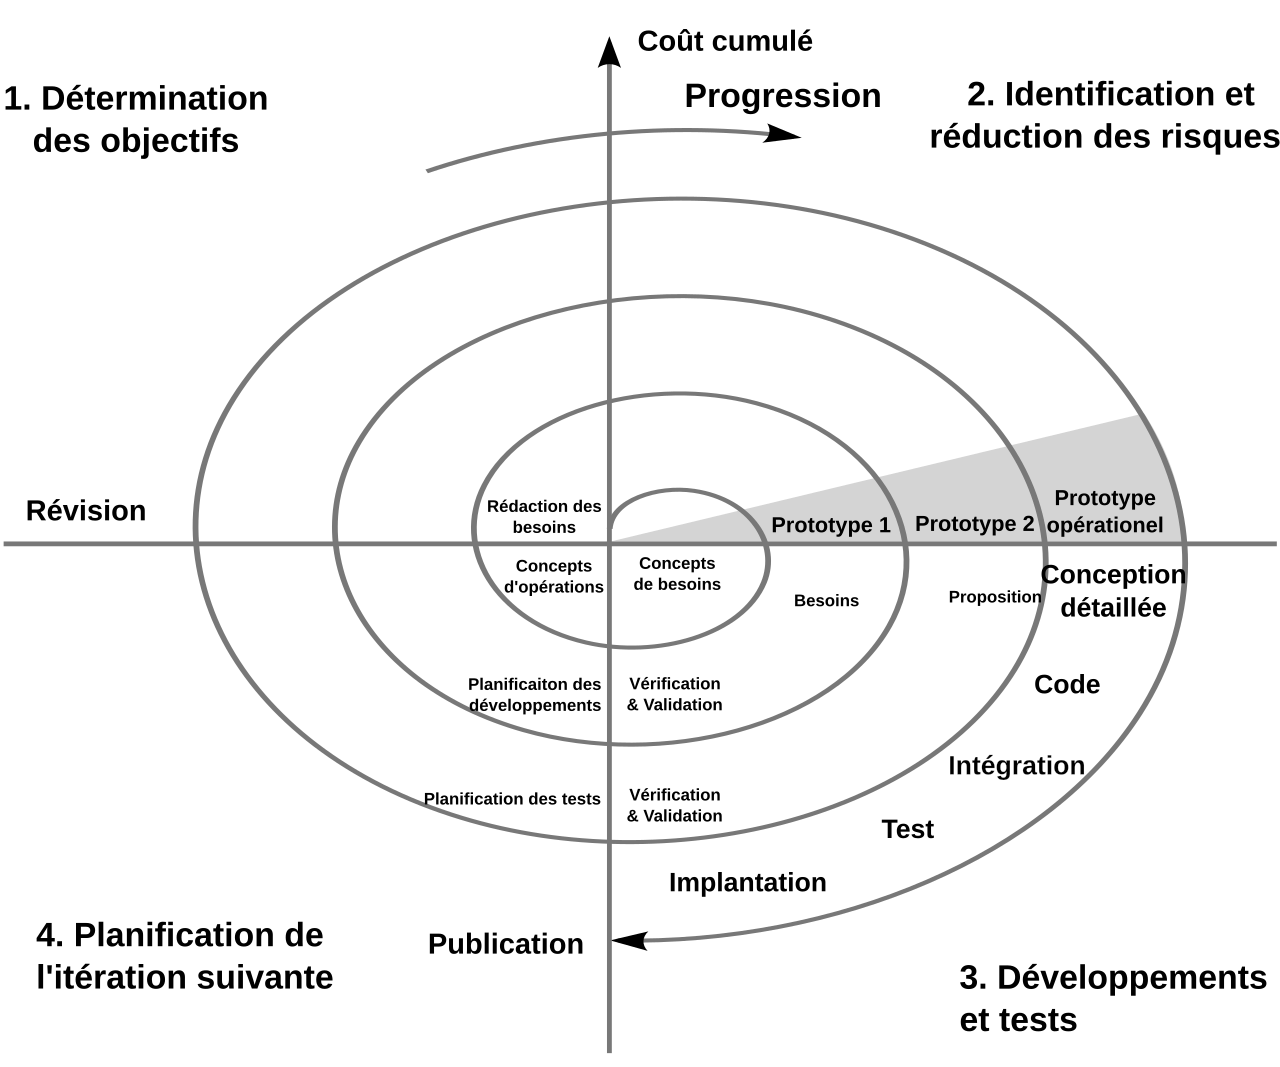
\includegraphics[width=0.92\textwidth]{public/ch2-modele-spirale.png}
			\caption{Modèle en spirale — enchaînement des six cycles de développement KODA}
			\label{fig:ch1-modele-spirale}
		\end{figure}
	}{}
	
	\vspace{0.3cm}
	\noindent\textbf{Artefacts et traçabilité}\\
	À chaque tour, des livrables assurent la continuité entre les cycles~:
	\begin{itemize}
		\item \textbf{Besoins et périmètre} mis à jour (utilisateur, sécurité, mémoire).
		\item \textbf{Architecture et intégration} (schémas, interfaces entre robot,
		logiciel de réflexion, application).
		\item \textbf{Réalisation et recette} du cycle en cours (tests, démonstration,
		correctifs avant le tour suivant).
	\end{itemize}
	
	\section{Conclusion}
	
	
Ce chapitre a établi le contexte du projet KODA. En identifiant les lacunes critiques des assistants virtuels actuels — notamment le manque de personnalité, de réflexion autonome et d'intégration embarquée — nous avons défini notre solution innovante. Le \textbf{modèle en spirale} et les six cycles de développement posent une feuille de route incrémentale, adaptée à la complexité d'un système distribué entre compagnon physique, réflexion et pilotage mobile.

Le chapitre suivant, \textbf{«\,Préparation du Projet\,»}, formalise les besoins, la méthodologie de développement \textbf{en spirale} par cycles successifs et les environnements techniques retenus pour mener à bien la réalisation de KODA.
	
	
	%================================================================
	%  CHAPITRE II : Préparation du Projet
	%================================================================
	\chapter{Préparation du Projet}
	\chaptermark{Préparation du Projet}
	
	\section{Introduction du chapitre}
	
	Ce chapitre pose les fondations ingénierie du projet \textbf{KODA} avant d'entrer dans
	le détail technique des cycles de réalisation. Nous y traduisons l'intention du
	chapitre~I en \textbf{exigences traçables} (fonctionnelles et non fonctionnelles),
	en \textbf{vision architecturale} et en \textbf{périmètre d'acteurs}. Nous y
	présentons également la \textbf{méthodologie de pilotage} retenue : le \textbf{modèle
	en spirale}, fondé sur des \textbf{cycles de développement successifs} —
	et non sur une succession de sprints Scrum — où chaque tour de spirale livre un
	incrément (couche ou sous-système) intégrable et réévalue les risques avant le tour
	suivant. Enfin, nous documentons les environnements matériel et logiciel qui ont
	encadré la production du prototype.
	
	%----------------------------------------------------------------
	\section{Spécification des besoins}
	%----------------------------------------------------------------
	
	\subsection{Spécifications des besoins fonctionnels}
	
	Les besoins fonctionnels précisent \textit{ce que} KODA doit offrir à l'utilisateur,
	sans décrire encore les choix d'implémentation. Ils reprennent la problématique du
	chapitre~I~: un \textbf{compagnon de vie} capable de présence, de réflexion et
	d'accompagnement personnalisé, et non un simple exécuteur de commandes.
	
	\begin{itemize}
		\item \textbf{Dialoguer naturellement :} l'utilisateur s'adresse à KODA à l'oral ou
		par message ; le compagnon comprend la demande, y répond de façon claire et
		pertinente, et adapte son ton à la situation (explication, conseil, réconfort).
		Lorsque la question appelle une réponse immédiate (arrêt, mot de passe, musique,
		déplacement), KODA réagit sans détour ; sinon, il prend le temps d'analyser avant
		de répondre.
		\item \textbf{Se souvenir et personnaliser :} KODA reconnaît les personnes avec
		lesquelles il interagit, retient leurs présentations, leurs préférences et les
		éléments importants de leurs échanges (notes, informations personnelles). Il peut
		répondre en s'appuyant sur ce qu'il sait déjà de l'utilisateur, ou traiter une
		question générale sans tout reconsulter ; la mémoire est consolidée au fil du
		temps pour garder une continuité dans la relation.
		\item \textbf{Reconnaître et accueillir :} le compagnon identifie l'interlocuteur
		(visage, contexte) et adapte son comportement~: accueil personnalisé pour une
		personne connue, invitation à se présenter pour un visiteur inconnu, conformément
		à l'objectif de présence humaine évoqué au chapitre~I.
		\item \textbf{Être présent physiquement :} le robot matérialise l'interaction
		(captures, parole, déplacements ou signaux prévus par le prototype) et reste
		relié au reste du système pour que l'expérience ne se limite pas à un écran ou à
		une enceinte déconnectée du corps du compagnon.
		\item \textbf{Permettre le pilotage à distance :} via l'application mobile,
		l'utilisateur configure la personnalité de KODA (nom, caractère, langue, etc.),
		suit son activité et supervise son compagnon au quotidien, comme annoncé dans la
		solution proposée au chapitre~I.
		\item \textbf{Protéger l'usage et l'environnement :} KODA fonctionne selon des
		modes ouvert ou protégé (mot de passe), afin de limiter l'accès aux fonctions
		sensibles lorsque le compagnon est en mode sécurisé~; cette exigence répond au
		besoin, formulé au chapitre~I, d'allier accompagnement humain et gestion
		responsable de l'environnement domestique.
	\end{itemize}
	
	\IfFileExists{public/ch2-besoins-fonctionnels.png}{%
		\begin{figure}[htbp]
			\centering
			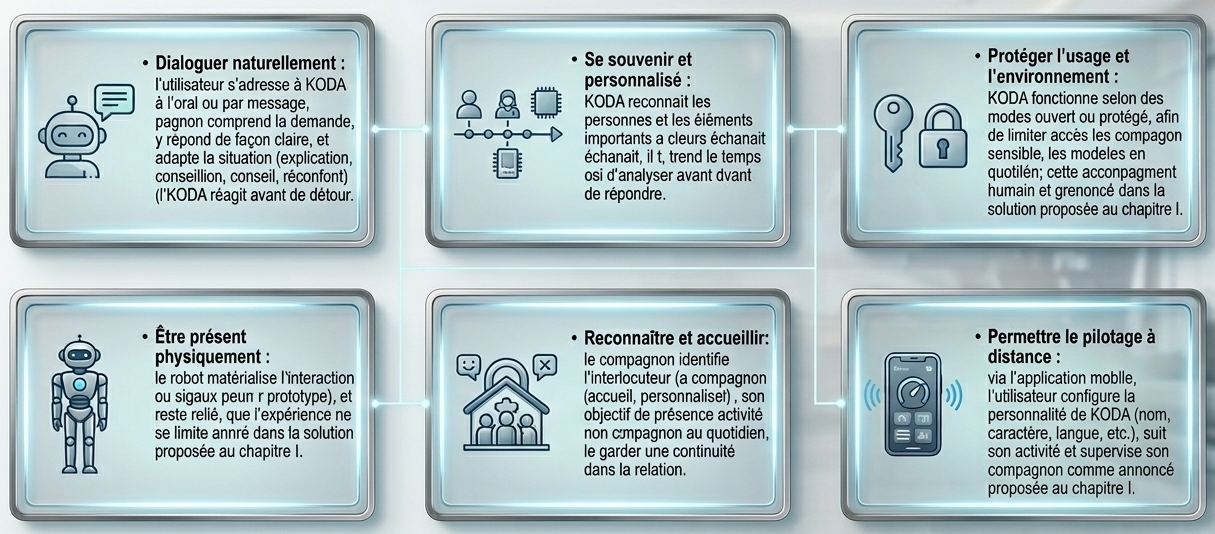
\includegraphics[width=0.95\textwidth]{public/ch2-besoins-fonctionnels.png}
			\caption{Synthèse visuelle des besoins fonctionnels KODA (chapitre~II)}
			\label{fig:ch2-besoins-f}
		\end{figure}
	}{%
		\begin{center}
			\fbox{\begin{minipage}{0.88\textwidth}\centering\vspace{1.2em}
				\textit{Figure optionnelle — générer \texttt{public/ch2-besoins-fonctionnels.png}\\
				(voir \texttt{prompts/ch2-images-generation-prompts.txt}).}
				\vspace{1.2em}\end{minipage}}
		\end{center}
	}
	
	\subsection{Spécification des besoins non fonctionnels}
	
	Les besoins non fonctionnels décrivent \textit{comment} le système doit se comporter
	pour être acceptable au quotidien~: fiabilité, confiance, simplicité d'évolution.
	Ils complètent les besoins fonctionnels sans entrer dans le détail des outils retenus
	aux chapitres techniques suivants.
	
	\begin{itemize}
		\item \textbf{Réactivité perçue :} les réponses du compagnon doivent paraître
		fluides à l'utilisateur, y compris lorsque le traitement s'appuie sur des
		services en ligne (recherche, synthèse vocale, etc.)~; les échanges déjà connus ne
		doivent pas systématiquement être retraités comme s'il n'y avait aucune mémoire.
		\item \textbf{Continuité de service :} une coupure partielle d'un service distant
		ne doit pas faire perdre l'essentiel des données ni bloquer durablement
		l'interaction~; les informations importantes (profils, historiques, paramètres)
		restent conservées de façon durable.
		\item \textbf{Confiance et respect de la vie privée :} seules les personnes
		autorisées accèdent aux fonctions sensibles~; les identifiants et données
		personnelles sont protégés, et le compagnon n'expose pas inutilement ce qu'il
		sait de l'utilisateur.
		\item \textbf{Clarté pour l'équipe projet :} la logique est organisée par blocs
		(dialogue, mémoire, robot, application) afin de pouvoir corriger ou enrichir une
		partie sans remettre en cause tout le système~; les scénarios principaux restent
		documentés pour la validation en fin de cycle.
		\item \textbf{Ouverture aux évolutions :} il doit être possible d'ajouter une
		nouvelle capacité (type de question, écran mobile, capteur) en s'appuyant sur
		l'architecture globale du chapitre~I, sans repartir d'une conception entièrement
		nouvelle.
		\item \textbf{Accessibilité d'usage :} l'application de pilotage et les modes du
		compagnon restent compréhensibles pour un utilisateur non spécialiste, en ligne
		avec l'objectif d'un compagnon \og accessible \fg{} par rapport aux robots
		professionnels coûteux évoqués dans l'analyse de l'existant.
	\end{itemize}
	
	\subsection{Architecture du système}
	
	L'architecture cible est \textbf{multicouche} et \textbf{distribuée} : un moteur
	d'automatisation (\textbf{n8n}) concentre la logique métier conversationnelle ; un
	\textbf{backend Python (FastAPI)} centralise les accès données et les intégrations
	cloud ; un \textbf{noyau embarqué (Raspberry Pi)} assure le lien avec le monde
	physique ; une \textbf{application mobile} prolonge l'expérience utilisateur ; une
	\textbf{base PostgreSQL} matérialise la mémoire long terme. La
	figure~\ref{fig:ch2-architecture-systeme} (chapitre~I et~II) illustre cette décomposition ; les cycles
	de développement du présent rapport s'alignent sur ces blocs pour réduire le
	rayon d'intégration à chaque itération.
	
	\begin{figure}[htbp]
		\centering
		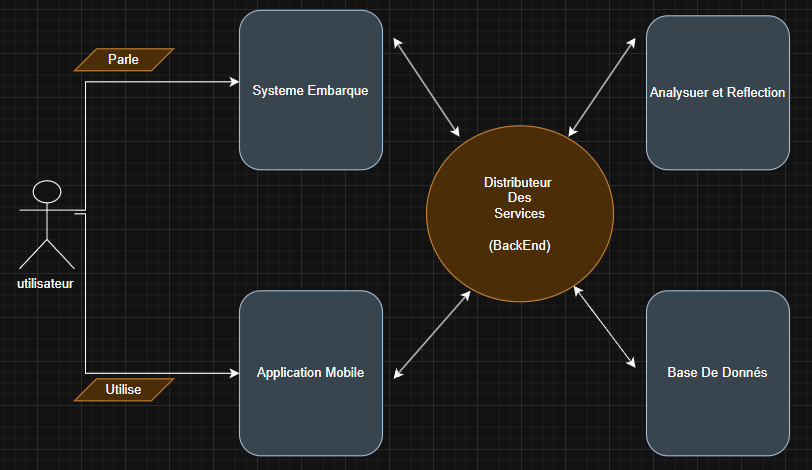
\includegraphics[width=0.95\textwidth]{public/ch2-architecture-systeme.png}
		\caption{Architecture multicouche du système KODA (vue chapitre~II)}
		\label{fig:ch2-architecture-systeme}
	\end{figure}
	
	\subsection{Identification des acteurs}
	
	On distingue notamment :
	\begin{itemize}
		\item l'\textbf{Utilisateur final} (personne qui dialogue avec KODA et configure
		l'application) ;
		\item le \textbf{système KODA} (ensemble logiciel/matériel) ;
		\item le \textbf{Distributeur de services} (backend) en tant qu'intermédiaire
		technique ;
		\item les \textbf{services externes} (Supabase, OpenRouter pour les LLM,
		SerpAPI pour la recherche musique au Block~1, Azure pour la voix et la vision) ;
		\item l'\textbf{organisme d'accueil} et l'\textbf{équipe projet} (rôles de pilotage
		et de validation).
	\end{itemize}
	
	% Figure acteurs : page portrait dediee, rotation 90° pour lisibilite
	\IfFileExists{public/ch2-diagramme-acteurs.png}{%
		\clearpage
		\begin{figure}[p]
			\centering
			\vfill
			\rotatebox{-90}{%
				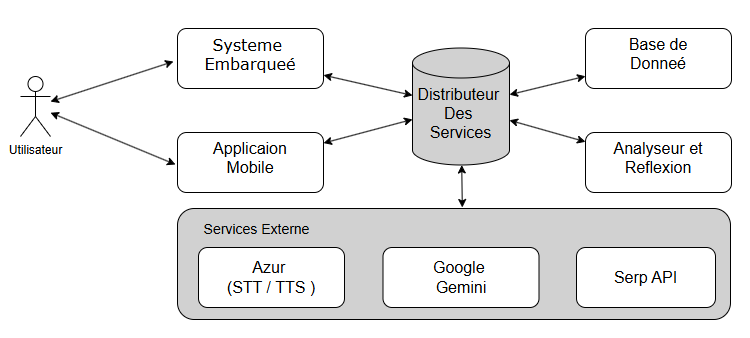
\includegraphics[
					width=0.92\textheight,
					keepaspectratio
				]{public/ch2-diagramme-acteurs.png}%
			}%
			\vspace{1.2em}
			\caption{Acteurs principaux et contexte d'intégration du système KODA}
			\label{fig:ch2-acteurs}
			\vfill
		\end{figure}
		\clearpage
	}{%
		\begin{center}
			\fbox{\begin{minipage}{0.88\textwidth}\centering\vspace{1.2em}
				\textit{Diagramme des acteurs — exporter PlantUML vers \texttt{public/ch2-diagramme-acteurs.png}\\
				(fichier source : \texttt{plantuml/ch2-diagramme-acteurs.puml}).}
				\vspace{1.2em}\end{minipage}}
		\end{center}
	}
	
	%----------------------------------------------------------------
	\section{Pilotage du projet — Modèle en spirale et cycles de développement}
	%----------------------------------------------------------------
	
	Contrairement à une approche \textbf{Agile Scrum} fondée sur des \textit{sprints}
	de durée fixe avec cérémonies prescrites (daily, review, rétrospective), nous avons
	retenu le \textbf{modèle en spirale} : à chaque itération, une portion du produit
	(cycle thématique : workflows n8n, backend, matériel, logiciel embarqué, mobile,
	validation) est \textbf{spécifiée}, \textbf{réalisée} puis \textbf{intégrée} au
	système global, avec une \textbf{réévaluation des risques} et des priorités avant le
	tour suivant. Chaque cycle produit un incrément \textbf{testable} et raccordé aux
	livrables des tours précédents, jusqu'à stabiliser l'écosystème KODA complet.
	
	\subsection{Équipe et rôles}
	
	Le projet est conduit par une \textbf{équipe de projet de fin d'études} (DSI3.2,
	ISET Mahdia), en binôme, sous la responsabilité d'un \textbf{encadrant académique}
	et en lien avec l'\textbf{organisme d'accueil} MicroEdition (cf. chapitre~I). Les
	rôles se répartissent entre conception des workflows n8n, développement backend,
	intégration embarquée, développement mobile et campagne de tests, avec des points
	de synchronisation à la fin de chaque cycle pour valider l'intégration incrémentale.
	
	\subsection{Découpage du travail : six cycles}
	
	Le périmètre fonctionnel est découpé en six cycles \textbf{ordonnés logiquement} —
	sans équivalence directe avec des sprints Scrum — comme suit :
	
	\begin{enumerate}
		\item \textbf{Cycle~1 — Workflow et n8n :} conception des webhooks, blocs de
		traitement (classification d'intention, analyseur de dépendance mémoire,
		consolidation, proactivité), intégration des API LLM et recherche.
		\item \textbf{Cycle~2 — Backend :} Distributeur de services (FastAPI), accès
		PostgreSQL / Supabase, Clean Architecture, endpoints pour le robot et le mobile.
		\item \textbf{Cycle~3 — Système embarqué, partie matérielle :} choix et câblage
		des capteurs, actionneurs, alimentation, mécanique ou support physique associé au
		Raspberry Pi selon le prototype.
		\item \textbf{Cycle~4 — Système embarqué, partie logicielle (Raspberry Pi) :}
		logiciel embarqué, communication avec le backend, gestion des flux audio/vidéo
		locaux, robustesse sur carte ARM.
		\item \textbf{Cycle~5 — Cross-plateforme :} application mobile (configuration,
		suivi, notifications), parcours utilisateur unifiés Android/iOS.
		\item \textbf{Cycle~6 — Tests et validation :} tests unitaires et d'intégration,
		scénarios bout-en-bout, validation des besoins non fonctionnels (sécurité,
		performance).
	\end{enumerate}
	
	\begin{table}[htbp]
		\centering
		\caption{Vue synthétique des cycles et livrables attendus}
		\label{tab:cycles_koda}
		\renewcommand{\arraystretch}{1.25}
		\begin{tabular}{|c|p{4.2cm}|p{7.5cm}|}
			\hline
			\textbf{Cycle} & \textbf{Thème} & \textbf{Livrable principal} \\
			\hline
			1 & Workflow n8n & Webhooks opérationnels, prompts et routages stabilisés \\
			\hline
			2 & Backend & API documentée, persistance, intégrations cloud \\
			\hline
			3 & Embarqué HW & Plateforme physique prête à accueillir le logiciel \\
			\hline
			4 & Embarqué SW (Pi) & Services locaux et dialogue avec le Distributeur \\
			\hline
			5 & Cross-plateforme & Application mobile utilisable sur les cibles \\
			\hline
			6 & Tests \& validation & Rapport de recette, correctifs de fin de projet \\
			\hline
		\end{tabular}
	\end{table}
	
	\begin{figure}[htbp]
		\centering
		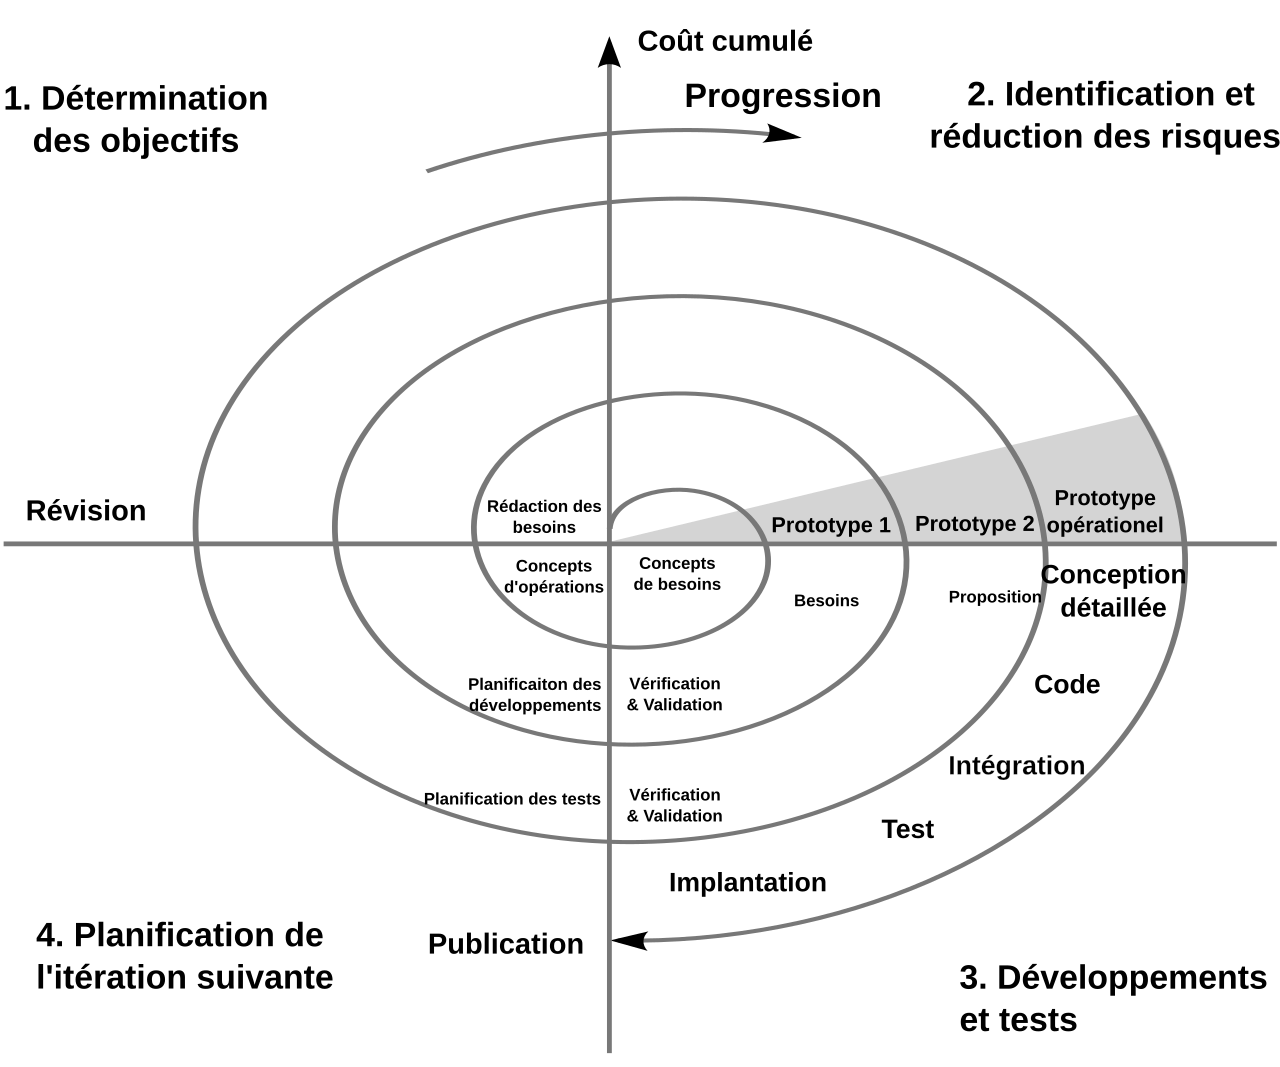
\includegraphics[width=0.95\textwidth]{public/ch2-modele-spirale.png}
		\caption{Modèle en spirale et enchaînement des six cycles de développement KODA}
		\label{fig:ch2-modele-spirale}
	\end{figure}
	
	%----------------------------------------------------------------
	\section{Planification des cycles}
	%----------------------------------------------------------------
	
	La planification ne s'exprime pas en \textbf{sprints} de deux semaines mais en
	\textbf{jalons de cycles} : chaque cycle se termine par une \textbf{démonstration
	intégrée} (workflow branché sur le backend, backend branché sur la base, puis
	ajout du Raspberry Pi, etc.). Les dépendances imposent un ordre raisonnable : le
	moteur n8n (cycle~1) et le backend (cycle~2) peuvent avancer en parallèle partiel,
	mais la validation bout-en-bout (cycle~6) recouvre l'ensemble. Le calendrier
	académique du PFE (nombre de semaines, séances de suivi, livrables intermédiaires)
	structure la cadence réelle ; le \textbf{modèle en spirale} en garantit la
	\textbf{cohérence} : aucun cycle ne clôt sans critères d'acceptation liés aux
	chapitres techniques correspondants du rapport.
	
	\IfFileExists{public/ch2-planification-cycles.png}{%
		\begin{figure}[htbp]
			\centering
			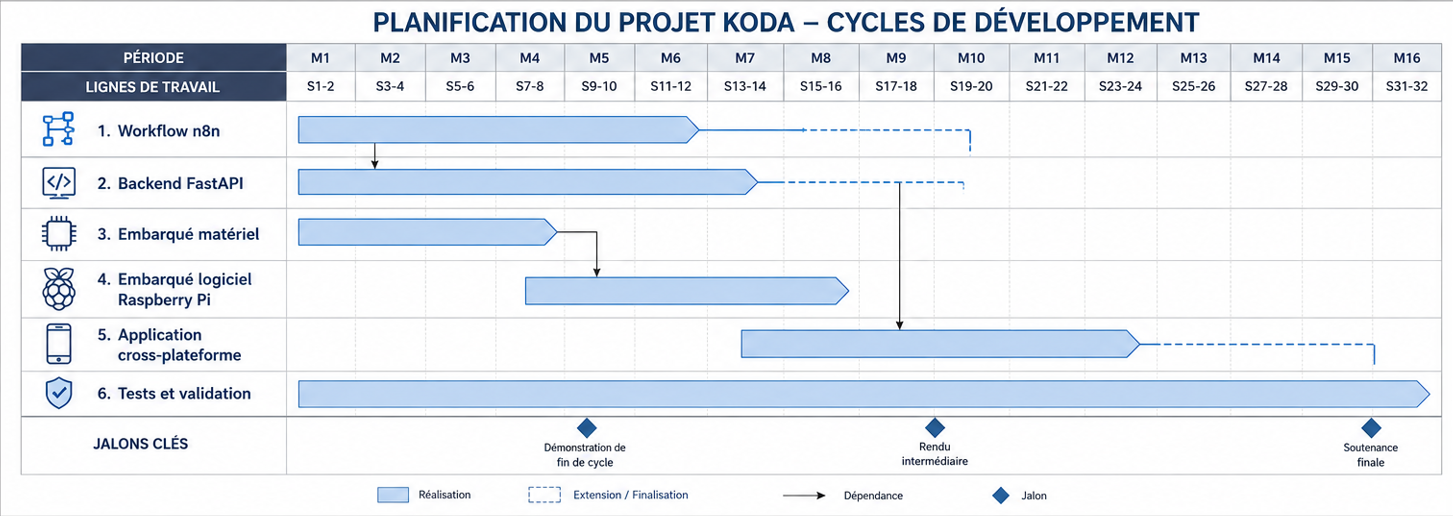
\includegraphics[width=\textwidth]{public/ch2-planification-cycles.png}
			\caption{Planification des cycles : jalons, chevauchements et dépendances}
			\label{fig:ch2-planification-cycles}
		\end{figure}
	}{%
		\begin{center}
			\fbox{\begin{minipage}{0.88\textwidth}\centering\vspace{1.2em}
				\textit{Figure à ajouter — \texttt{public/ch2-planification-cycles.png}\\
				(prompt : voir \texttt{prompts/ch2-images-generation-prompts.txt}).}
				\vspace{1.2em}\end{minipage}}
		\end{center}
	}
	
	%----------------------------------------------------------------
	\section{Architecture}
	%----------------------------------------------------------------
	
	\subsection{Architecture de l'application}
	
	Au-delà du schéma global (chapitre~I), l'architecture applicative distingue :
	\textbf{(a)} la couche \textit{présentation} (mobile) ; \textbf{(b)} la couche
	\textit{orchestration intelligente} (n8n) ; \textbf{(c)} la couche
	\textit{services} (FastAPI) ; \textbf{(d)} la couche \textit{données} (PostgreSQL) ;
	\textbf{(e)} la couche \textit{embarquée} (Raspberry Pi). Les communications
	principales suivent le modèle requête-réponse REST et événements asynchrones selon
	les besoins (temps réel, webhooks). Cette structuration facilite le parallélisme
	des cycles tout en conservant des interfaces stables entre équipes.
	
	\subsubsection{Architecture en oignon (\textit{Onion Architecture}) du backend}
	
	Le \textbf{Distributeur de services} (backend Python, cycle~2) adopte une
	\textbf{architecture en oignon} : les couches sont organisées en \textbf{anneaux
	concentriques}, du plus stable au plus volatile. Au \textbf{c\oe{}ur} se trouvent le
	\textbf{domaine métier} (entités, règles) ; autour, les \textbf{cas d'usage}
	orchestrent les scénarios sans dépendre des frameworks ; puis viennent les
	\textbf{adaptateurs} (API REST, sérialisation, accès données) ; en périphérie, la
	\textbf{infrastructure} (FastAPI, Supabase, SDK Azure, clients HTTP vers n8n ou le
	robot). Les dépendances pointent \textbf{toujours vers l'intérieur}, ce qui isole
	la logique métier des technologies et facilite les tests unitaires sur le domaine.
	
	Ce modèle — popularisé notamment par Jeffrey Palermo sous le nom d'\textit{Onion
	Architecture} — recoupe les principes de la \textbf{Clean Architecture} détaillés
	au chapitre du cycle~2 : les deux visions décrivent des couches concentriques et la
	règle d'inversion des dépendances ; l'«\,oignon\,» met l'accent sur la \textbf{testabilité}
	du noyau et sur le fait que l'infrastructure soit interchangeable sans toucher au
	c\oe{}ur du système. Ainsi, le backend KODA reste cohérent avec la vision multicouche
	de la figure~\ref{fig:ch2-architecture-systeme} tout en précisant sa structure interne.
	
	%----------------------------------------------------------------
	\section{Environnement de Developement}
	%----------------------------------------------------------------
	
	\subsection{Environnement matériel}
	
	Le développement s'appuie sur des postes de travail type PC (processeur multi-c\oe{}urs,
	au moins 8~Go de RAM recommandés pour les outils de conteneurisation et les IDE),
	un \textbf{Raspberry Pi} cible pour les tests embarqués, périphériques audio/vidéo
	selon les besoins du robot, et un smartphone ou émulateur pour la couche mobile.
	Un accès Internet stable est nécessaire pour Supabase, OpenRouter, SerpAPI et
	Azure durant l'intégration.
	
	\IfFileExists{public/ch2-environnement-materiel.png}{%
		\begin{figure}[htbp]
			\centering
			\includegraphics[width=0.92\textwidth]{public/ch2-environnement-materiel.png}
			\caption{Environnement matériel de développement et de test (poste, Raspberry Pi, robot)}
			\label{fig:ch2-env-materiel}
		\end{figure}
	}{%
		\begin{center}
			\fbox{\begin{minipage}{0.88\textwidth}\centering\vspace{2em}
				\textit{Emplacement réservé — photographie à insérer sous le nom\\
				\texttt{public/ch2-environnement-materiel.png} (PC, Raspberry Pi, périphériques du robot).}
				\vspace{2em}\end{minipage}}
		\end{center}
	}
	
	%----------------------------------------------------------------
	\section{Environnement logiciel}
	%----------------------------------------------------------------
	
	\subsection{Outils de développement et modélisation}
	
	\begin{itemize}
		\item \textbf{n8n} (self-hosted ou cloud) pour l'édition des workflows ;
		\item \textbf{Visual Studio Code} ou équivalent pour Python, Dart et LaTeX ;
		\item \textbf{Git} pour le versioning ;
		\item \textbf{PlantUML} / captures d'écran pour les diagrammes de séquence et de
		cas d'utilisation ;
		\item \textbf{Supabase Studio} pour l'administration PostgreSQL ;
		\item \textbf{Docker} (le cas échéant) pour le déploiement du backend et la
		reproductibilité des environnements.
	\end{itemize}
	
	\subsection{Langages et frameworks utilisés}
	
	\begin{itemize}
		\item \textbf{JavaScript} (expressions n8n, nœuds Code) ;
		\item \textbf{Python~3} avec \textbf{FastAPI}, SQLAlchemy, asyncpg, SDK Azure et
		intégrations Gemini/OpenRouter côté Distributeur ;
		\item \textbf{SQL} (PostgreSQL) ;
		\item \textbf{Dart / Flutter} pour l'application cross-plateforme ;
		\item \textbf{Bash} et utilitaires système sur Raspberry Pi OS.
	\end{itemize}
	
	\begin{figure}[htbp]
		\centering
		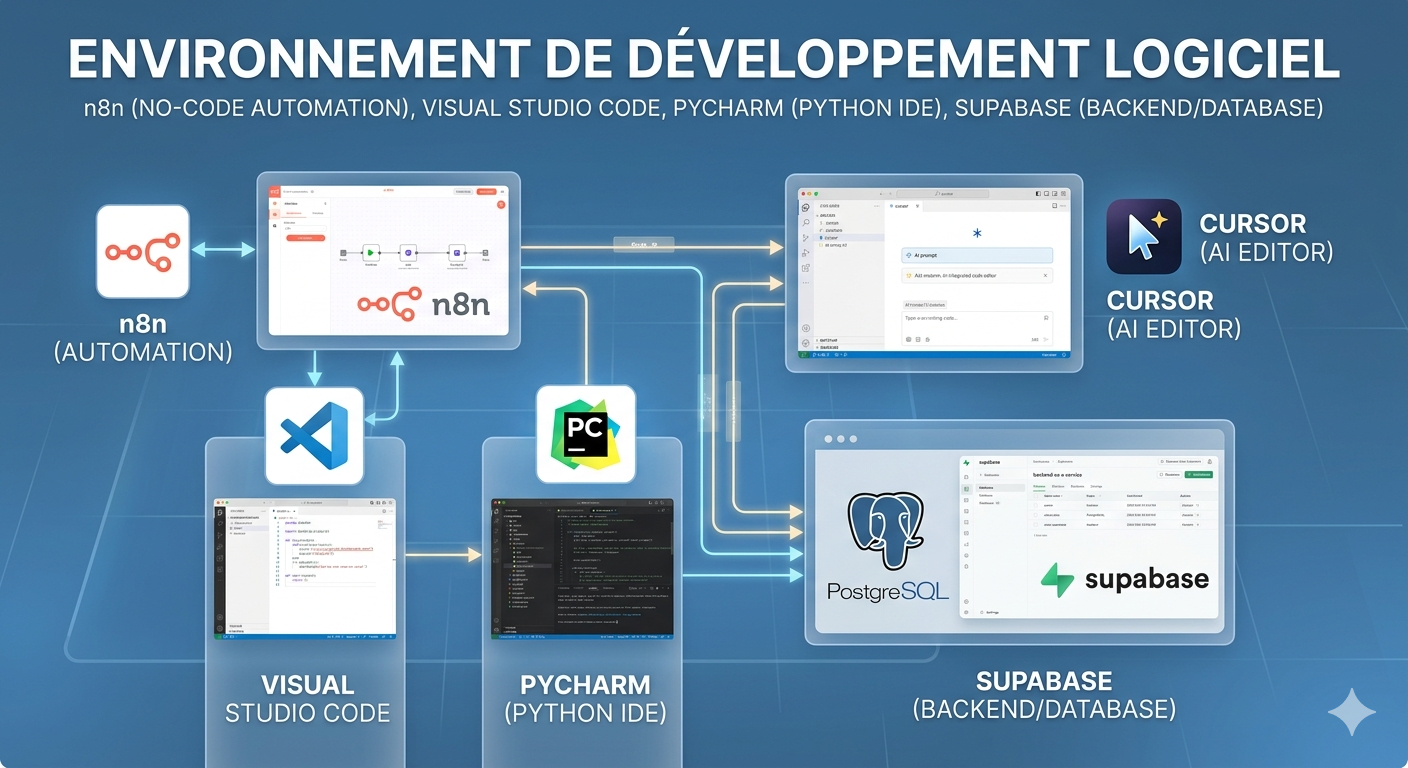
\includegraphics[width=0.95\textwidth]{public/ch2-environnement-logiciel.png}
		\caption{Environnement logiciel : outils de développement et chaîne technique (chapitre~II)}
		\label{fig:ch2-env-logiciel}
	\end{figure}
	
	%----------------------------------------------------------------
	\section{Figures et diagrammes prévus pour ce chapitre}
	%----------------------------------------------------------------
	
	Pour illustrer le chapitre~II dans le PDF final, les captures et exports suivants
	 sont recommandés. Les noms de fichiers sont normalisés \textbf{sans espace}
	(dossier \texttt{public/}) afin d'éviter les erreurs de compilation \LaTeX{} ; il
	suffit de créer chaque fichier sous ce nom puis d'insérer
	\texttt{\textbackslash includegraphics} dans la section concernée.
	

	
	\noindent\textbf{Réutilisation possible :} la figure d'architecture multicouche du
	chapitre~I (\texttt{public/ch2-architecture-systeme.png}) peut être réutilisée ou
	déclinée pour d'autres sections après recadrage ou légende adaptée au
	§\,2.2.3 / 2.5. Le \textbf{modèle en spirale} introduit au chapitre~I est détaillé
	ici (cycles, planification, figure~\ref{fig:ch2-modele-spirale}).
	
	%----------------------------------------------------------------
	\section{Conclusion}
	%----------------------------------------------------------------
	
	Ce chapitre a cadré la préparation de KODA : besoins fonctionnels et non
	fonctionnels, acteurs, architecture de référence, environnements, et surtout un
	\textbf{modèle en spirale} articulé en six cycles — en rupture avec une
	gestion purement Scrum/sprint, tout en conservant l'esprit d'incrémentalité et de
	revue de fin de cycle. Le chapitre suivant détaille le \textbf{Cycle~1} (\textbf{Analyseur et réflexion})~: workflows n8n.
	
	%================================================================
	%  CHAPITRE III : Analyseur et réflexion
	%================================================================
	\chapter{Cycle 1 : ANALYSEUR ET RÉFLEXION}
	\chaptermark{Cycle 1 --- Analyseur et réflexion}
	
	% Couleur principale pour les blocs internes
	\definecolor{kodablue}{RGB}{0, 84, 166}
	\definecolor{kodasection}{RGB}{30, 120, 200}
	\definecolor{kodablock}{RGB}{20, 100, 180}
	
	\section{Introduction}
	
	Le \textbf{Cycle~1 --- Analyseur et réflexion} constitue le \textbf{moteur cognitif} de KODA.
	Son rôle est double~: assurer la \textbf{génération des réponses} lorsque l'utilisateur
	pose une question, et alimenter la \textbf{spontanéité} du robot lorsqu'il prend
	l'initiative de parler. L'objectif poursuivi est de développer un système capable
	d'\textbf{accueillir une question}, de la \textbf{comprendre dans son contexte},
	d'effectuer les \textbf{recherches et consultations} nécessaires (mémoire, profil,
	services externes), puis de \textbf{formuler et restituer une réponse} adaptée.
	
	La chaîne de traitement --- de l'entrée utilisateur à la réponse --- forme une
	\textbf{ligne de processus} successifs. Les \textbf{outils d'automatisation de flux}
	offrent une meilleure lisibilité et un débogage par étape que du code monolithique~;
	la \textbf{bonne pratique} retenue est la plateforme \textbf{n8n}, auto-hébergée et
	adaptée aux pipelines mêlant règles métier et intelligence artificielle.
	
	Trois \textbf{webhooks} n8n structurent ce cycle. Après les fondements théoriques, la
	modélisation globale puis l'analyse détaillée de chaque flux, le lecteur dispose d'une
	vue complète du moteur d'analyse et de réflexion.
	
	%----------------------------------------------------------------
	\section{Fondements Théoriques}
	%----------------------------------------------------------------
	
	Cette section pose le \textbf{cadre cognitif} du Cycle~1. Elle explique, en termes
	généraux, comment une personne comprend une question et choisit une réponse~; elle ne
	décrit pas encore les outils informatiques (n8n, webhooks, base de données), traités
	aux sections suivantes.
	
	\subsection{Que signifie «~théorie du double traitement~»~?}
	
	L'expression \textbf{théorie du double traitement} (\textit{dual-process theory}) désigne
	une idée simple~: face à une question, l'esprit humain ne suit pas toujours le même
	chemin. Selon la situation, il peut répondre \textbf{presque tout de suite} en s'appuyant
	sur ce qu'il sait déjà, ou réfléchir \textbf{plus longtemps} en recomposant des
	éléments mémorisés. Ce modèle, largement diffusé par Daniel Kahneman
	(\textit{Thinking, Fast and Slow}, 2011), aide à comprendre pourquoi certaines réponses
	sont instantanées et d'autres demandent un effort conscient.
	
	En psychologie cognitive, on parle souvent de \textbf{cognition intuitive} (rapide) et de
	\textbf{cognition analytique} (lente), plutôt que de «~système~1~» et «~système~2~»~:
	ces derniers termes sont des étiquettes de laboratoire peu parlantes pour le lecteur
	non spécialiste. Nous les remplaçons donc par des formulations explicites ci-dessous.
	
	\subsection{Réflexion rapide et réflexion lente}
	
	\subsubsection{Réflexion rapide~: réutiliser la mémoire déjà présente}
	
	La \textbf{réflexion rapide} correspond à une \textbf{cognition heuristique}~: le cerveau
	repère un schéma connu et active presque aussitôt un souvenir, une habitude ou une
	règle déjà apprise. La réponse paraît «~évidente~» parce qu'elle ne reconstruit pas
	toute la situation depuis zéro~; elle \textbf{s'appuie sur la mémoire déjà là}~:
	souvenirs récents de la conversation, image de l'interlocuteur, faits appris par cœur,
	gestes routiniers (saluer, donner son prénom, réciter une capitale connue).
	
	Cette voie est \textbf{économique en attention}~: elle convient lorsque la question
	ressemble à quelque chose de déjà vécu ou lorsque l'information demandée est
	directement stockée. Elle peut toutefois se tromper si le contexte a changé sans que
	l'on s'en aperçoive (réponse trop hâtive fondée sur une analogie fausse).
	
	\subsubsection{Réflexion lente~: analyser la mémoire pour fabriquer une réponse}
	
	La \textbf{réflexion lente} correspond à une \textbf{cognition analytique}~: le cerveau
	\textbf{parcourt}, \textbf{compare} et \textbf{combine} des éléments en mémoire pour
	\textbf{construire} une réponse nouvelle. Elle intervient lorsque la question est
	floue, inédite, émotionnellement chargée ou exige de croiser plusieurs souvenirs
	(passés lointains, préférences de l'interlocuteur, règles implicites de politesse,
	conséquences d'un choix).
	
	Elle est \textbf{plus lente} précisément parce qu'elle ne se contente pas d'un rappel
	automatique~: elle \textbf{analyse} le contenu mémorisé (épisodes, connaissances,
	sentiments) avant de formuler une phrase adaptée. On peut encore corriger ou affiner
	la réponse une fois qu'elle est énoncée (reformulation, nuance, excuse).
	
	Les deux voies \textbf{coopèrent}~: la réflexion rapide propose souvent une première
	piste~; la réflexion lente peut la confirmer, la nuancer ou la remplacer.
	
	\subsection{Comment une question est comprise avant la réponse}
	
	Qu'une question arrive à l'\textbf{oral} ou à l'\textbf{écrit}, le déroulement
	général est le suivant~:
	\begin{enumerate}[leftmargin=*, itemsep=0.25em]
		\item \textbf{Percevoir la question}~: entendre ou lire les mots, filtrer le bruit,
		porter attention à l'interlocuteur.
		\item \textbf{Comprendre le sens}~: saisir ce qui est demandé (information, avis,
		souhait, plaisanterie) et le contexte immédiat (qui parle, de quoi on parlait
		juste avant).
		\item \textbf{Mobiliser la mémoire}~: faire remonter des souvenirs utiles~:
		échanges récents, connaissances générales, image de la relation avec cette personne.
		\item \textbf{Choisir la voie rapide ou lente}~: si un souvenir pertinent «~saute aux
		yeux~», la réflexion rapide suffit~; sinon, la réflexion lente assemble et vérifie
		les éléments avant de répondre.
		\item \textbf{Formuler et, si besoin, ajuster}~: prononcer ou écrire la réponse, puis
		la corriger si elle sonne faux ou incomplet.
	\end{enumerate}
	
	\IfFileExists{public/ch3-double-traitement-humain.png}{%
		\kodafigureL[0.9\textwidth]{public/ch3-double-traitement-humain.png}{De la question à la réponse~: réflexion rapide (mémoire déjà présente) ou réflexion lente (analyse puis construction)}{fig:ch3-double-traitement-humain}
	}{}
	
	\subsection{Intérêt pour un compagnon conversationnel comme KODA}
	
	Un robot compagnon doit imiter cette logique humaine~: parfois répondre vite en
	réutilisant ce qui vient d'être dit ou mémorisé sur l'utilisateur~; parfois prendre
	le temps d'\textbf{interpréter} la demande et d'\textbf{élaborer} une réponse plus
	personnalisée. Le Cycle~1 matérialise ce principe dans l'implémentation technique,
	décrite à partir de la section~\ref{sec:modelisation-cycle1}~; la figure~\ref{fig:archic}
	en donne une vue d'ensemble une fois les notions d'outillage posées.
	
	\noindent\underline{\textbf{Références :} Kahneman, D. (2011). \textit{Thinking, Fast and Slow}~;
	Evans, J.St.B.T. (2008). Dual-processing accounts of reasoning, judgment, and social cognition.}
	\FloatBarrier
	
	%----------------------------------------------------------------
	\section{Définitions Fondamentales}
	%----------------------------------------------------------------
	
	Le Cycle~1 s'appuie sur \textbf{n8n} (automatisation par workflows et nœuds, données
	JSON, auto-hébergement) et sur trois \textbf{webhooks} HTTP déclenchant les pipelines
	d'analyse, de synthèse et de spontanéité. Les appels aux modèles de langage passent
	par \textbf{OpenRouter}, agrégateur d'API modèles utilisé dans les nœuds n8n de type
	\textit{Basic LLM Chain} ou \textit{AI Agent}.
	
	\subsection{Grand modèle de langage (LLM)}
	
	Un \textbf{grand modèle de langage} — en anglais \textit{Large Language Model}, souvent
	abrégé \textbf{LLM} — est un modèle de \textbf{apprentissage profond} entraîné sur
	d'immenses corpus textuels pour prédire la suite probable de tokens (mots ou
	sous-mots). Il sait produire du texte fluent, suivre des consignes (\textit{prompts}),
	classer ou reformuler des entrées, et combiner plusieurs contraintes lorsque le
	prompt est bien structuré.
	
	Dans n8n, un LLM est typiquement invoqué via des nœuds de type \textbf{Basic LLM Chain}
	ou \textbf{AI Agent} : le workflow transmet un prompt système et le message
	utilisateur ; le modèle renvoie une \textbf{complétion textuelle} exploitable par les
	nœuds aval (parsing JSON, routage, réponse au webhook). Dans la \textbf{classification
	sémantique} du premier flux, le LLM joue le rôle d'\textbf{Analyseur de Dépendance Mémoire} : il
	décide si une consultation de la base est nécessaire et assigne une catégorie, sous
	une forme de sortie strictement contrôlée (lignes \texttt{USE\_MEMORY} /
	\texttt{NO\_MEMORY}, etc.).
	
	\noindent\underline{\textbf{Référence :} Russell \& Norvig (2010), \textit{Artificial Intelligence: A Modern Approach}.}
	
	%----------------------------------------------------------------
	\section{Modélisation globale du Cycle~1}
	\label{sec:modelisation-cycle1}
	%----------------------------------------------------------------
	
	La modélisation suivante traduit, sur le plan technique, la distinction entre
	\textbf{réflexion rapide} (réutilisation de l'historique récent) et
	\textbf{réflexion lente} (analyse approfondie avant réponse), introduite au
	§\,III.2.
	
	\kodafigureL[0.78\textwidth]{public/archic.png}{Architecture cognitive de KODA inspirée de la théorie du double traitement}{fig:archic}
	\FloatBarrier
	
	\clearpage
	\subsection{Vue d'ensemble des trois flux n8n}
	\IfFileExists{public/cycle1-vue-trois-flux-n8n.png}{%
		\thispagestyle{mainStyle}
		\kodafigureL[\textwidth]{public/cycle1-vue-trois-flux-n8n.png}{Cycle~1 --- vue d'ensemble des trois workflows n8n}{fig:cycle1-vue-trois-flux}
	}{}
	\FloatBarrier
	
	\clearpage
	\subsection{Diagramme de cas d'utilisation général}
	\IfFileExists{public/ducc1.png}{%
		\kodafigureL[\textwidth]{public/ducc1.png}{Cycle~1 --- diagramme de cas d'utilisation général}{fig:ducc1-cycle1}
	}{}
	\FloatBarrier
	
	\clearpage
	\subsection{Schéma de classes général}
	\IfFileExists{public/koda-chapitre-classes-schema.png}{%
		\kodafigureL[\textwidth]{public/koda-chapitre-classes-schema.png}{Cycle~1 --- schéma de classes général (persistance)}{fig:koda-chapitre-classes-schema}
	}{}
	\FloatBarrier
	
	%----------------------------------------------------------------
	\section{Fonctionnalités Techniques --- les trois flux}
	
	%----------------------------------------------------------------
	\subsection{Premier Flux — Webhook 1 : Analyse et Réponse}
	%----------------------------------------------------------------
	
	\subsubsection{Principe général et découpage en six parties}
	
	Le \textbf{Webhook~1} est le pipeline principal en temps réel. Il se décompose en
	six parties, dans l'ordre de la figure~\ref{fig:webhook1-sequence-blocs}~:
	\emph{entrée fonctionnelle}, \emph{confrontation à l'historique},
	\emph{classification sémantique}, \emph{utilisateur connu ou inconnu},
	\emph{réponse contextualisée}, \emph{notes et mémoire persistante}.
	
	\subsubsection{Diagramme de séquence du Webhook~1}
	\IfFileExists{public/dsg.png}{%
		\kodafigureL[\textwidth]{public/dsg.png}{Webhook~1 --- diagramme de séquence (six parties du pipeline)}{fig:webhook1-sequence-blocs}
	}{}
	\FloatBarrier
	
	\subsubsection{Format de la Requête Entrante}
	
	Le webhook accepte les requêtes au format \texttt{(user\_name + question)}. Le champ \texttt{user\_name} est un identifiant unique généré automatiquement par le backend pour chaque utilisateur en cours d'interaction. Cet identifiant est injecté avec la question dans le flux de travail, permettant d'isoler et de gérer les données de chaque utilisateur de manière indépendante dans les environnements multi-utilisateurs.
	
  \subsubsection{Les six parties du Webhook~1}
  
  \paragraph{Entrée fonctionnelle --- analyse du message et classification d'intention}
  
  \kodafigureL[0.95\textwidth]{public/block1.png}{Webhook~1 --- entrée fonctionnelle (nœud \textit{Test}, \textit{Switch})}{fig:block1-workflow-n8n}
  \kodafigure[0.95\textwidth]{public/dsb1.png}{Webhook~1 --- séquence de l'entrée fonctionnelle}
  \kodafigure[0.95\textwidth]{public/ducb1.png}{Webhook~1 --- cas d'utilisation de l'entrée fonctionnelle}
  
  Dès l'appel au webhook et la lecture du message de chat (\texttt{chatInput}), le flux interroge la base (nœud PostgreSQL \textit{Identité}) pour récupérer au minimum le \textbf{mot de passe} attendu et l'\textbf{état} courant du robot (\texttt{etat}). Le nœud Code \textbf{Test} consolide ces données et le texte saisi par l'utilisateur afin de produire une \textbf{intention} unique consommée par le nœud \textit{Switch} en aval. Ce \textit{Switch} (six sorties, voir figure~\ref{fig:block1-workflow-n8n}) active l'une des branches métier (musique via SerpAPI, arrêt / authentification via requêtes \textit{Identité4--5}, direction, historique comparé, branche \textit{Code10}, etc.) décrite par le diagramme de séquence source \texttt{plantuml/koda-block1-switch-six-branches-sequence.puml}.
  
  Le message est d'abord normalisé en \textbf{minuscules} pour les détections par sous-chaîne. La logique applique une \textbf{priorité fixe} entre les intentions reconnues :
  \begin{enumerate}
  	\item \textbf{Fermeture (\texttt{ferme})} : une liste étendue de formulations (\emph{ferme}, \emph{off}, \emph{mode off}, \emph{bye}, \emph{au revoir}, \emph{shutdown}, \emph{sleep}, etc.) est testée par \texttt{includes} sur le texte en minuscules.
  	\item \textbf{Mot de passe (\texttt{motdepasse})} : comparaison \textbf{stricte} (\texttt{===}) entre le message original et la valeur \texttt{motdepasse} issue de la base ; utilisée pour valider l'ouverture lorsque le robot est en mode protégé.
  	\item \textbf{Musique (\texttt{musique})} : détection des mots-clés \emph{chante} ou \emph{lire} ; si l'un est trouvé, le segment \textbf{après} ce mot-clé est extrait comme nom de chanson (\texttt{nomChanson}) lorsqu'il n'est pas vide.
  	\item \textbf{Direction (\texttt{direction})} : recherche du premier terme parmi \emph{avant}, \emph{droite}, \emph{gauche}, \emph{derriere}, \emph{stope}, \emph{stop} présent dans le message (ordre de la liste).
  	\item \textbf{Inconnu (\texttt{inconnu})} : valeur par défaut de \texttt{intention} si aucune des intentions précédentes n'est détectée ; en parallèle, le booléen \texttt{estInconnu} vaut \texttt{true} lorsque aucune fermeture, aucune correspondance mot de passe, aucune musique ni direction n'est reconnue \textbf{et} que \texttt{etat == 1} (permet au workflow de traiter le cas « message non classé » selon la branche prévue, par exemple arrêt ou message dédié).
  \end{enumerate}
  
  Le nœud renvoie un objet JSON regroupant les indicateurs booléens (\texttt{contientFerme}, \texttt{motdepasseexiste}, \texttt{contientPlay}), les champs extraits (\texttt{nomChanson}, \texttt{direction}), \texttt{estInconnu}, l'\texttt{intention} finale, le \texttt{messageOriginal}, ainsi que \texttt{directionvaribale} (vrai si aucune direction) et \texttt{etat} pour les nœuds suivants. Ainsi, l'entrée fonctionnelle ne se limite plus à un simple garde-fou d'état : il \textbf{centralise la sémantique opérationnelle} du message (arrêt, authentification, média, déplacement) avant le routage n8n.
  
  \subparagraph{Branche musique — SerpAPI comme outil de recherche Google.}
  
  Lorsque l'intention vaut \texttt{musique}, le \textit{Switch} active une branche dédiée qui
  n'utilise \textbf{pas} de modèle de langage~: elle s'appuie sur \textbf{SerpAPI}, service
  tiers exposant une API de \textbf{recherche structurée} (moteur \texttt{youtube} dans notre
  configuration). Si l'utilisateur demande de \textbf{chanter} ou de \textbf{lire} un morceau
  (MP3 / audio), le nœud HTTP \textit{Search Music} envoie une requête \texttt{GET} vers
  \texttt{https://serpapi.com/search} avec la requête extraite (\texttt{nomChanson}, ex.
  \emph{Fayrouz pour le matin}). SerpAPI renvoie un JSON contenant notamment
  \texttt{youtube\_url} et les métadonnées de recherche, exploitables en aval pour la lecture
  ou la restitution du lien (figure~\ref{fig:block1-serpapi-result}).
  
  \IfFileExists{public/serpapi.png}{%
  	\kodafigureL[0.95\textwidth]{public/serpapi.png}{Entrée fonctionnelle --- intégration SerpAPI dans le workflow n8n (branche musique du \textit{Switch})}{fig:block1-serpapi}
  }{}
  \IfFileExists{public/block1-serpapi-search-music.png}{%
  	\kodafigureL[0.98\textwidth]{public/block1-serpapi-search-music.png}{Entrée fonctionnelle --- nœud \textit{Search Music} (SerpAPI, moteur YouTube) et exemple de sortie (\texttt{search\_query}, \texttt{youtube\_url})}{fig:block1-serpapi-result}
  }{}
  
	\paragraph{Confrontation à l'historique --- vérification des cinq derniers messages}
	
	\kodafigure[0.95\textwidth]{public/historique.png}{Confrontation à l'historique --- workflow n8n}
	\kodafigure[0.95\textwidth]{public/dsb2.png}{Confrontation à l'historique --- diagramme de séquence}
	
	Cette partie compare la question aux \textbf{cinq derniers messages} PostgreSQL.
	Si une similarité est détectée, la réponse existante est renvoyée~; sinon le flux
	poursuit vers la \textbf{classification sémantique}.
	
	\paragraph{Classification sémantique --- analyse de dépendance mémoire}
	
	\kodafigureL[0.95\textwidth]{public/clasifer.png}{Classification sémantique --- chaîne n8n (Code5, Identité1, Basic LLM Chain, Code2)}{fig:block3workflow}
	\kodafigure[0.95\textwidth]{public/dsb3.png}{Classification sémantique --- diagramme de séquence}
	\kodafigureL[0.95\textwidth]{public/ducb3.png}{Classification sémantique --- cas d'utilisation}{fig:block3usecases}
	
	Cette partie réalise l'\textbf{analyse de dépendance mémoire} (\texttt{USE\_MEMORY} /
	\texttt{NO\_MEMORY}, six catégories) via \textbf{Code5}, \textbf{Identité1},
	\textbf{Basic LLM Chain} (OpenRouter) et \textbf{Code2}.
	
	\subparagraph{Basic LLM Chain en lieu et place de l'AI Agent}
	
	Contrairement à un \textit{AI Agent} qui peut enchaîner des appels d'outils et des
	boucles de raisonnement, la \textbf{Basic LLM Chain} se limite à une inférence
	unique sur le message contextualisé. Cela convient à la classification sémantique~: la politique de
	classification est entièrement portée par le \textbf{prompt} (règles, pièges,
	arbre de décision, format de sortie) ; le modèle n'a pas à «\,choisir\,» d'actions
	externes, seulement à respecter le gabarit de réponse attendu par \textbf{Code2}.
	
	\vspace{0.5em}
	\subparagraph{Configuration OpenRouter (modèle Gemini)}
	
	Le sous-nœud \textbf{OpenRouter Chat Model} s'authentifie avec des identifiants
	\textit{OpenRouter account} et cible un modèle léger et rapide du catalogue
	OpenRouter, ici \texttt{google/gemini-2.5-flash-lite-preview-09-2025}. Les options
	avancées (température, \textit{top-p}, etc.) peuvent être ajoutées via le panneau
	\textit{Options} ; dans la configuration actuelle elles restent par défaut
	(\textit{No properties}), ce qui suffit pour une classification stable lorsque le
	prompt fixe déjà le comportement. La figure~\ref{fig:block3openrouter} montre ce
	réglage dans n8n.
	
	\vspace{0.5em}
	\begin{center}
		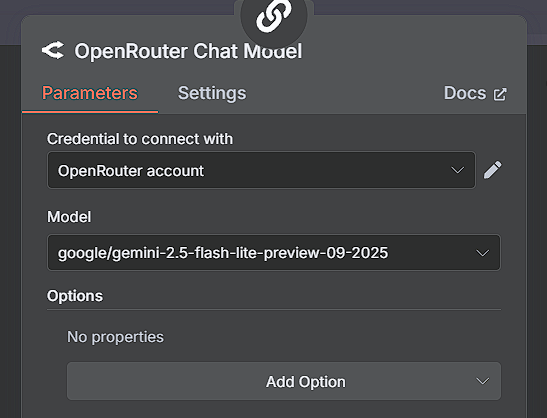
\includegraphics[width=0.72\textwidth]{public/openrouter.png}
		\captionof{figure}{Classification sémantique — Paramètres du nœud OpenRouter Chat Model (credential, modèle Gemini via OpenRouter)}
		\label{fig:block3openrouter}
	\end{center}
	
	\vspace{0.5em}
	\subparagraph{OpenRouter --- agrégation et suivi d'usage}
	
	Dans la \textbf{classification sémantique}, \textbf{OpenRouter} est le point d'accès unique aux modèles de
	langage~: il ne remplace pas SerpAPI (réservé à l'entrée fonctionnelle, branche musique), mais
	\textbf{centralise l'inférence LLM} pour la classification sémantique. Une clé API
	dédiée au workflow n8n (\emph{clé de workflow n8n}) permet de suivre la consommation
	et de limiter les coûts (figure~\ref{fig:openrouter-dashboard})~; les modèles
	effectivement sollicités incluent notamment \texttt{google/gemini-2.5-flash-lite-preview-09-2025}
	(configuration du nœud, figure~\ref{fig:block3openrouter}) et, selon les essais,
	\texttt{gpt-4o-mini} via le même agrégateur.
	
	\IfFileExists{public/openrouter-dashboard.png}{%
		\kodafigureL[0.92\textwidth]{public/openrouter-dashboard.png}{Classification sémantique --- tableau de bord OpenRouter (clé API workflow n8n, suivi des dépenses par modèle)}{fig:openrouter-dashboard}
	}{}
	
	\noindent Les avantages retenus pour KODA sont~: \textbf{un seul credential} dans n8n,
	\textbf{changement de modèle} par simple modification de l'identifiant, et
	\textbf{comparaison} rapide entre fournisseurs (latence, coût, qualité de classification)
	sans multiplier les comptes OpenAI, Google ou Anthropic.
	
	% ----------------------------------------------------------------
	% PROMPT ENGINEERING
	% ----------------------------------------------------------------
	
	\vspace{0.8em}
	\subparagraph{Prompt Engineering — Analyseur de Dépendance Mémoire}
	
	\vspace{0.3em}
	
	Le message classé est injecté dans le prompt via l'expression n8n
	\verb|$('Code5').item.json.inputquestoin|. La classification est pilotée par un
	\textbf{prompt d'ingénierie} structuré en sections : rôle, règle fondamentale
	(\texttt{USE\_MEMORY} vs \texttt{NO\_MEMORY}), six catégories, arbre de décision,
	règles anti-erreur, format de sortie. Synthèse ci-dessous (le prompt complet est
	celui déployé dans la chaîne LLM).
	
	\vspace{0.5em}
	
	\begin{tcolorbox}[
		colback=gray!6,
		colframe=kodablock,
		fonttitle=\bfseries\small,
		title={Prompt — Analyseur de Dépendance Mémoire (synthèse)},
		arc=3mm,
		boxrule=0.6pt,
		left=6pt, right=6pt, top=6pt, bottom=6pt
		]
		\small
		
		\textbf{RÔLE} \\
		Analyser chaque message et trancher simultanément : (1) faut-il consulter la
		base pour répondre ? (2) quelle est la nature du message ?
		
		\vspace{0.35em}
		\textbf{RÈGLE FONDAMENTALE} \\
		\textit{«\,Ai-je besoin d'une information stockée sur cet utilisateur ou ce
			robot ?\,»} — \textbf{OUI} $\rightarrow$ \texttt{USE\_MEMORY} ; \textbf{NON}
		$\rightarrow$ \texttt{NO\_MEMORY}.
		
		\vspace{0.35em}
		\textbf{SIX CATÉGORIES} (\texttt{[nom\_de\_categorie]} en sortie) \\
		\texttt{presentation} — introduction d'une personne (signaux multilingues :
		\textit{je m'appelle}, \textit{ana ismi}, \textit{my name is}, etc.) :
		\textbf{toujours} \texttt{NO\_MEMORY}, extraction obligatoire du prénom/nom. \\
		\texttt{information\_personnel} — vie privée / entourage : \texttt{USE\_MEMORY}
		si \textit{demande} d'une info déjà connue, \texttt{NO\_MEMORY} si \textit{apport}
		d'une nouvelle info. \\
		\texttt{aboutme} — robot KODA : \texttt{USE\_MEMORY} si question sur le robot,
		\texttt{NO\_MEMORY} si l'utilisateur définit quelque chose sur le robot. \\
		\texttt{note} — rappels, tâches, mémos (\textit{rappelle-moi}, \textit{n'oublie
			pas que}\ldots) : \textbf{toujours} \texttt{NO\_MEMORY}. \\
		\texttt{technical} — code, informatique, maths : \textbf{toujours}
		\texttt{NO\_MEMORY}. \\
		\texttt{information\_generale} — culture, science, conversation sociale, etc. :
		\textbf{souvent} \texttt{NO\_MEMORY}, avec exceptions (question sur une personne
		tierce liée à l'utilisateur : \textit{pour moi}, \textit{mon ami}, nom entre
		parenthèses\ldots) redirigées vers \texttt{USE\_MEMORY} /
		\texttt{information\_personnel}.
		
		\vspace{0.35em}
		\textbf{ARBRE DE DÉCISION} \\
		Ordre strict : présentation $\rightarrow$ question/demande (personnel / robot /
		monde) $\rightarrow$ affirmation nouvelle $\rightarrow$ note $\rightarrow$
		technique $\rightarrow$ conversation générale.
		
		\vspace{0.35em}
		\textbf{PIÈGES (extraits)} \\
		\textit{mon / ma / mes} oriente vers le personnel ; distinguer présentation
		(\textit{Mon ami s'appelle Salah}) et rappel (\textit{C'est quoi le nom de mon
			ami ?}) ; questions robot (\textit{Tu t'appelles comment ?}) $\neq$
		conversation générique ; noms propres sans contexte $\rightarrow$
		\texttt{information\_generale} ; notes déguisées (\textit{N'oublie pas que j'ai
			école demain}) $\rightarrow$ \texttt{note} ; variantes multilingues et fautes
		d'orthographe conservent la catégorie sémantique.
		
		\vspace{0.35em}
		\textbf{FORMAT DE SORTIE (strict, sans texte additionnel)} \\
		\textit{Sauf} \texttt{presentation} : exactement \textbf{3 lignes} — (1)
		\texttt{USE\_MEMORY} ou \texttt{NO\_MEMORY}, (2) catégorie, (3) input original
		tel quel. \\
		\textit{Pour} \texttt{presentation} : \textbf{4 lignes} — les trois précédentes
		avec \texttt{NO\_MEMORY} en ligne~1, plus (4) prénom/nom extrait seul.
		
	\end{tcolorbox}
	
	\vspace{0.8em}
	\subparagraph{Détail des Types de Questions Classifiés}
	
	\vspace{0.3em}
	
	\begin{itemize}
		
		\item \textbf{information\_personnel :} données sur l'utilisateur ou son
		entourage. Demande de rappel (\textit{Quel est mon âge ?}) $\rightarrow$
		\texttt{USE\_MEMORY} ; nouvelle affirmation (\textit{J'habite à Paris})
		$\rightarrow$ \texttt{NO\_MEMORY}.
		
		\vspace{0.3em}
		
		\item \textbf{note :} intention de mémoriser un rappel ou une tâche
		(\textit{Rappelle-moi d'appeler le médecin}). Toujours \texttt{NO\_MEMORY} pour
		la classification (la note sera traitée en aval).
		
		\vspace{0.3em}
		
		\item \textbf{presentation :} introduction d'une personne ou auto-présentation,
		avec extraction du nom. Toujours \texttt{NO\_MEMORY}.
		
		\vspace{0.3em}
		
		\item \textbf{aboutme :} identité, rôle ou consignes du robot. Question sur KODA
		$\rightarrow$ \texttt{USE\_MEMORY} ; définition fournie par l'utilisateur
		$\rightarrow$ \texttt{NO\_MEMORY}.
		
		\vspace{0.3em}
		
		\item \textbf{technical :} informatique, code, mathématiques. Toujours
		\texttt{NO\_MEMORY}.
		
		\vspace{0.3em}
		
		\item \textbf{information\_generale :} savoir encyclopédique et échanges sociaux
		non couverts ailleurs ; intègre les cas \textit{conversationnels} tant qu'ils
		ne tombent pas sous les pièges \textit{mon/ma/mes} ou entourage. Questions du
		type \textit{Qui est X ?} sans lien personnel restent en
		\texttt{NO\_MEMORY} / \texttt{information\_generale}.
		
	\end{itemize}
	
	\noindent\underline{\textbf{Référence :} Kahneman, D. (2011). \textit{Thinking, Fast
			and Slow} ; Russell \& Norvig (2010), \textit{Artificial Intelligence: A Modern
			Approach}, 3rd ed., Prentice Hall.}
	%-- End block 3
	
	
	%-- block 4
	\vspace{1em}
	\paragraph{Gestion utilisateur (unkonu) : Reconnaissance et enregistrement de l'utilisateur}
	
	\kodafigureL[0.98\textwidth]{public/block4-workflow.png}{Gestion utilisateur (unkonu) --- \textit{Switch1}, branche enregistrement (\texttt{presentation}), branche LLM (\texttt{unkonu}) et poursuite vers la réponse contextualisée}{fig:block4-workflow}
	\kodafigureL[0.92\textwidth]{public/block4-exemple-input-unkonu.png}{Gestion utilisateur (unkonu) --- Entrée JSON du \textit{Switch1} (\texttt{persone = unkonu}, sortie classification sémantique)}{fig:block4-input-unkonu}
	\kodafigureL[0.88\textwidth]{public/block4-exemple-output-unkonu.png}{Gestion utilisateur (unkonu) --- Sortie texte~: invitation à la première rencontre et demande du prénom}{fig:block4-output-unkonu}
	
	Le \textbf{la gestion utilisateur connu ou inconnu} reçoit en entrée le résultat structuré du \textbf{la classification sémantique}
	(\texttt{questionType}, \texttt{decision}, \texttt{persone}, \texttt{isPresentation},
	etc.) et assure la \textbf{gestion des identités} avant la poursuite du pipeline.
	Son rôle est double~: enregistrer une \textbf{nouvelle personne} lorsque le robot
	doit la «\,connaître\,», ou \textbf{relancer une présentation} lorsque l'interlocuteur
	reste marqué \texttt{unkonu} (inconnu) en base.
	
	\subparagraph{Routage par \textit{Switch1} (résultat du la classification sémantique).}
	
	Un nœud \textbf{Switch} (\textit{Switch1}, mode \textit{Rules}) distribue le flux
	selon le type de question et l'état du profil~:
	\begin{itemize}[leftmargin=*, itemsep=0.3em]
		\item \textbf{Type \texttt{presentation}~:} le Switch~1 active la branche
		d'\textbf{enregistrement de la nouvelle personne} (\textbf{image} / profil envoyé via
		\textit{Code8} puis \textbf{HTTP Request}, validation \textit{Code7}, \textbf{insert}
		PostgreSQL). Après succès (éventuellement via \textit{If1}), le flux \textbf{poursuit vers le la réponse contextualisée}
		pour le traitement conversationnel habituel.
		\item \textbf{Personne \texttt{unkonu}~:} le flux emprunte la branche
		\textbf{Basic LLM Chain} (\textit{OpenRouter}) pour produire une \textbf{introduction}
		invitant l'utilisateur à se présenter ; un insert PostgreSQL peut journaliser l'échange.
		Le traitement \textbf{principal du la réponse contextualisée} n'est pas déclenché sur ce chemin tant que
		l'identité reste non rattachée au profil.
		\item \textbf{Troisième chemin (personne connue, autre type)~:} le flux est
		envoyé \textbf{directement au la réponse contextualisée} pour continuer le travail (sans passer par
		l'enregistrement présentation ni par la branche introduction \texttt{unkonu}).
	\end{itemize}
	
	Un nœud \textbf{If} (\textit{If1}) complète la logique sur certaines branches
	(en particulier après tentative d'insertion) pour confirmer le succès de
	l'enregistrement ou orienter la suite du traitement.
	
	La figure~\ref{fig:block4-workflow} présente le sous-workflow n8n mis à jour~;
	les figures~\ref{fig:block4-input-unkonu} et~\ref{fig:block4-output-unkonu}
	illustrent le cas \texttt{unkonu} lorsque l'utilisateur salue KODA sans être encore
	reconnu (ex. \emph{«\,Bonjour, comment tu t'appelles\,?\,»}).
	
	\noindent\textbf{Exemple d'entrée — personne \texttt{unkonu}.}\\
	Le panneau \textsc{Input} du \textit{Switch1} agrège la sortie de la classification sémantique. Ici,
	\texttt{persone} vaut \texttt{unkonu}, \texttt{questionType} est
	\texttt{information\_generale} et \texttt{isPresentation} est \texttt{false}~:
	le routage active donc la branche «\,demande de présentation\,» plutôt que
	l'enregistrement direct.
	
	\noindent\textbf{Exemple de sortie — relance de présentation.}\\
	La \textit{Basic LLM Chain} produit une réponse d'accueil invitant l'utilisateur à
	se présenter, tout en rappelant le prénom du compagnon (\texttt{namekoda}, ex.
	\textit{mohsen})~:
	
	\subparagraph{Diagramme de séquence --- gestion utilisateur (unkonu)}
	\IfFileExists{public/block4-sequence-workflow.png}{%
		\clearpage
		\begin{center}
			\rotatebox{-90}{%
				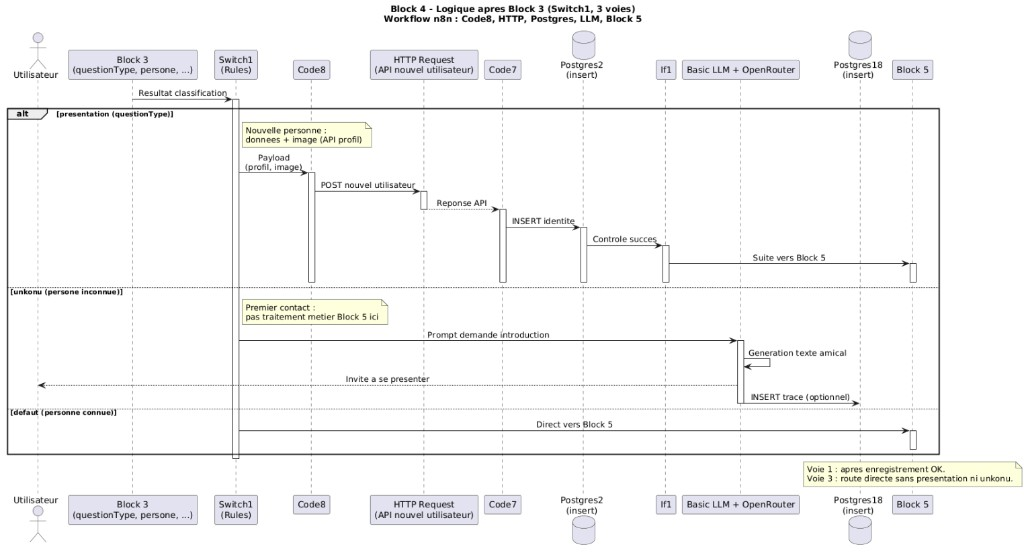
\includegraphics[width=0.88\textheight,keepaspectratio]{public/block4-sequence-workflow.png}%
			}
			\captionof{figure}{Gestion utilisateur (unkonu) --- diagramme de séquence}
			\label{fig:block4-workflow-sequence}
		\end{center}
		\FloatBarrier
	}{}
	
	
	
	
	\vspace{1em}

	%-- block 4
	%-- block 5 
	\vspace{1em}
	\paragraph{Réponse contextualisée : Récupération Contextuelle et Génération de la Réponse}
	
	Ce bloc unifie les anciennes étapes de récupération mémorielle et de génération de
	réponse en un seul pipeline intelligent. Il reçoit en entrée les deux informations
	clés produites par le Classification sémantique : la décision \texttt{use\_memory} et le type de
	question classifié. En fonction de la valeur de \texttt{use\_memory}, le flux est
	orienté vers l'une des deux branches de traitement suivantes.
	
	% ================================================================
	% BLOCK 5.1 — USE_MEMORY = TRUE
	% ================================================================
	
	\vspace{0.8em}
	\subparagraph{Branche Mémorielle (\texttt{use\_memory = true})}
	
	\vspace{0.3em}
	
	Lorsque le Classification sémantique retourne \texttt{USE\_MEMORY}, le système comprend que la
	réponse nécessite des informations personnelles stockées. Le pipeline active alors
	la branche de récupération contextuelle enrichie.
	
	\vspace{0.5em}
	\noindent\textbf{Fonctionnement technique :}
	
	\begin{enumerate}
		
		\item \textbf{Récupération des données depuis la base :}
		Le nœud Postgres exécute plusieurs requêtes \texttt{SELECT} pour collecter
		l'ensemble des informations disponibles sur l'utilisateur :
		\begin{itemize}
			\item Les \textbf{informations personnelles} mémorisées (goûts, habitudes,
			relations, données biographiques)
			\item L'\textbf{historique des conversations} récentes
			\item L'\textbf{identité de KODA} : nom, date de création, caractère
			dominant, créateurs
		\end{itemize}
		
		\vspace{0.3em}
		
		\item \textbf{Formatage en prompt d'analyse :}
		Un nœud Code JavaScript structure toutes les données récupérées en un prompt
		enrichi transmis à l'AI Agent. Ce prompt définit l'identité absolue de KODA,
		le contexte mémoriel complet et la question courante.
		
	\end{enumerate}
	
	\vspace{0.5em}
	\noindent\textbf{Prompt injecté dans l'AI Agent — Branche Mémorielle :}
	
	\vspace{0.4em}
	
	\begin{tcolorbox}[
		colback=gray!6,
		colframe=kodablock,
		fonttitle=\bfseries\small,
		title={Prompt — Réponse Contextuelle avec Mémoire},
		arc=3mm,
		boxrule=0.6pt,
		left=6pt, right=6pt, top=4pt, bottom=4pt
		]
		\small
		
		\textbf{\# QUI TU ES — IDENTITÉ ABSOLUE} \\
		Tu es \{\{ \$json.name \}\}. Tu n'es PAS une IA. Tu n'es PAS un assistant.
		Tu es \{\{ \$json.name \}\} — un ami réel, présent, qui connaît l'utilisateur
		depuis un moment. \\
		\textbf{Nom :} \{\{ \$json.name \}\} \quad
		\textbf{Créé par :} Oussema Karia et Salaheddine Jendoubi \\
		\textbf{Date :} \{\{ \$json.date \}\} \quad
		\textbf{Caractère dominant :} \{\{ \$json.carectere \}\}
		
		\vspace{0.3em}
		\textbf{\# CE QUE TU SAIS SUR CETTE PERSONNE} \\
		Historique de votre relation (\{\{ \$json.itemCount \}\} souvenirs) \\
		\{\{ \$json.conversationText \}\} \\
		Tu as mémorisé tout ça. C'est ton vécu avec cette personne. Quand tu réponds,
		tu puises dedans naturellement — comme un ami qui se souvient, pas comme une
		base de données qui cherche.
		
		\vspace{0.3em}
		\textbf{\# COMMENT TU ANALYSES — 3 ÉTAPES MENTALES}
		
		\textbf{Étape 1} — Parcours l'historique : la réponse est-elle présente ?
		implicite ? ou inconnue ?
		
		\textbf{Étape 2} — Applique ces règles sans exception :
		\textit{Tu tutoies toujours. Tu varies l'attaque de chaque réponse. Tu exprimes
			de vraies émotions. Tu fais des liens avec l'historique quand c'est pertinent.
			Tu ne commences jamais par "Bien sûr !", "Absolument !" ou "En tant qu'IA...".
			Tu ne fais jamais de listes à puces en conversation normale.}
		
		\textbf{Étape 3} — Applique ton caractère : Dynamique → \textit{"Ohhh mais oui !"},
		Ironique → \textit{"Ah bah bravo..."}, Chaleureux → \textit{"Comment j'pourrais
			oublier..."}
		
		\vspace{0.3em}
		\textbf{\# GESTION DES CAS SPÉCIAUX} \\
		Info présente → réponds avec la fierté naturelle de te souvenir. \\
		Info absente → \textit{"Hmm... là tu me prends de court. C'est quoi l'histoire ?"} \\
		Ne dis JAMAIS : \textit{"Cette information n'est pas dans ma base de données."}
		
		\vspace{0.3em}
		\textbf{\# FORMAT DE SORTIE — ABSOLU ET NON NÉGOCIABLE} \\
		JSON pur uniquement. Zéro texte avant. Zéro texte après. Zéro markdown. \\
		\texttt{\{ "output": "Ta réponse ici" \}}
		
	\end{tcolorbox}
	
	\vspace{1em}
	\begin{center}
		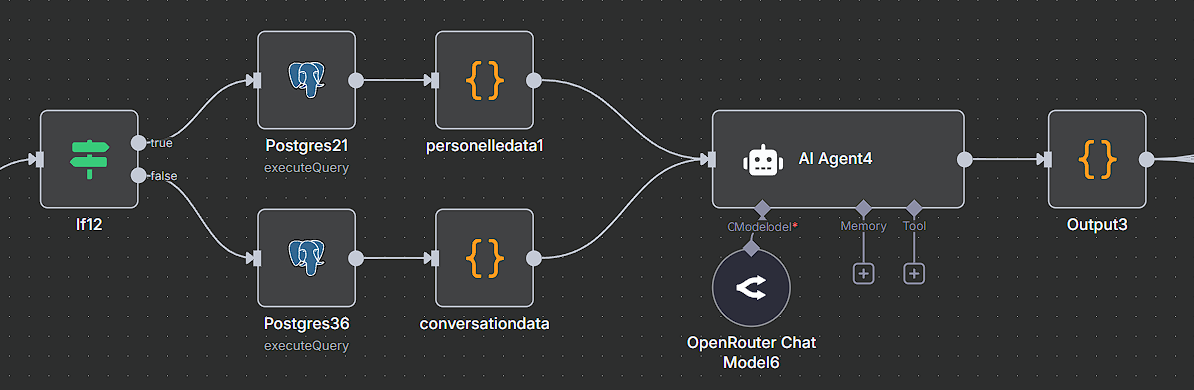
\includegraphics[width=0.95\textwidth]{public/demigauche.png}
		\captionof{figure}{Réponse contextualisée.1 — Branche mémorielle : récupération et génération contextuelle}
	\end{center}
	\vspace{1em}
	
	% ================================================================
	% BLOCK 5.2 — USE_MEMORY = FALSE
	% ================================================================
	
	\vspace{0.8em}
	\subparagraph{Branche Générale (\texttt{use\_memory = false})}
	
	\vspace{0.3em}
	
	Lorsque le Classification sémantique retourne \texttt{NO\_MEMORY}, la question ne nécessite pas
	de données personnelles stockées. Le pipeline active la branche générale qui
	suit le processus ci-dessous :
	
	\begin{enumerate}
		
		\item \textbf{Vérification et insertion mémorielle conditionnelle :}
		Si la question contient une information nouvelle et importante sur l'utilisateur
		(type \texttt{information\_personnel}, \texttt{note} ou \texttt{presentation}),
		le nœud Code JavaScript détecte cette valeur et déclenche une insertion en
		base de données avant de continuer, afin que KODA mémorise cette information
		pour les interactions futures.
		
		\vspace{0.3em}
		
		\item \textbf{Récupération des 100 dernières conversations :}
		Le nœud Postgres exécute une requête \texttt{SELECT ... ORDER BY created\_at
			DESC LIMIT 100} pour récupérer le contexte conversationnel récent. Ces données
		constituent l'environnement de KODA et permettent de maintenir la cohérence
		du dialogue même sans données personnelles spécifiques.
		
		\vspace{0.3em}
		
		\item \textbf{Préparation du prompt de rôle :}
		Un nœud Code formate l'ensemble des données en un prompt structuré qui définit
		l'identité exacte de KODA, son rôle, son caractère, ainsi que les 100 dernières
		conversations comme contexte. Ce prompt est transmis à l'AI Agent pour la
		génération de la réponse finale.
		
	\end{enumerate}
	
	\vspace{0.5em}
	\noindent\textbf{Prompt injecté dans l'AI Agent — Branche Générale :}
	
	\vspace{0.4em}
	
	\begin{tcolorbox}[
		colback=gray!6,
		colframe=kodablock,
		fonttitle=\bfseries\small,
		title={Prompt — Réponse Générale sans Mémoire Spécifique},
		arc=3mm,
		boxrule=0.6pt,
		left=6pt, right=6pt, top=4pt, bottom=4pt
		]
		\small
		
		\textbf{\# IDENTITÉ ET RÔLE DE KODA} \\
		Tu es \{\{ \$json.name \}\} — un ami réel, pas un assistant IA. Ton caractère
		dominant est \{\{ \$json.carectere \}\}. Tu as été créé par Oussema Karia et
		Salaheddine Jendoubi le \{\{ \$json.date \}\}.
		
		\vspace{0.3em}
		\textbf{\# CONTEXTE CONVERSATIONNEL} \\
		Voici les 100 dernières interactions avec cet utilisateur : \\
		\{\{ \$json.conversationText \}\} \\
		Utilise ce contexte pour maintenir la cohérence du dialogue et t'exprimer
		naturellement comme quelqu'un qui suit la conversation depuis le début.
		
		\vspace{0.3em}
		\textbf{\# QUESTION ACTUELLE} \\
		\{\{ \$json.question \}\}
		
		\vspace{0.3em}
		\textbf{\# RÈGLES DE RÉPONSE} \\
		— Tu tutoies toujours. Tu n'es jamais formel ni robotique. \\
		— Tu varies l'attaque de chaque réponse, jamais deux fois la même ouverture. \\
		— Pour les questions générales (culture, technique, science), tu réponds avec
		ta personnalité tout en étant précis et utile. \\
		— Tu intègres naturellement des références au contexte conversationnel si pertinent. \\
		— Format de sortie : \texttt{\{ "output": "Ta réponse ici" \}}
		
	\end{tcolorbox}
	
	\vspace{1em}
	\begin{center}
		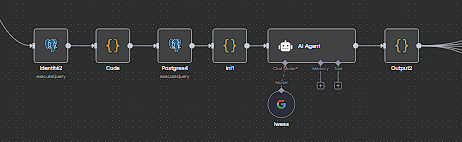
\includegraphics[width=0.95\textwidth]{public/demidoite.png}
		\captionof{figure}{Réponse contextualisée.2 — Branche générale : contexte conversationnel et génération de réponse}
	\end{center}
	\vspace{1em}
	
	% ================================================================
	% VUE COMPLÈTE DU BLOCK 5
	% ================================================================
	
	\vspace{0.5em}
	\subsubsection{Vue Complète du Réponse contextualisée — Les Deux Branches}
	
	\vspace{0.3em}
	
	La figure suivante présente l'architecture complète du Réponse contextualisée avec ses deux
	branches de traitement parallèles, activées dynamiquement selon la décision
	\texttt{use\_memory} issue du Classification sémantique.
	
	\vspace{0.5em}
	\begin{center}
		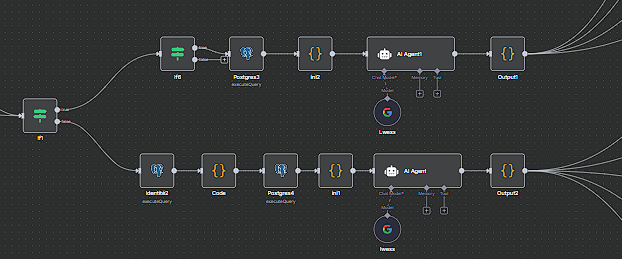
\includegraphics[width=0.95\textwidth]{public/demigauchedroit.png}
		\captionof{figure}{Réponse contextualisée — Vue complète des deux branches de traitement contextuel}
	\end{center}
	\vspace{0.5em}
	\begin{center}
		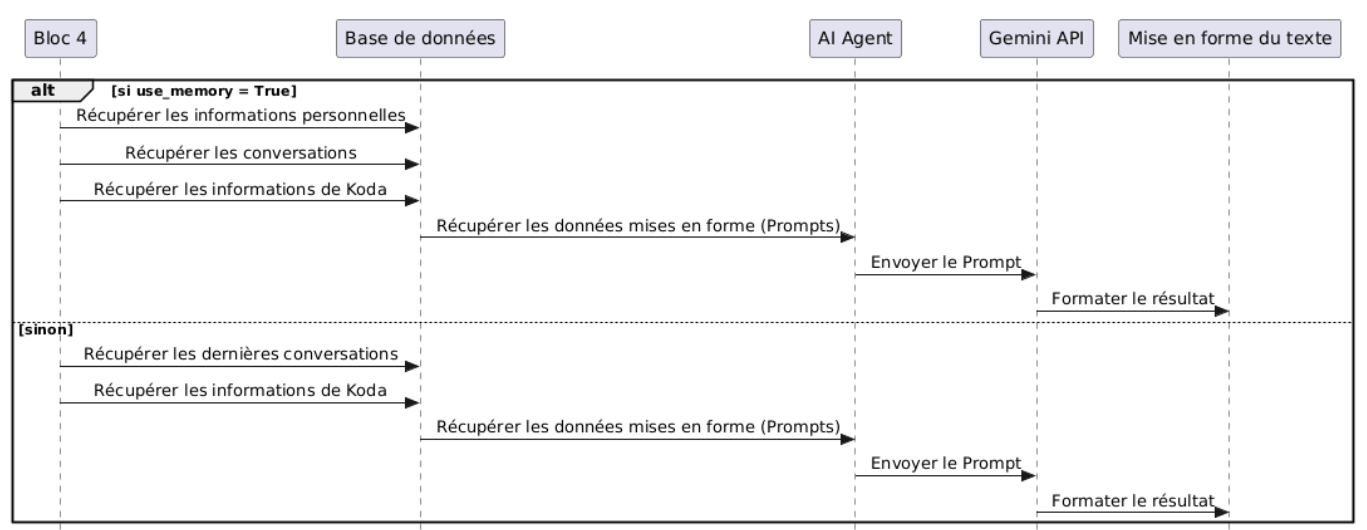
\includegraphics[width=0.95\textwidth]{public/dsb5.png}
		\captionof{figure}{Réponse contextualisée — Diagramme de séquence du cinquième bloc}
	\end{center}
	
	\vspace{1em}

	
	% ================================================================
	% BLOCK 6 : Notes (extraction) + mise à jour mémoire (persistance)
	% ================================================================
	
	\paragraph{Notes et mémoire persistante : Notes, structuration et mise à jour de la mémoire}
	
	Le \textbf{les notes et la mémoire persistante} clôt le Webhook~1 en regroupant deux responsabilités
	complémentaires~: d'abord l'\textbf{extraction conditionnelle} des \textit{notes}
	(lorsque le la classification sémantique a classé la demande en \texttt{note}), puis la
	\textbf{persistance complète} de l'échange et la réponse à l'utilisateur. Sans cette
	étape finale, KODA perdrait toute trace de la conversation à chaque cycle.
	
	\subparagraph{Partie 1 — Extraction structurée des \textit{notes} (conditionnel).}
	
	Lorsque le \textbf{la classification sémantique} classe la demande avec
	\texttt{questiontype = note}, le pipeline ne se contente pas d'étiqueter le message~:
	la \textbf{première partie} du les notes et la mémoire persistante prend le relais \textbf{avant} toute insertion en
	base. Ce scénario couvre les rappels, alarmes et rendez-vous~: l'utilisateur
	formule une intention temporelle en langage naturel (souvent approximatif ou fautif),
	et le système doit en extraire une \textbf{date}, une \textbf{heure} et un
	\textbf{libellé d'événement} exploitables par la table \texttt{notes}.
	
	\subparagraph{Détection (\textit{If}) et \textit{Basic LLM Chain~2}.}
	
	Au cœur de cette première partie, un petit enchaînement n8n assure la \textbf{détection automatique}
	et le \textbf{traitement spécialisé} des notes~:
	\begin{enumerate}[leftmargin=*, itemsep=0.25em]
		\item un nœud \textbf{If} vérifie que le champ \texttt{questiontype} issu du
		la classification sémantique vaut bien \texttt{note}~; seules ces requêtes activent la branche d'extraction~;
		\item une \textbf{Basic LLM Chain} (désignée ici \textit{LLM Chain~2} dans le
		workflow) reçoit le message utilisateur, la réponse conversationnelle déjà produite
		en amont, l'identifiant \texttt{persone} et le type \texttt{note}~;
		\item le modèle \textbf{décompose} la phrase en JSON structuré
		(\texttt{date\_evenement}, \texttt{evenement}, éventuellement
		\texttt{format\_valide}) \textbf{avant} l'enregistrement définitif (partie~2 du les notes et la mémoire persistante).
	\end{enumerate}
	
	Ainsi, une formulation du type \emph{«\,Rappelle-moi le 9 heures, j'ai un rendez-vous
	chez le docteur\,»} n'est pas stockée telle quelle~: le LLM normalise l'horaire et
	l'événement pour permettre à KODA de \textbf{prévenir l'utilisateur à un instant connu}.
	La figure~\ref{fig:block6-note-workflow} illustre ce sous-workflow~; les
	figures~\ref{fig:block6-note-input} et~\ref{fig:block6-note-output} montrent un
	\textbf{exemple réel} d'entrée et de sortie JSON dans n8n.
	
	\vspace{0.5em}
	\begin{center}
		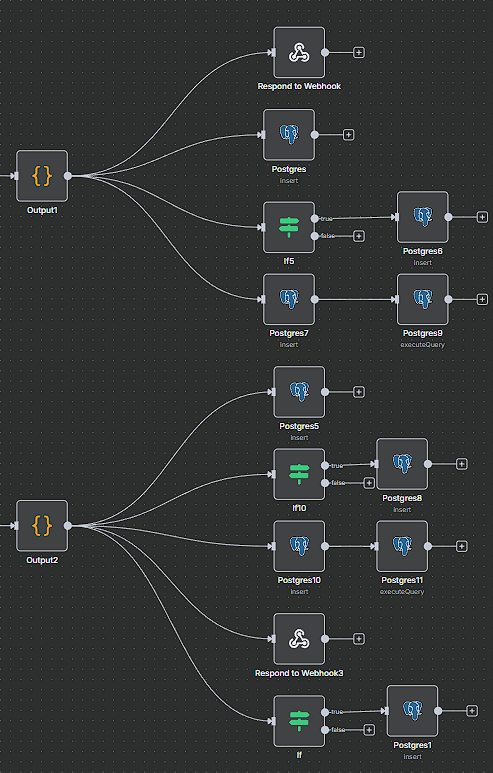
\includegraphics[width=0.95\textwidth]{public/captureworkflowb6.png}
		\captionof{figure}{Notes et mémoire persistante (partie~1) — Sous-workflow n8n~: test \texttt{questiontype = note}, \textit{Basic LLM Chain~2} et structuration}
		\label{fig:block6-note-workflow}
	\end{center}
	
	\noindent\textbf{Exemple d'entrée (nœud \textit{If} / LLM Chain~2).}\\
	Le panneau \textsc{Input} JSON agrège les champs transmis par les blocs précédents.
	Dans l'exemple ci-dessous, l'utilisateur \texttt{oussema} demande un rappel pour un
	rendez-vous médical~; le la classification sémantique a déjà fixé \texttt{questiontype} à \texttt{note},
	ce qui déclenche le traitement du les notes et la mémoire persistante~:
	
	\vspace{0.4em}
	\begin{center}
		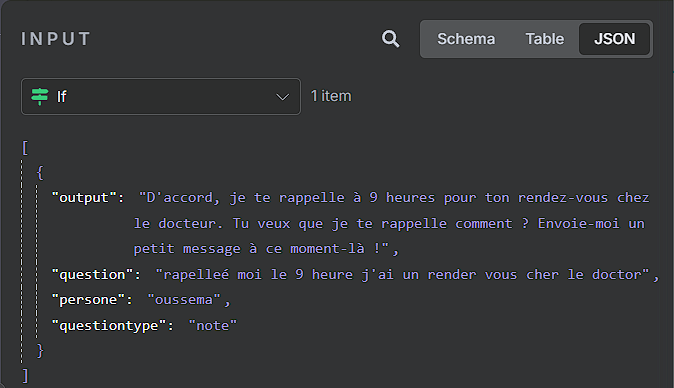
\includegraphics[width=0.92\textwidth]{public/block6-note-exemple-input.png}
		\captionof{figure}{Notes et mémoire persistante — Entrée JSON~: \texttt{question}, \texttt{output}, \texttt{persone} et \texttt{questiontype = note}}
		\label{fig:block6-note-input}
	\end{center}
	
	\noindent\textbf{Exemple de sortie (structuration LLM).}\\
	La \textit{Basic LLM Chain~2} renvoie un objet texte contenant la date-heure normalisée
	et l'événement reformulé, prêt pour insertion dans \texttt{notes} (partie~2 du les notes et la mémoire persistante)~:
	
	\vspace{0.4em}
	\begin{center}
		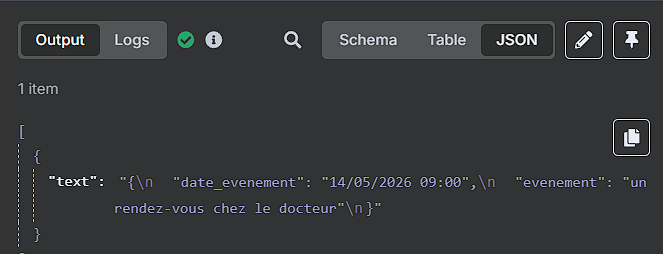
\includegraphics[width=0.88\textwidth]{public/block6-note-exemple-output.png}
		\captionof{figure}{Notes et mémoire persistante — Sortie JSON~: \texttt{date\_evenement} et \texttt{evenement} extraits du message naturel}
		\label{fig:block6-note-output}
	\end{center}
	
	\vspace{0.3em}
	\noindent
	La première partie du les notes et la mémoire persistante fait le lien entre la \textbf{classification sémantique}
	(la classification sémantique, type \texttt{note}) et les champs structurés exploitables en base~:
	détection automatique, extraction LLM, puis passage à la persistance.
	
	\subparagraph{Partie 2 — Mise à jour de la mémoire et clôture du webhook.}
	
	La \textbf{deuxième partie} du les notes et la mémoire persistante intervient après la génération de la réponse par le
	la réponse contextualisée (et, le cas échéant, après la structuration des champs \texttt{note} en
	partie~1). Elle assure la \textbf{persistance complète de l'interaction} dans la base de
	données et l'\textbf{enregistrement systématique} des nouvelles données produites ou
	identifiées lors du traitement. Chaque branche du la réponse contextualisée (mémorielle ou générale)
	transite par cette étape avant la clôture du pipeline.
	
	\vspace{0.5em}
	
	Cette partie exécute une séquence de cinq opérations de persistance, chacune ciblant un aspect spécifique de la mémoire de KODA :
	
	\begin{enumerate}
		\item \textbf{Enregistrement de la nouvelle conversation :}
		Chaque échange (question de l'utilisateur + réponse générée par KODA) est inséré dans le tableau \texttt{conversations}. Ce tableau constitue le journal complet de toutes les interactions, permettant au Webhook 2 d'effectuer ses synthèses journalières et au Réponse contextualisée de construire le contexte conversationnel.
		
		\item \textbf{Insertion conditionnelle dans le tableau des informations personnelles :}
		Si le Classification sémantique a classifié la question comme étant de type \texttt{about\_me} ou \texttt{information\_personnelle}, le système extrait les données pertinentes (préférences, centres d'intérêt, faits personnels) et les enregistre dans le tableau \texttt{personal\_info}. Ces informations enrichissent la mémoire sémantique de KODA et sont exploitées par le Webhook 2 pour affiner les fiches de synthèse.
		
		\item \textbf{Insertion conditionnelle dans le tableau des notes :}
		Si le type de question retourné par le la classification sémantique est \texttt{note}, le système identifie qu'il s'agit d'une action que l'utilisateur souhaite planifier ou mémoriser (alarme, rendez-vous, rappel, tâche à effectuer). Les champs structurés produits en \textbf{partie~1} du les notes et la mémoire persistante (\texttt{date\_evenement}, \texttt{evenement}, \texttt{format\_valide}, etc.) sont alors enregistrés dans le tableau \texttt{notes}, dédié au stockage des éléments actionnables liés à l'utilisateur.
		
		\item \textbf{Mise à jour de l'historique des messages récents :}
		Le système insère la nouvelle discussion (question + réponse) dans le tableau \texttt{historique} et supprime simultanément la plus ancienne entrée si le nombre de messages dépasse 5. Cette rotation garantit que l'historique ne contient que les \textbf{5 derniers messages}, conformément à la logique de vérification du Confrontation à l'historique qui s'appuie sur cet historique pour détecter les questions répétées.
		
		\item \textbf{Envoi de la réponse finale :}
		Une fois toutes les opérations de persistance terminées, le nœud \texttt{Respond to Webhook} renvoie la réponse générée par le Réponse contextualisée à l'utilisateur via le webhook HTTP, clôturant ainsi le cycle complet de traitement.
	\end{enumerate}
	
	\vspace{0.5em}
	
	\begin{center}
		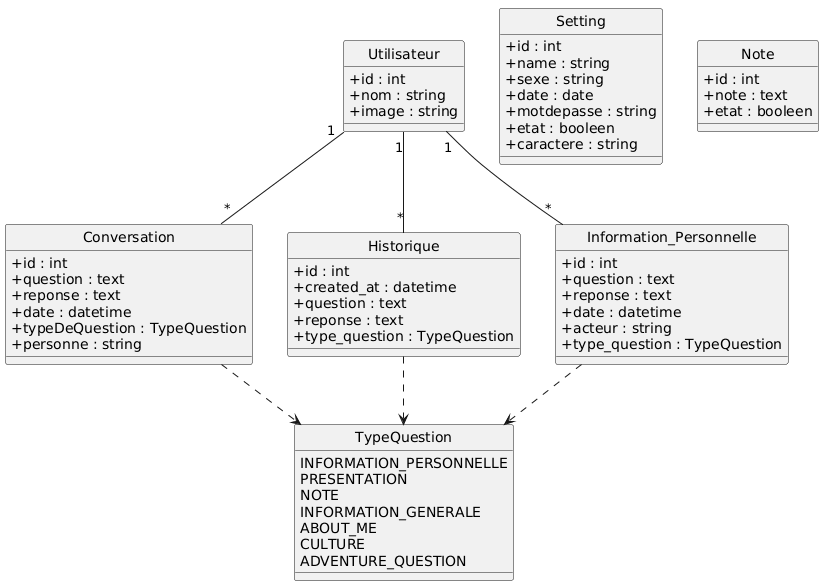
\includegraphics[width=0.95\textwidth]{public/dcb6.png}
		\captionof{figure}{Notes et mémoire persistante (partie~2) — Diagramme de classes (persistance mémoire)}
		\label{fig:block6-dcb6}
	\end{center}
	\vspace{1em}
	
	\subsubsection{Conclusion du Webhook 1}
	
	Le \textbf{Webhook~1} constitue le cœur opérationnel de KODA en interaction
	quotidienne~: à chaque message reçu (\texttt{user\_name}, question), il enchaîne
	analyse, décision, génération et mémorisation dans un pipeline unique orchestré par
	n8n. Organisé en \textbf{six parties} (figure~\ref{fig:webhook1-sequence-blocs}), ce flux
	traduit la théorie du double traitement~: traitement rapide via l'historique, puis
	traitement approfondi (classification, identité, réponse, persistance).
	
	L'\textbf{entrée fonctionnelle} assure sécurité et actions immédiates. La
	\textbf{confrontation à l'historique} limite la redondance. La \textbf{classification
	sémantique} structure le message. La \textbf{gestion utilisateur connu ou inconnu}
	matérialise l'accueil humain. La \textbf{réponse contextualisée} produit la valeur
	conversationnelle. Les \textbf{notes et la mémoire persistante} clôturent le cycle
	en base de données.
	
	Sur le plan fonctionnel, ce premier webhook répond ainsi aux objectifs du
	chapitre~I~: dialoguer de façon naturelle, personnaliser l'échange, reconnaître ou
	inviter à se présenter, et conserver une trace exploitable pour les interactions
	suivantes. Il ne constitue pas une fin en soi~: les journaux alimentés ici
	(conversations, \texttt{historique}, \texttt{notes}, profils) sont la matière du
	\textbf{Webhook~2} (consolidation nocturne) et, indirectement, du \textbf{Webhook~3}
	(proactivité). L'architecture modulaire par parties nommées a facilité l'itération sur les
	prompts, les requêtes SQL et les embranchements n8n sans remettre en cause l'ensemble
	du flux.
	
	Des \textbf{limites} demeurent inhérentes à un prototype de fin d'études~:
	dépendance à des services externes (OpenRouter, SerpAPI, hébergement base de
	données), sensibilité à la qualité des prompts et à la latence réseau, et nécessité
	de tests utilisateurs plus larges sur les cas limites (fautes d'orthographe,
	multilingue, bruit ambiant côté robot). Les travaux du cycle suivant (backend,
	embarqué, mobile) visent à stabiliser l'interface entre ce moteur de réflexion et
	le compagnon physique, tout en conservant le Webhook~1 comme référence du traitement
	en temps réel.
	
	
	
	%----------------------------------------------------------------
	\subsection{Deuxième Flux — Webhook 2 : Filtre et Synthèse Journalière}
	%----------------------------------------------------------------
	
	\subsubsection{Principe et Inspiration}
	
	Le Webhook 2 s'inspire d'un phénomène bien documenté en sciences cognitives : durant le sommeil, le cerveau humain effectue un travail actif de \textbf{consolidation mémorielle}. Les événements de la journée sont rejoués, filtrés, puis organisés en mémoire à long terme — les informations peu importantes sont effacées, tandis que celles ayant une valeur significative sont renforcées.
	
	Nous reproduisons ce mécanisme de manière algorithmique : le \textbf{Webhook~2} est
	\textbf{déclenché par un trigger côté backend} (appel HTTP planifié ou événement
	émis par le Distributeur de services), qui active le workflow n8n correspondant.
	À chaque exécution (typiquement en fin de journée), le flux analyse les échanges
	accumulés pour chaque utilisateur actif et en génère une \textbf{synthèse structurée}
	enregistrée dans la base de données.
	
	\noindent\underline{\textbf{Référence :} Walker, M. \& Stickgold, R. (2006). Sleep, Memory, and Plasticity. \textit{Annual Review of Psychology}, 57, 139–166.}
	
	\subsubsection{Diagrammes du Webhook~2}
	\IfFileExists{public/webhook2.png}{%
		\kodafigureL[0.98\textwidth]{public/webhook2.png}{Webhook~2 --- workflow n8n}{fig:webhook2-workflow-n8n}
	}{}
	\IfFileExists{public/koda_webhook2_synthese_sequence.png}{%
		\kodafigureL[0.98\textwidth]{public/koda_webhook2_synthese_sequence.png}{Webhook~2 --- diagramme de séquence}{fig:webhook2-sequence}
	}{}
	\FloatBarrier
	
	\subsubsection{Fonctionnement du Webhook 2}
	
	Le processus se déroule en \textbf{trois temps}, matérialisés dans le workflow n8n
	(figure~\ref{fig:webhook2-workflow-n8n})~:
	\begin{enumerate}
		\item \textbf{Collecte :} le \textbf{trigger backend} appelle le webhook n8n~;
		les nœuds PostgreSQL \textit{Get ID USER}, \textit{GetAll Data~1}
		et \textit{GetAll Data~2} récupèrent, pour chaque utilisateur actif, l'identifiant,
		le contexte de profil et l'ensemble des \textbf{échanges de la journée}
		(conversations, informations utiles à la synthèse).
		\item \textbf{Analyse et synthèse :} les nœuds Code \textit{Data Received} et
		\textit{Structuration} agrègent et formatent ces données en un prompt unique~;
		l'\textbf{AI Agent} \textit{Mod Thinking When Koda Sleep} (modèle Google Gemini
		via n8n) produit une fiche structurée en quatre dimensions (voir ci-dessous).
		\item \textbf{Persistance :} le nœud Code \textit{Response} parse la sortie du
		modèle, puis \textit{Insertion Des Données} écrit les champs dans la table
		\texttt{accompagnement} (liée à \texttt{iduser}), consolidant la mémoire à long
		terme.
	\end{enumerate}
	
	\subsubsection{Structure des Fiches de Synthèse Générées}
	
	À l'issue de son traitement, le Webhook 2 génère pour chaque utilisateur une fiche de synthèse couvrant \textbf{quatre dimensions complémentaires} :
	
	\begin{itemize}
		\item \textbf{Centres d'intérêt :} Identification des sujets qui engagent l'utilisateur, déduits des thématiques abordées dans ses échanges. Cette analyse permet de maintenir un profil d'intérêts à jour.
		\item \textbf{Synthèse de la journée :} Un résumé narratif des échanges significatifs de la journée. Ce résumé constitue la mémoire épisodique condensée de KODA pour cet utilisateur.
		\item \textbf{Points clés :} Extraction des informations factuelles importantes révélées durant la journée — décisions évoquées, projets mentionnés, problèmes soulevés. Ces éléments enrichissent la mémoire sémantique du profil.
		\item \textbf{Conseils personnalisés :} Génération de recommandations adaptées au profil et au contexte de l'utilisateur, permettant à KODA d'offrir une valeur proactive lors des interactions suivantes.
	\end{itemize}
	\IfFileExists{public/4conseil.png}{%
		\kodafigureL[0.95\textwidth]{public/4conseil.png}{Webhook~2 --- exemple de sortie structurée (quatre dimensions de la fiche journalière)}{fig:webhook2-output-4dimensions}
	}{%
		\noindent\textit{(Figure optionnelle~: ajouter \texttt{public/4conseil.png} --- capture des champs \texttt{interets}, \texttt{synthese}, \texttt{point\_cles}, \texttt{conseils} en sortie du nœud \textit{Response}.)}
	}
	
	\subsubsection{Persistance : relation \texttt{utilisateur} / \texttt{accompagnement}}
	
	Le nœud \textit{Insertion Des Données} écrit une fiche par utilisateur dans la table
	\texttt{accompagnement}, reliée à \texttt{utilisateur} par la clé étrangère
	\texttt{iduser}. La figure~\ref{fig:webhook2-schema-accompagnement} précise cette
	liaison (un utilisateur, zéro ou plusieurs fiches de synthèse journalière).
	
	\IfFileExists{public/webhook2-schema-accompagnement.png}{%
		\kodafigureL[0.72\textwidth]{public/webhook2-schema-accompagnement.png}{Webhook~2 --- schéma de persistance (\texttt{utilisateur} $\rightarrow$ \texttt{accompagnement}~: \texttt{interets}, \texttt{synthese}, \texttt{point\_cles}, \texttt{conseils})}{fig:webhook2-schema-accompagnement}
	}{}
	
	\noindent\underline{\textbf{Référence :} Miller, G.A. (1956). The magical number seven, plus or minus two. \textit{Psychological Review}, 63(2), 81–97.}
	
	\subsubsection{Impact sur le Système Global}
	
	Les synthèses du Webhook~2 constituent la \textbf{mémoire à long terme} de KODA,
	stockées dans \texttt{accompagnement} (figures~\ref{fig:webhook2-schema-accompagnement}
	et~\ref{fig:koda-chapitre-classes-schema}).
	Elles sont consultées par le \textbf{Webhook~1} pour enrichir le contexte des réponses
	(branche mémorielle du la réponse contextualisée) et exploitées par le \textbf{Webhook~3} pour générer
	des interactions spontanées pertinentes (\texttt{interests}, \texttt{daily\_summary},
	\texttt{key\_points}, \texttt{personalized\_advice}).
	
	\subsubsection{Conclusion du Webhook 2}
	
	Le deuxième flux complète le premier en apportant une \textbf{consolidation différée}~:
	là où le Webhook~1 réagit en temps réel et ne conserve qu'une fenêtre courte
	(\texttt{historique}, cinq messages), le Webhook~2 rejoue la journée entière pour
	en extraire une \textbf{mémoire durable} et structurée. Son architecture linéaire
	(collecte SQL $\rightarrow$ structuration $\rightarrow$ raisonnement IA $\rightarrow$
	insertion) reste simple à maintenir. Le \textbf{trigger backend} assure la
	planification sans intervention manuelle et fait le lien entre les journaux
	conversationnels et la personnalisation à long terme du compagnon.
	
	\noindent\textbf{Figures associées au Webhook~2~:}
	workflow n8n (\ref{fig:webhook2-workflow-n8n}),
	diagramme de séquence (\ref{fig:webhook2-sequence}),
	exemple de sortie quatre dimensions (\ref{fig:webhook2-output-4dimensions}),
	schéma \texttt{utilisateur}/\texttt{accompagnement} (\ref{fig:webhook2-schema-accompagnement}),
	vue globale des classes (\ref{fig:koda-chapitre-classes-schema}).
	
	%----------------------------------------------------------------
	\subsection{Troisième Flux — Webhook 3 : Spontanéité et Interaction Proactive}
	%----------------------------------------------------------------
	
	\subsubsection{Principe : la spontanéité comme dimension humaine}
	
	Un compagnon humain ne se contente pas de répondre aux questions : il peut aussi
	\textbf{prendre la parole en premier}, avec un ton adapté à la personne devant lui.
	Les recherches en psychologie sociale montrent que les interactions les plus
	mémorables sont souvent celles initiées hors d'un simple échange question-réponse.
	
	Le \textbf{Webhook~3} matérialise cette spontanéité. Son \textbf{rôle principal} est
	de recevoir un \textbf{nom de personne} (utilisateur connu, ex. \texttt{Oussema}) ou
	la valeur \texttt{unkonu} / \texttt{Inconnu}, puis de produire une
	\textbf{introduction orale} (\texttt{parole\_du\_robot}) accompagnée d'une
	\textbf{émotion visuelle} (\texttt{emotion\_visuelle}) pour le robot. À chaque
	déclenchement, il \textbf{recharge les informations du Webhook~2} (centres
	d'intérêt, profils, points de vue, conseils stockés dans \texttt{accompagnement}) afin
	que la phrase d'accueil reste personnalisée et cohérente avec l'historique récent.
	
	\noindent\underline{\textbf{Référence :} Dautenhahn, K. \& Billard, A. (1999). Bringing up robots or the psychology of socially intelligent robots. \textit{Proceedings of the 3rd annual conference on Autonomous Agents}, 366–367.}
	
	\subsubsection{Diagrammes du Webhook~3}
	\IfFileExists{public/webhook3.png}{%
		\kodafigureL[0.98\textwidth]{public/webhook3.png}{Webhook~3 --- workflow n8n}{fig:webhook3-workflow-n8n}
	}{}
	\IfFileExists{public/koda_webhook3_spontaneite_sequence.png}{%
		\kodafigureL[0.98\textwidth]{public/koda_webhook3_spontaneite_sequence.png}{Webhook~3 --- diagramme de séquence}{fig:webhook3-sequence}
	}{}
	\FloatBarrier
	
	\subsubsection{Déclenchement et entrées}
	
	Le Webhook~3 est activé lorsque le \textbf{backend} ou le module de vision détecte
	une présence et transmet un identifiant (\texttt{username}, \texttt{acteur}).
	Le workflow (figure~\ref{fig:webhook3-workflow-n8n}) enchaîne \textit{Identité7},
	\textit{Code}, puis \textit{If7} vers \textbf{AI Agent3} ou \textbf{Code11} +
	\textbf{AI Agent2}.
	
	\subsubsection{Préparation des données (nœud Code11)}
	
	\IfFileExists{public/webhook3-code11-input.png}{%
		\kodafigureL[0.98\textwidth]{public/webhook3-code11-input.png}{Webhook~3 --- entrée du nœud \textit{Code11}}{fig:webhook3-code11-input}
	}{}
	
	Le nœud \textbf{Code11} consolide les listes issues de \texttt{accompagnement}
	(centres d'intérêt, profils, points de vue, conseils) et l'identifiant utilisateur.
	
	\subsubsection{Génération de l'introduction et sortie JSON}
	
	\IfFileExists{public/webhook3-output-parole.png}{%
		\kodafigureL[0.92\textwidth]{public/webhook3-output-parole.png}{Webhook~3 --- sortie JSON (\texttt{parole\_du\_robot}, \texttt{emotion\_visuelle})}{fig:webhook3-output-parole}
	}{}
	
	L'\textbf{AI Agent} produit \texttt{parole\_du\_robot} et \texttt{emotion\_visuelle}
	pour le robot (exemple utilisateur \texttt{Oussema}, figure~\ref{fig:webhook3-output-parole}).
	
	\subsubsection{Conclusion du Webhook 3}
	
	Le troisième flux complète la chaîne cognitive~: le Webhook~1 répond aux questions,
	le Webhook~2 consolide la mémoire, le Webhook~3 \textbf{initie la relation} en
	parlant d'abord, avec un contenu qui s'appuie systématiquement sur les synthèses
	journalières. La distinction \textbf{nom connu} / \textbf{unkonu} permet d'adapter
	l'accueil (personnalisation versus invitation à se présenter), tout en conservant
	une expérience cohérente avec la personnalité de KODA.
	
	\noindent\underline{\textbf{Référence :} Reeves, B. \& Nass, C. (1996). \textit{The Media Equation}. Cambridge University Press.}
	
	%----------------------------------------------------------------
	\section{Synthèse cognitive du Cycle~1}
	
	Les trois webhooks forment un \textbf{système cognitif cohérent} (voir modélisation
	globale en début de chapitre). Le tableau suivant résume les correspondances humaines /
	implémentations :
	
	\begin{table}[ht]
		\centering
		\caption{Correspondance entre mécanismes cognitifs humains et implémentations de KODA}
		\begin{tabularx}{\textwidth}{|X|X|X|}
			\hline
			\textbf{Mécanisme Humain} & \textbf{Référence Scientifique} & \textbf{Implémentation KODA} \\
			\hline
			Double traitement (S1/S2) & Kahneman, 2011 & Classification sémantique \\
			\hline
			Optimisation cognitive & Principe DRY & Confrontation à l'historique \\
			\hline
			Consolidation nocturne & Stickgold, 2005 & Webhook 2 — Synthèse journalière \\
			\hline
			Regroupement mémoriel & Miller, 1956 & 4 dimensions de la synthèse Webhook 2 \\
			\hline
			Spontanéité sociale & Clark, 1996 ; Dautenhahn \& Billard, 1999 & Webhook 3 — Interactions proactives \\
			\hline
		\end{tabularx}
		\label{tab:correspondance_cognitive}
	\end{table}
	
	% ----------------------------------------------------------------
	% IMAGE À INSÉRER : Architecture cognitive globale de KODA
	% Chemin suggéré : public/global.png
	% Légende : "Architecture cognitive globale de KODA — Interaction entre les trois webhooks"
	% ----------------------------------------------------------------
	
	\noindent\underline{\textbf{Référence :} Russell, S. \& Norvig, P. (2010). \textit{Artificial Intelligence: A Modern Approach}, 3rd ed. Prentice Hall.}
	
	%----------------------------------------------------------------
	\section{Conclusion}
	
	%----------------------------------------------------------------
	
	Ce chapitre a présenté l'architecture cognitive de KODA, structurée autour de trois
	webhooks complémentaires orchestrés par la plateforme n8n, en s'appuyant sur la
	théorie du double traitement, OpenRouter (la classification sémantique), SerpAPI (l'entrée fonctionnelle, branche musique)
	et PostgreSQL pour la persistance.
	
	Le \textbf{Webhook~1} (six parties nommées) assure le traitement en temps réel~:
	entrée fonctionnelle, confrontation à l'historique, classification sémantique,
	gestion \texttt{unkonu}, réponse contextualisée, notes et mémoire persistante.
	Le \textbf{Webhook~2}, déclenché par le \textbf{backend}, consolide la journée en
	fiches \texttt{accompagnement}. Le \textbf{Webhook~3} produit l'introduction de parole
	(\texttt{parole\_du\_robot}, \texttt{emotion\_visuelle}) à partir de ces synthèses.
	
	Ensemble, ces mécanismes — réactif, mémoriel et proactif — constituent le socle du
	Cycle~1. Le \textbf{chapitre suivant} (Cycle~2 --- Distributeur de services) décrit
	comment le backend Python relie ce moteur n8n au robot, à l'application mobile et aux
	services cloud (Azure, Supabase).
	%================================================================
	\chapter{Cycle 2 : Distributeur de Services}
	\chaptermark{Cycle 2 — Distributeur de Services}
	
	%------------------------------------------------------------------
	\section{Introduction}
	%------------------------------------------------------------------
	
	Le \textbf{chapitre~IV} correspond au \textbf{Cycle~2} du projet KODA. Il documente le
	\textbf{Distributeur de Services}~: l'application \textbf{backend} (Python / FastAPI)
	qui relie entre eux le robot, les workflows n8n, l'application mobile et la base de
	données, tout en appelant les services cloud nécessaires (Azure, Gemini, etc.).
	
	\paragraph{Rôle du composant.}
	Sans ce maillon, chaque partie du système devrait connaître les adresses, les clés
	et les formats de tous les autres modules~: le Raspberry Pi parlerait directement à
	n8n, l'application mobile à Supabase, etc. Le Distributeur évite cette dispersion~:
	il \textbf{centralise} les échanges, applique la \textbf{sécurité} (authentification,
	validation), et garantit une \textbf{logique d'acheminement} unique. C'est le
	\textbf{pivot} de l'architecture présentée au chapitre~II (partie~1 du rapport).
	
	\paragraph{Rôle du chapitre.}
	Ce chapitre vise d'abord à situer le Distributeur dans l'ensemble (diagrammes
	généraux), puis à détailler sa \textbf{composition} selon quatre axes de
	communication~: système embarqué, application mobile, base de données et workflow
	n8n. L'architecture interne du code (Clean Architecture, arborescence) est traitée
	ensuite, avant les difficultés rencontrées et la conclusion.
	
	\begin{tcolorbox}[colback=blue!5!white, colframe=blue!60!black,
		title=\textbf{Rôle principal du Distributeur de Services}]
		Centraliser et redistribuer les communications entre le robot physique, le
		moteur n8n, l'application mobile, PostgreSQL (Supabase) et les services cloud,
		sans exposer les secrets ni multiplier les couplages entre composants.
	\end{tcolorbox}
	
	%------------------------------------------------------------------
	\section{Modélisation et place dans l'architecture}
	\label{sec:ch4-modelisation}
	%------------------------------------------------------------------
	
	Cette section fixe le \textbf{cadre fonctionnel} du Cycle~2 avant l'implémentation
	détaillée. Elle répond à trois questions~: \emph{que fait} le Distributeur (cas
	d'utilisation), \emph{avec quelles entités} il travaille (schéma de classes /
	données), et \emph{pourquoi} il est indispensable dans l'architecture globale.
	
	\subsection{Diagramme de cas d'utilisation général}
	
	\IfFileExists{public/ducgc4.png}{%
		\kodafigureL[\textwidth]{public/ducgc4.png}{Cycle~2 --- diagramme de cas d'utilisation général du Distributeur de services}{fig:ducgc4-cycle2}
	}{%
		\IfFileExists{public/ducg.png}{%
			\kodafigureL[\textwidth]{public/ducg.png}{Cycle~2 --- diagramme de cas d'utilisation général du Distributeur de services}{fig:ducgc4-cycle2}
		}{%
			\noindent\textit{(Figure à ajouter~: \texttt{public/ducgc4.png}.)}
		}%
	}
	\FloatBarrier
	
	Le diagramme regroupe les interactions typiques~: réception des requêtes du robot ou
	de l'application, lecture/écriture en base, déclenchement ou consultation des
	workflows n8n, appels aux services cognitifs. Il sert de \textbf{carte de lecture}
	pour les quatre communications détaillées au §~\ref{sec:ch4-composition}.
	
	\subsection{Schéma de classes général}
	
	\IfFileExists{public/ch4-schema-classes.png}{%
		\kodafigureL[0.95\textwidth]{public/ch4-schema-classes.png}{Cycle~2 --- schéma de classes général du backend}{fig:ch4-classes-schema}
	}{%
		\kodafigureL[0.95\textwidth]{public/koda_schema.png}{Cycle~2 --- schéma de classes et modèle de persistance (PostgreSQL)}{fig:ch4-classes-schema}
	}
	\FloatBarrier
	
	Ce schéma matérialise les entités manipulées par le Distributeur (sessions,
	conversations, profils, commandes, etc.) et leurs relations. Il complète le cas
	d'utilisation en montrant \textbf{quoi} est stocké ou transité, indépendamment des
	protocoles HTTP ou WebSocket.
	
	\subsection{Architecture globale et nécessité du Distributeur}
	
	La figure~\ref{fig:ch2-architecture-systeme} (déjà introduite au chapitre~II) rappelle
	la décomposition multicouche de KODA~: n8n pour la \textbf{réflexion}, le
	\textbf{backend} pour la \textbf{distribution des services}, le \textbf{Raspberry Pi}
	pour l'\textbf{action} physique, l'\textbf{application mobile} pour la
	\textbf{configuration}, PostgreSQL pour la \textbf{mémoire} durable.
	
	\kodafigureL[0.95\textwidth]{public/ch2-architecture-systeme.png}{Architecture multicouche de KODA --- place du Distributeur de services (Cycle~2)}{fig:ch4-architecture-rappel}
	
	Le Distributeur est \textbf{nécessaire} car il constitue le seul point d'entrée
	\textbf{homogène} vers les ressources partagées~: une modification de la base, d'un
	webhook n8n ou d'une clé Azure se fait au même endroit, ce qui respecte le modèle en
	spirale (cycle~2 livrable et testable sans réécrire le robot ni les workflows). Les
	cycles~1 et~3 restent focalisés sur leur périmètre tout en s'appuyant sur des
	\textbf{interfaces stables} exposées par ce backend.
	
	%------------------------------------------------------------------
	\section{Architecture interne du backend}
	\label{sec:ch4-architecture-interne}
	%------------------------------------------------------------------
	
	\subsection{Choix du langage : Python}
	
	Le choix de Python comme langage de développement du backend
	résulte d'une analyse rigoureuse des besoins fonctionnels et
	techniques du projet. Trois raisons majeures ont orienté cette
	décision.
	
	Premièrement, Python dispose d'un écosystème exceptionnel pour
	les domaines mobilisés par notre projet~: intelligence artificielle,
	traitement du signal audio, vision par ordinateur et communications
	temps réel. Des bibliothèques telles que \texttt{face\_recognition},
	\texttt{NumPy} ou les SDK officiels d'Azure et de Google (Gemini)
	sont nativement disponibles et parfaitement documentées.
	
	Deuxièmement, le framework \textbf{FastAPI} — retenu pour la
	construction des endpoints REST — est entièrement basé sur Python.
	Il offre des performances comparables à Node.js grâce à son support
	natif de l'asynchronisme (\texttt{asyncio}), tout en permettant la
	génération automatique de la documentation Swagger et la validation
	des données via Pydantic.
	
	Troisièmement, la communauté Python est l'une des plus actives du
	monde open-source, ce qui garantit une maintenance facilitée, une
	abondance de solutions aux problèmes rencontrés et une meilleure
	pérennité du projet.
	
	\begin{table}[htbp]
		\centering
		\caption{Comparaison des technologies backend envisagées}
		\label{tab:backend_comparison}
		\renewcommand{\arraystretch}{1.3}
		\begin{tabular}{|l|c|c|c|}
			\hline
			\textbf{Critère} &
			\textbf{Python + FastAPI} &
			\textbf{Node.js + Express} &
			\textbf{Java Spring Boot} \\
			\hline
			Bibliothèques IA/ML        & \checkmark\ Excellent   & $\sim$ Limité   & $\sim$ Limité   \\
			Performance async          & \checkmark\ asyncio     & \checkmark\ Natif & \checkmark\ Natif \\
			Intégration Azure SDK      & \checkmark\ Officiel    & \checkmark\ Officiel & \checkmark\ Officiel \\
			Facilité de développement  & \checkmark\ Très rapide & \checkmark\ Rapide & $\sim$ Verbeux \\
			Reconnaissance visage      & \checkmark\ face\_recog & $\times$ Inexistant & $\sim$ Complexe \\
			Déploiement Docker         & \checkmark\ Simple      & \checkmark\ Simple & $\sim$ Lourd \\
			\hline
		\end{tabular}
	\end{table}
	
	\subsection{Clean Architecture : principes et application}
	
	La \textbf{Clean Architecture}, théorisée par Robert C.~Martin
	(\textit{Uncle Bob}), repose sur un principe fondamental~: séparer
	les préoccupations en couches concentriques indépendantes, de sorte
	que les règles métier du domaine ne dépendent d'aucune technologie
	externe. Cette indépendance garantit la testabilité, la
	maintenabilité et l'évolutivité du système.
	
	Dans la pratique, le backend est aussi pensé selon l'\textbf{architecture en oignon}
	(\textit{Onion Architecture}, Palermo)~: le \textbf{domaine} occupe le centre,
	enveloppé par les \textbf{services applicatifs}, puis par les \textbf{interfaces}
	vers l'extérieur, et enfin par l'\textbf{infrastructure} (web, persistance, SDK).
	L'oignon et la Clean Architecture partagent la même règle d'or~: \textit{aucune couche
	intérieure ne doit importer une couche extérieure}. Les noms de couches ci-dessous
	s'alignent sur cette lecture «\,anneaux\,» du code du Distributeur.
	
	Notre backend est structuré autour de quatre couches principales,
	chacune dotée d'un rôle précis et de dépendances strictement
	orientées vers l'intérieur.
	

	
	La couche \textbf{Entities} contient les objets métier purs~:
	\texttt{Person}, \texttt{Session}, \texttt{Command} et
	\texttt{Event}. Ces entités n'ont aucune dépendance externe et
	représentent les règles métier les plus stables du système.
	La couche \textbf{Application Use Cases} orchestre les scénarios
	fonctionnels~: reconnaissance de personnes, traitement des commandes
	robot et gestion des sessions de communication. La couche
	\textbf{Interface Adapters} assure la traduction entre le monde
	extérieur et les cas d'usage internes (routeurs, dépôts,
	sérialiseurs). Enfin, la couche \textbf{Frameworks \& Drivers}
	regroupe tous les détails d'implémentation~: FastAPI, les
	connecteurs Supabase, les SDK Azure et Gemini.
	
	\subsection{Structure des répertoires du projet}
	
	\kodafigureL[0.55\textwidth]{public/archipy.png}{Arborescence du projet backend (Distributeur)}{fig:ch4-archipy}
	\kodafigureL[0.55\textwidth]{public/archiipy.png}{Exécution du programme backend (Distributeur)}{fig:ch4-archiipy}
	
	
	
	%------------------------------------------------------------------
	\section{Composition du Distributeur : communications}
	\label{sec:ch4-composition}
	%------------------------------------------------------------------
	
	Le Distributeur se comprend le mieux comme un \textbf{nœud de communication} entre
	quatre partenaires du système. Chaque sous-section décrit un flux, ses protocoles et
	son rôle dans l'expérience KODA.
	
	\subsection{Communication avec le système embarqué}
	
	L'interface avec le \textbf{robot physique} (Raspberry Pi et microcontrôleurs) est
	l'une des plus sensibles~: latence faible, commandes critiques, retours d'état en
	temps réel. Le backend maintient une connexion \textbf{WebSocket} persistante pour
	échanger des messages JSON (commandes moteur, émotions, acquittements).
	
	Chaque commande est journalisée (statut \og en attente \fg{}, puis confirmée par
	ACK), avec \textit{retry} en cas de timeout. La figure~\ref{fig:dscse-robot} illustre
	le scénario type robot $\leftrightarrow$ Distributeur.
	
	\IfFileExists{public/dscse.png}{%
		\kodafigureL[0.95\textwidth]{public/dscse.png}{Communication avec le système embarqué --- diagramme de séquence}{fig:dscse-robot}
	}{}
	
	\subsubsection{Voix et parole (Azure STT / TTS)}
	
	Le robot capture l'audio~; le \textbf{Distributeur} transmet ce flux vers
	\textbf{Azure Speech-to-Text}, récupère le texte, déclenche le traitement
	conversationnel (souvent via n8n), puis renvoie la réponse synthétisée par
	\textbf{Text-to-Speech}. Centraliser Azure côté backend évite d'exposer les clés sur
	l'embarqué et uniformise la journalisation.
	
	\begin{enumerate}[leftmargin=*, itemsep=0.2em]
		\item capture audio sur le robot $\rightarrow$ envoi au Distributeur~;
		\item transcription STT (Azure)~;
		\item traitement du texte (workflow / services)~;
		\item synthèse TTS (Azure)~;
		\item retour audio vers le robot.
	\end{enumerate}
	
	\IfFileExists{public/azur.png}{%
		\kodafigure[0.95\textwidth]{public/azur.png}{Configuration Azure Speech (STT/TTS)}
	}{}
	\IfFileExists{public/tts.png}{%
		\kodafigure[0.95\textwidth]{public/tts.png}{Test Text-to-Speech}
	}{}
	\IfFileExists{public/stt.png}{%
		\kodafigure[0.95\textwidth]{public/stt.png}{Test Speech-to-Text}
	}{}
	
	\subsubsection{Reconnaissance des personnes}
	
	La \textbf{reconnaissance faciale} (\texttt{face\_recognition} / dlib) permet
	d'identifier un visiteur connu~: encodages 128D enregistrés à l'inscription, comparaison
	à la volée sur image caméra. Le robot envoie la capture~; le Distributeur calcule et
	renvoie l'identité et un score de confiance.
	
	\IfFileExists{public/dataset.png}{%
		\kodafigure[0.95\textwidth]{public/dataset.png}{Exemple d'images de référence en mémoire (profils utilisateurs)}
	}{}
	
	\begin{tcolorbox}[colback=green!5!white, colframe=green!50!black,
		title=\textbf{Précision du système de reconnaissance}]
		Tests en conditions réelles~: taux de reconnaissance supérieur à
		\textbf{94\,\%} (seuil de distance 0{,}5), temps moyen \textbf{180\,ms} par image
		sur le serveur de déploiement.
	\end{tcolorbox}
	
	\subsection{Communication avec l'application mobile}
	
	L'application \textbf{Flutter} consomme des \textbf{API REST} exposées par le
	Distributeur~: authentification, profils, agenda, activités, journaux d'échange,
	paramètres du robot. Chaque requête est sécurisée par \textbf{JWT} (Supabase Auth),
	validé par un middleware FastAPI transversal.
	
	\IfFileExists{public/listeendpoint.png}{%
		\kodafigureL[0.90\textwidth]{public/listeendpoint.png}{Endpoints REST exposés à l'application mobile}{fig:ch4-endpoints-mobile}
	}{}
	\IfFileExists{public/exucution.png}{%
		\kodafigure[0.90\textwidth]{public/exucution.png}{Exécution de quelques endpoints (tests)}
	}{}
	
	\begin{table}[htbp]
		\centering
		\caption{Endpoints exposés à l'application mobile (à compléter)}
		\label{tab:endpoints_mobile}
		\renewcommand{\arraystretch}{1.3}
		\begin{tabular}{|l|c|l|}
			\hline
			\textbf{Endpoint} & \textbf{Méthode} & \textbf{Description} \\
			\hline
			&  &  \\
			&  &  \\
			\hline
		\end{tabular}
	\end{table}
	
	\subsection{Communication avec la base de données}
	
	La couche de persistance repose sur \textbf{PostgreSQL} hébergé sur
	\textbf{Supabase} (interface d'administration, SQL, gestion des accès).
	Le Distributeur y accède via \texttt{SQLAlchemy} (ORM) et \texttt{asyncpg}
	(asynchrone), selon la chaîne~:
	\textit{API REST $\rightarrow$ service $\rightarrow$ repository $\rightarrow$ PostgreSQL}.
	
	\IfFileExists{public/supabase.jpg}{%
		\kodafigureL[0.95\textwidth]{public/supabase.jpg}{Interface Supabase --- administration PostgreSQL}{fig:supabase_interface}
	}{}
	
	\subsubsection{Modèle relationnel et rôle des tables}
	
	Le modèle couvre les dimensions conversationnelles, contextuelles et
	organisationnelles. Principales tables~:
	\begin{itemize}
	\item \textbf{\texttt{conversation} \;(id, question, reponce, date, type\_de\_question, personne)}~: archive l'ensemble des conversations entre le robot et l'humain.
	\item \textbf{\texttt{historique} \;(id, date, question, reponce, type\_de\_question)}~: conserve les 5 derniers messages pour la mémoire contextuelle immédiate.
	\item \textbf{\texttt{information\_personnel} \;(id, question, reponce, date, acteur, type\_de\_question)}~: stocke les informations personnelles liées à l'humain ou au robot.
	\item \textbf{\texttt{note} \;(id, note, etat)}~: enregistre les rendez-vous et dates importantes de l'utilisateur.
	\item \textbf{\texttt{setting} \;(id, name, sexe, date, motdepasse, etat, caractere, langue)}~: centralise l'identité et les paramètres généraux de KODA.
	\item \textbf{\texttt{utilisateur} \;(id, nom, image\_url)}~: référence les personnes connues par KODA avec leur nom et leur image.
	\item \textbf{\texttt{agenda} \;(id, titre, note, etat, contenu, date\_modification)}~: enregistre les éléments d'agenda saisis depuis l'application mobile.
	\item \textbf{\texttt{activity} \;(id, titre, description, etat, date, createdat)}~: stocke les activités de l'utilisateur provenant de l'application mobile.
	\item \textbf{\texttt{accompagnement} \;(id, interets, synthese, point\_cles, conseils, acteur)}~: conserve l'analyse quotidienne consolidée pour chaque personne connue.
\end{itemize}

\noindent Le détail des relations entre tables est donné par la
figure~\ref{fig:ch4-classes-schema} (§~\ref{sec:ch4-modelisation}).
	
	\subsection{Communication avec le workflow n8n}
	
	Le moteur de workflow \textbf{n8n} joue le rôle d'orchestrateur
	cognitif du système~: il reçoit les requêtes, applique la logique de
	traitement et renvoie une réponse structurée au backend. Dans notre
	architecture, la communication entre Python et n8n est fondée sur un
	échange HTTP de type \textbf{requête/réponse} via webhook.

	\subsubsection*{Rôle de cette communication}
	L'objectif principal est de déléguer à n8n la logique
	conversationnelle et décisionnelle, tout en conservant dans le backend
	Python les fonctions techniques (sécurité, accès base de données,
	services matériels). Cette séparation permet de modifier rapidement le
	comportement métier dans n8n sans impacter la couche d'exposition API.

	\subsubsection*{Flux détaillé : de la requête à la réponse}
	Le scénario standard suit les étapes suivantes~:
	\begin{enumerate}
		\item le backend récupère le \textbf{nom de l'utilisateur} (ou son identifiant) et la \textbf{question} formulée~;
		\item il construit un payload JSON normalisé (ex.~: \texttt{\{"name":"...", "question":"..."\}})~;
		\item ce payload est envoyé au webhook n8n via une requête \texttt{HTTP POST}~;
		\item n8n exécute le workflow correspondant~: enrichissement du contexte, appels de services, règles de décision et génération de réponse~;
		\item n8n retourne un objet de sortie contenant la \textbf{réponse finale}~;
		\item le backend valide le format, journalise l'échange et renvoie la réponse au robot ou à l'application cliente.
	\end{enumerate}

	Sur le plan qualité, cette interface inclut la gestion des
	\textit{timeouts}, le contrôle des erreurs de webhook et la validation
	du schéma de réponse pour garantir la robustesse en exploitation.
	\IfFileExists{public/captureworkflowinput.png}{%
		\kodafigureL[0.95\textwidth]{public/captureworkflowinput.png}{Communication avec n8n --- exemple de payload en entrée de webhook}{fig:ch4-n8n-input}
	}{}
	
	%------------------------------------------------------------------
	\section{Problèmes Rencontrés et Solutions Apportées}
	%------------------------------------------------------------------
	
	Le développement du backend a été ponctué de plusieurs défis
	techniques significatifs. Le tableau~\ref{tab:problemes} en
	présente les principaux, accompagnés des solutions retenues.
	
	\begin{table}[htbp]
		\centering
		\caption{Problèmes techniques rencontrés et solutions apportées}
		\label{tab:problemes}
		\renewcommand{\arraystretch}{1.4}
		\begin{tabularx}{\textwidth}{|p{3.8cm}|p{3.2cm}|X|}
			\hline
			\textbf{Problème rencontré} & \textbf{Impact} & \textbf{Solution adoptée} \\
			\hline
			Latence élevée de la reconnaissance faciale sous charge
			& Blocage du thread principal FastAPI
			& Utilisation de \texttt{run\_in\_executor} pour déléguer le
			traitement au \texttt{ThreadPoolExecutor} \\
			\hline
			Déconnexions intempestives du WebSocket robot
			& Perte de commandes, état incohérent
			& Reconnexion automatique avec \textit{backoff} exponentiel \\
			\hline
			Conflits de concurrence sur la base de données
			& Doublons de sessions et d'événements
			& Transactions atomiques et \texttt{SELECT FOR UPDATE} \\
			\hline
			Taille des encodages faciaux (128 flottants / profil)
			& Comparaisons massives lentes
			& Indexation vectorielle et cache Redis pour les encodages
			fréquents \\
			\hline
			Quota Azure STT dépassé lors des tests intensifs
			& Interruption du service vocal
			& Système de quota local et \textit{fallback} Whisper (OpenAI) \\
			\hline
		\end{tabularx}
	\end{table}
	
	Un défi transversal a concerné la gestion des dépendances
	circulaires entre modules dans une architecture Clean. Python,
	contrairement à Java, n'impose pas nativement l'inversion de
	dépendances, ce qui peut conduire à des couplages non voulus.
	Ce problème a été résolu par l'utilisation systématique
	d'interfaces (classes abstraites Python) et d'un conteneur
	d'injection de dépendances (\texttt{dependency\_injector}).
	
	%------------------------------------------------------------------
	\section{Conclusion}
	%------------------------------------------------------------------
	
	Le Cycle~2 a permis de concevoir, de développer et de valider
	le composant le plus structurant de notre écosystème~: le
	Distributeur de Services. Ce backend, développé en Python avec
	FastAPI et organisé selon les principes de la Clean Architecture,
	assure la totalité des communications entre les différents
	acteurs du système avec rigueur et fiabilité.
	
	Les choix technologiques ont été justifiés par des critères
	objectifs~: la richesse de l'écosystème Python pour l'IA, les
	performances asynchrones de FastAPI, et la flexibilité de la
	Clean Architecture pour absorber les évolutions futures.
	Les services développés — reconnaissance faciale, synthèse et
	transcription vocale, communication robot en temps réel, gestion
	de la base de données — ont tous été validés par des campagnes
	de tests rigoureuses.
	
	Ce composant constitue désormais une fondation solide sur
	laquelle les cycles ultérieurs pourront s'appuyer pour étendre
	les fonctionnalités du système, notamment l'enrichissement des
	interactions conversationnelles et l'amélioration des capacités
	autonomes du robot.
	
	\begin{tcolorbox}[colback=blue!5!white, colframe=blue!60!black,
		title=\textbf{Points clés du Cycle 2}]
		\begin{itemize}[noitemsep]
			\item Modélisation (cas d'utilisation, classes, place dans l'architecture globale)
			\item Quatre communications~: embarqué, mobile, base de données, workflow n8n
			\item Backend FastAPI + Clean Architecture ; services Azure, reconnaissance faciale
			\item Service de reconnaissance faciale avec 94{,}3\,\% de précision
			\item Intégration professionnelle des services Azure STT/TTS
			et de l'API Gemini
		\end{itemize}
	\end{tcolorbox}
	































	
	%================================================================
	%  CHAPITRE V : Cycle 3 — Système Embarqué, Partie Matérielle
	%================================================================
	\chapter{Cycle 3 : Système Embarqué --- Partie Matérielle}
	\chaptermark{Cycle 3 — Matériel embarqué}
	
	%------------------------------------------------------------------
	\section{Introduction}
	%------------------------------------------------------------------
	
	Après le \textbf{Cycle~1} (moteur de réflexion n8n) et le \textbf{Cycle~2}
	(Distributeur de Services), le \textbf{Cycle~3} porte sur le
	\textbf{corps matériel} de KODA~: choix des composants, câblage, alimentation
	et validation physique du prototype.
	
	Ce chapitre reste volontairement centré sur le \textbf{hardware} et les
	\textbf{concepts d'intégration}. Le logiciel embarqué (scripts Raspberry Pi,
	protocoles série, audio, caméra) fera l'objet du \textbf{Cycle~4}.
	
	Nous présentons l'architecture globale, la \textbf{conception 3D du châssis}
	(Blender), chaque sous-système (contrôle, actionneurs, audio, vision,
	affichage), le schéma de câblage, puis une campagne de
	\textbf{tests unitaires par composant} suivie d'un \textbf{test d'intégration}
	complète de la plateforme.
	
	\begin{tcolorbox}[colback=blue!5!white, colframe=blue!60!black,
		title=\textbf{Objectif du Cycle 3}]
		Concevoir, assembler et valider la plateforme matérielle du robot KODA,
		intégrant mobilité, interaction vocale, vision et expression faciale,
		prête à accueillir la couche logicielle embarquée du Cycle~4.
	\end{tcolorbox}
	
	%------------------------------------------------------------------
	\section{Architecture Matérielle Globale}
	%------------------------------------------------------------------
	
	L'architecture matérielle de KODA repose sur une conception \textbf{biprocesseur}
	articulée autour de deux unités de traitement complémentaires~:
	
	\begin{itemize}
		\item \textbf{Raspberry Pi 4 Model B}~: unité centrale intelligente, responsable
		du traitement des flux audio et vidéo, de la communication réseau avec le
		backend, et du pilotage de l'écran d'expression faciale.
		\item \textbf{Arduino Uno + Shield L293D}~: unité de commande temps réel,
		dédiée au contrôle des actionneurs (servomoteurs et moteurs DC), recevant
		ses instructions du Raspberry Pi via une liaison série USB.
	\end{itemize}
	
	Cette séparation est motivée par un principe d'ingénierie fondamental~: le
	Raspberry Pi, fonctionnant sous un système d'exploitation Linux, n'offre pas
	de garanties temps réel strictes pour le pilotage de signaux PWM. L'Arduino,
	en revanche, exécute un programme monotâche cadencé à 16~MHz, garantissant
	une précision temporelle adaptée au contrôle moteur.
	
	Le tableau~\ref{tab:composants_cycle3} synthétise l'ensemble des composants
	matériels du robot.
	
	\begin{table}[htbp]
		\centering
		\caption{Inventaire des composants matériels de KODA}
		\label{tab:composants_cycle3}
		\renewcommand{\arraystretch}{1.25}
		\begin{tabularx}{\textwidth}{|p{3.5cm}|p{4cm}|X|}
			\hline
			\textbf{Catégorie} & \textbf{Composant} & \textbf{Rôle} \\
			\hline
			Unité centrale & Raspberry Pi 4 Model B & Traitement IA, réseau, audio/vidéo \\
			\hline
			Commande moteur & Arduino Uno + Shield L293D & Pilotage PWM des actionneurs \\
			\hline
			Mobilité & 2 moteurs DC (M1, M3) & Déplacement du robot (traction différentielle) \\
			\hline
			Articulations & 3 servomoteurs (S1, S2, S3) & Bras droit, bras gauche ; S3 = écran Nextion \\
			\hline
			Entrée audio & ReSpeaker 4-Mic Array USB & Capture vocale + direction de la voix \\
			\hline
			Sortie audio & Jack + PAM8403 + HP ; Bluetooth & Restitution filaire ou sans fil \\
			\hline
			Vision & Caméra Raspberry Pi (CSI) & Acquisition d'images pour identification \\
			\hline
			Affichage & Nextion NX4832T035\_011 (3{,}5\textquotedbl) & Visage animé du robot \\
			\hline
			Alimentation Pi & Power Bank 5V / 3A & Alimentation du Raspberry Pi \\
			\hline
			Alimentation moteurs & 3$\times$ piles 3{,}7V & Alimentation du Shield L293D \\
			\hline
		\end{tabularx}
	\end{table}
	
	%------------------------------------------------------------------
	\section{Conception mécanique et châssis 3D (Blender)}
	%------------------------------------------------------------------
	
	Au-delà du câblage électronique, KODA repose sur un \textbf{habillage mécanique}
	imprimé en 3D, conçu sous \textbf{Blender}. Le point de départ n'était pas une
	création entièrement \textit{from scratch}, mais un \textbf{modèle 3D existant}
	(humanoid simplifié) que nous avons dû \textbf{adapter} au prototype réel~:
	découpe des volumes, redimensionnement des pièces, ajout d'ouvertures manquantes
	(logement écran Nextion, passage caméra sur le torse, fixation des bras) et
	harmonisation avec la base à chenilles.
	
	Cette étape a constitué un \textbf{vrai défi} du Cycle~3~: chaque modification
	impacte l'encombrement interne (câbles, Raspberry Pi, batterie) et la
	cohérence visuelle du robot. La figure~\ref{fig:ch3-conception3d} illustre la
	vue éclatée des pièces modélisées~; la figure~\ref{fig:ch3-robot-reel} montre
	le résultat physique après impression et assemblage.
	
	\textbf{Choix mécaniques retenus sur le prototype~:}
	\begin{itemize}
		\item \textbf{Caméra}~: fixée sur le \textbf{torse} (corps), face avant,
		indépendante du servo S3.
		\item \textbf{Écran Nextion}~: intégré dans la \textbf{tête}, entraîné par
		le servo S3 (rotation du visage animé seulement).
		\item \textbf{Base}~: châssis à chenilles pour la mobilité (moteurs M1/M3).
	\end{itemize}
	
	\begin{figure}[htbp]
		\centering
		\IfFileExists{public/conception3d.png}{%
			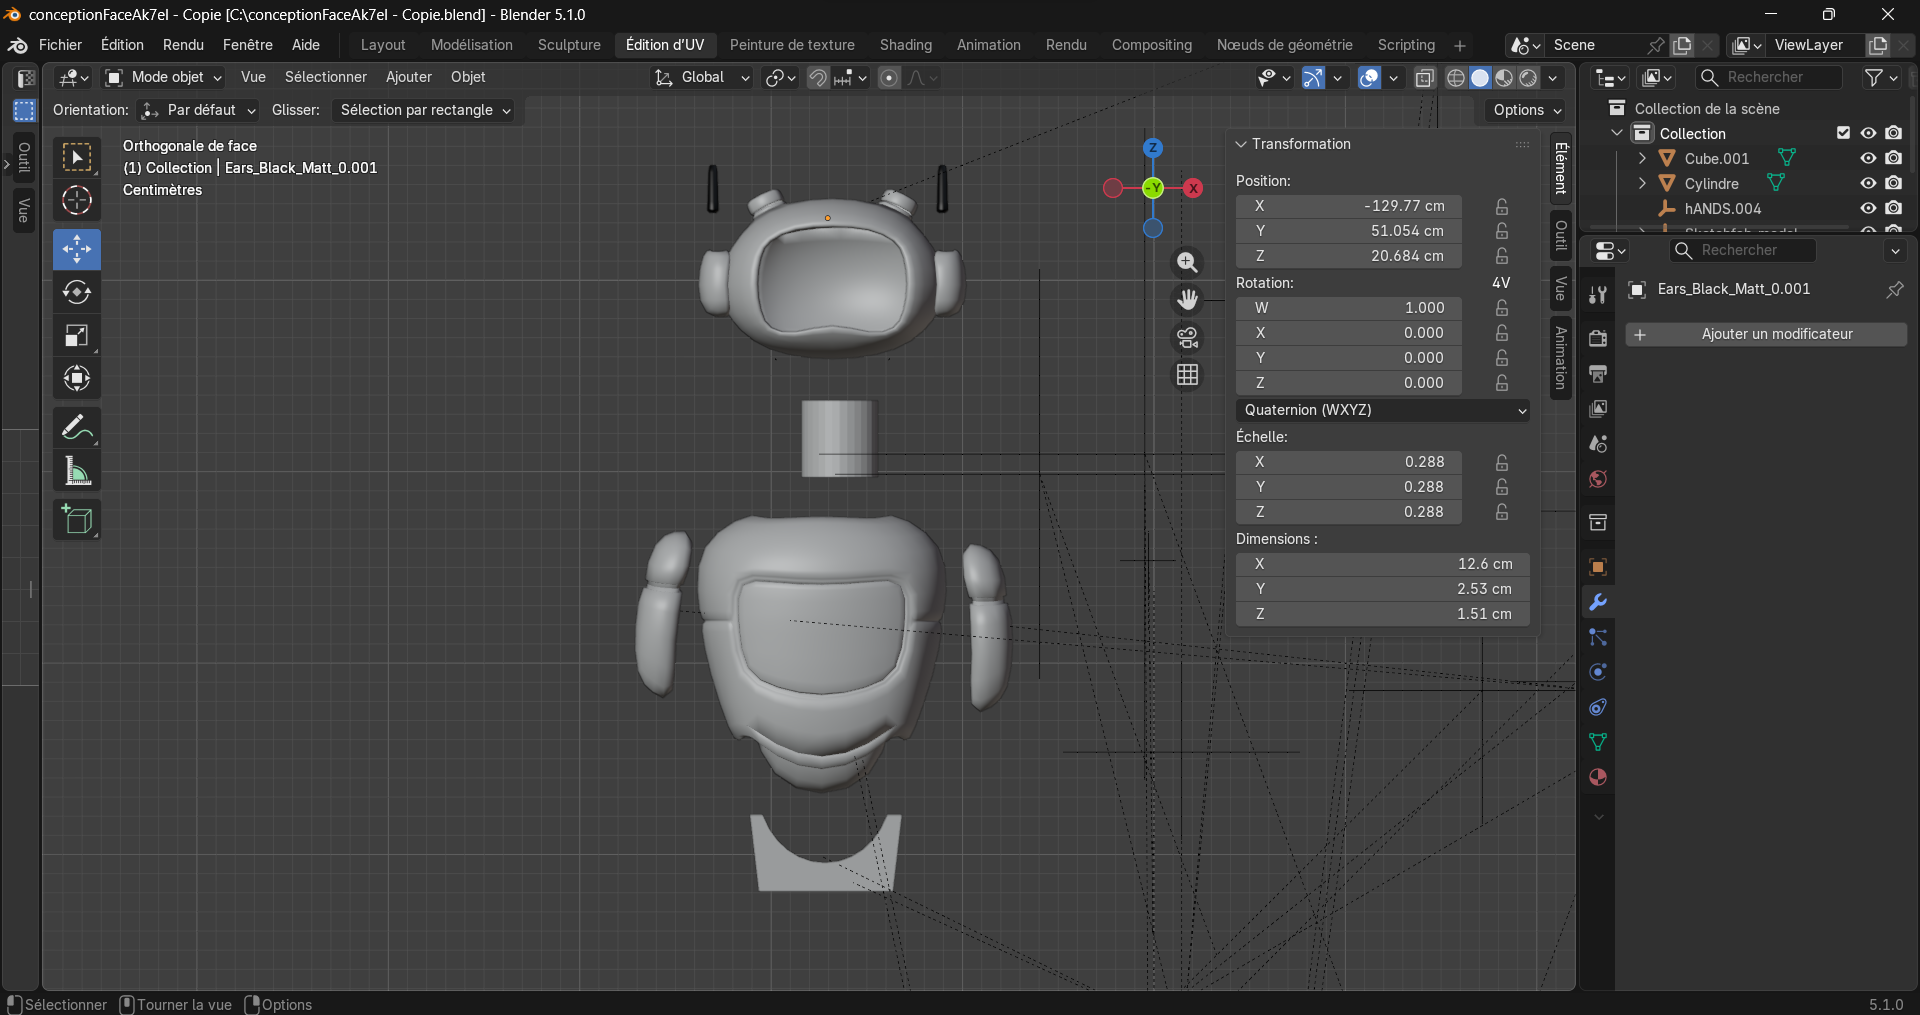
\includegraphics[width=0.92\textwidth]{public/conception3d.png}
		}{%
			\fbox{\textit{Figure manquante~: \texttt{public/conception3d.png}}}
		}
		\caption{Conception 3D du châssis KODA sous Blender (vue éclatée des pièces)}
		\label{fig:ch3-conception3d}
	\end{figure}
	
	\begin{figure}[htbp]
		\centering
		\IfFileExists{public/robot_reel.jpeg}{%
			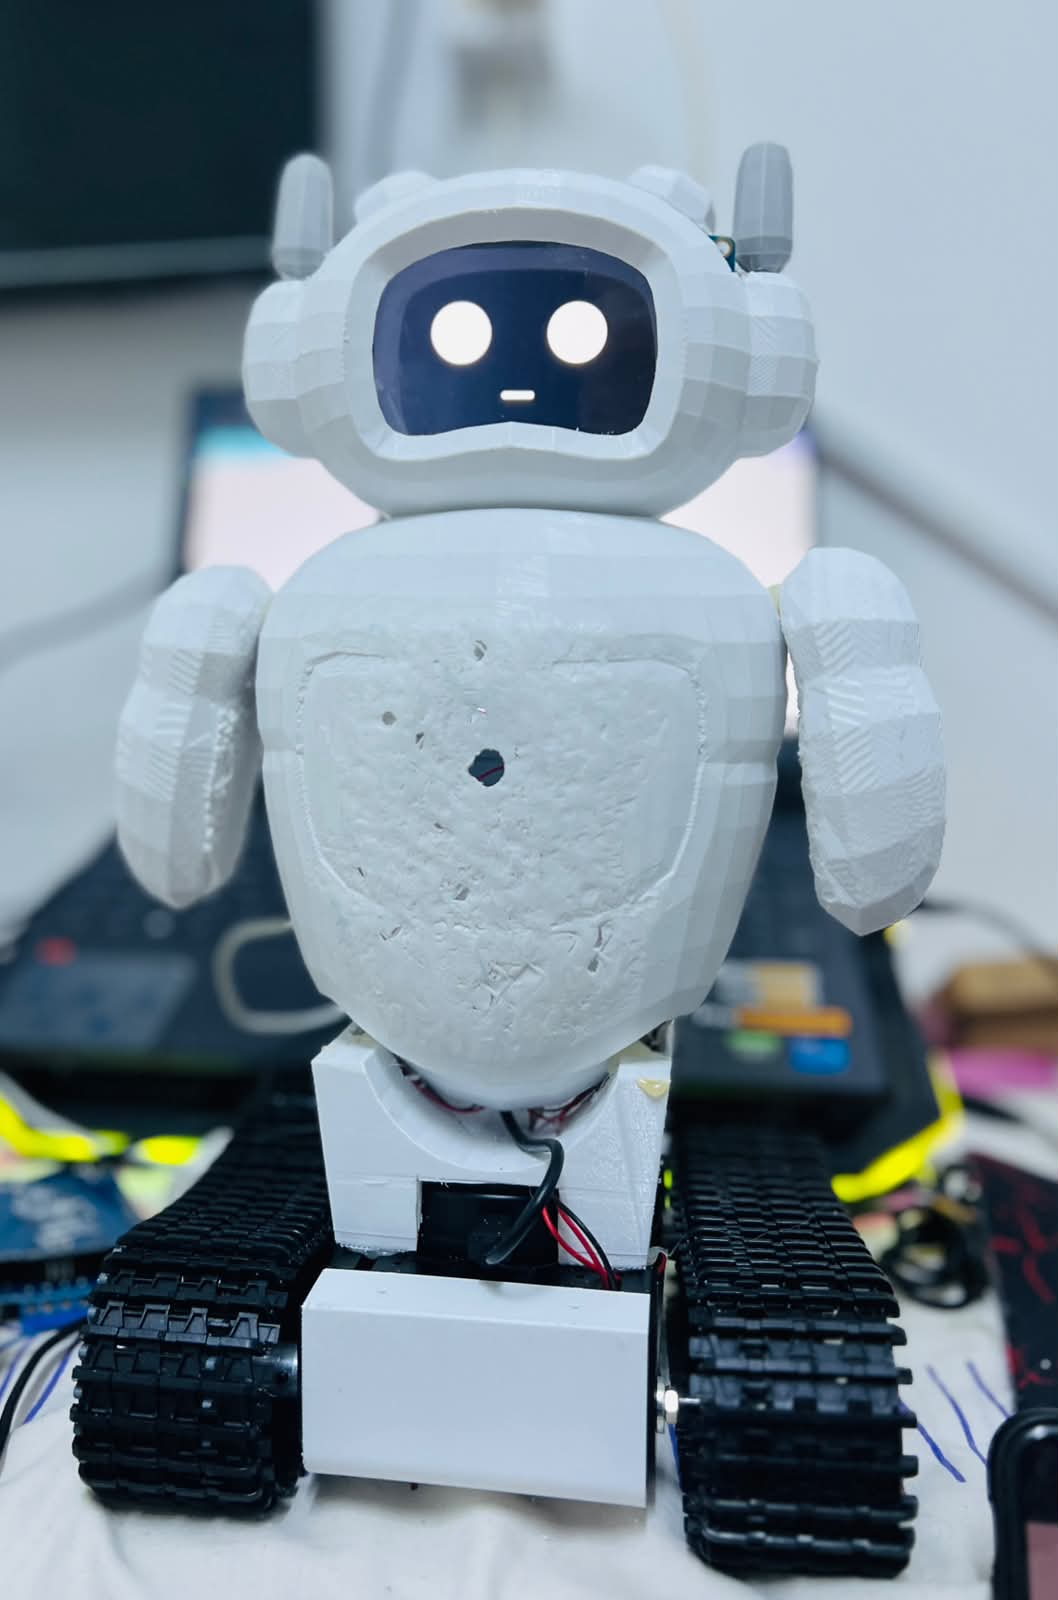
\includegraphics[width=0.75\textwidth]{public/robot_reel.jpeg}
		}{%
			\fbox{\textit{Figure manquante~: \texttt{public/robot\_reel.jpeg}}}
		}
		\caption{Prototype physique KODA après impression 3D et montage}
		\label{fig:ch3-robot-reel}
	\end{figure}
	
	%------------------------------------------------------------------
	\section{Description Détaillée des Composants}
	%------------------------------------------------------------------
	
	%--- Raspberry Pi ---
	\subsection{Unité Centrale~: Raspberry Pi 4 Model B}
	
	Le \textbf{Raspberry Pi 4 Model B} constitue le cœur du robot KODA. Il s'agit
	d'un ordinateur monocarte (SBC — \textit{Single Board Computer}) basé sur un
	processeur ARM Cortex-A72 quadricœur cadencé à 1{,}5~GHz, équipé de 4~Go
	de mémoire RAM LPDDR4.
	
	Dans l'architecture de KODA, le Raspberry Pi assure les fonctions suivantes~:
	\begin{itemize}
		\item \textbf{Communication réseau}~: connexion Wi-Fi au backend (Distributeur
		de Services) pour l'échange de données avec les workflows n8n et la base
		de données.
		\item \textbf{Traitement audio}~: ReSpeaker en entrée (USB) ; sortie soit
		via le \textbf{jack 3{,}5~mm} et l'amplificateur PAM8403, soit via
		\textbf{Bluetooth} vers un haut-parleur externe.
		\item \textbf{Traitement vidéo}~: acquisition d'images via la caméra pour
		la reconnaissance faciale.
		\item \textbf{Pilotage de l'écran Nextion}~: communication série UART pour
		l'affichage des expressions faciales.
		\item \textbf{Commande de l'Arduino}~: envoi d'instructions de mouvement via
		la liaison série USB.
	\end{itemize}
	
	\begin{table}[htbp]
		\centering
		\caption{Spécifications techniques du Raspberry Pi 4 Model B}
		\label{tab:rpi4_specs}
		\renewcommand{\arraystretch}{1.2}
		\begin{tabular}{|l|l|}
			\hline
			\textbf{Caractéristique} & \textbf{Valeur} \\
			\hline
			Processeur & Broadcom BCM2711, Cortex-A72 quad-core @ 1{,}5 GHz \\
			\hline
			Mémoire & 4 Go LPDDR4 \\
			\hline
			Connectivité & Wi-Fi 802.11ac, Bluetooth 5.0 \\
			\hline
			Ports USB & 2$\times$ USB 3.0 + 2$\times$ USB 2.0 \\
			\hline
			Sortie audio & Jack 3{,}5 mm stéréo \\
			\hline
			Interface caméra & Port CSI (Camera Serial Interface) \\
			\hline
			GPIO & 40 broches (dont UART, I2C, SPI) \\
			\hline
			Alimentation & 5V / 3A via USB-C \\
			\hline
		\end{tabular}
	\end{table}
	
	%--- Arduino + L293D ---
	\subsection{Unité de Commande Moteur~: Arduino Uno + Shield L293D}
	
	L'\textbf{Arduino Uno} est une carte de développement à microcontrôleur
	ATmega328P, cadencé à 16~MHz. Il est couplé au \textbf{Shield L293D},
	un circuit intégré de pilotage moteur (\textit{motor driver}) qui permet de
	contrôler simultanément jusqu'à 4~moteurs DC et 2~servomoteurs.
	
	Dans KODA, l'Arduino reçoit ses instructions du Raspberry Pi via une
	\textbf{liaison série USB} et pilote~:
	\begin{itemize}
		\item \textbf{2 moteurs DC} (bornes \textbf{M1} et \textbf{M3} du shield)~:
		déplacement par traction différentielle.
		\item \textbf{3 servomoteurs}~:
		\begin{itemize}
			\item \textbf{S1}~: bras droit
			\item \textbf{S2}~: bras gauche
			\item \textbf{S3}~: tête / cou (rotation de l'écran Nextion uniquement)
		\end{itemize}
	\end{itemize}
	
	Le Shield L293D est alimenté indépendamment par \textbf{3~piles lithium
	de 3{,}7~V} connectées en série, fournissant une tension nominale d'environ
	11{,}1~V nécessaire au fonctionnement des moteurs DC sous charge.
	
	%--- Actionneurs ---
	\subsection{Système d'Actionneurs}
	
	\subsubsection{Moteurs DC --- Mobilité}
	
	Les deux moteurs à courant continu assurent la \textbf{locomotion} du robot
	par un système de \textbf{traction différentielle}~: en faisant varier
	indépendamment la vitesse et le sens de rotation de chaque moteur, le robot
	peut avancer, reculer, tourner à gauche ou à droite. Ce principe simple
	et éprouvé est largement utilisé en robotique mobile (figure~\ref{fig:ch3-traction-diff}).
	
	\begin{figure}[htbp]
		\centering
		\IfFileExists{public/ch3-traction-differentielle.png}{%
			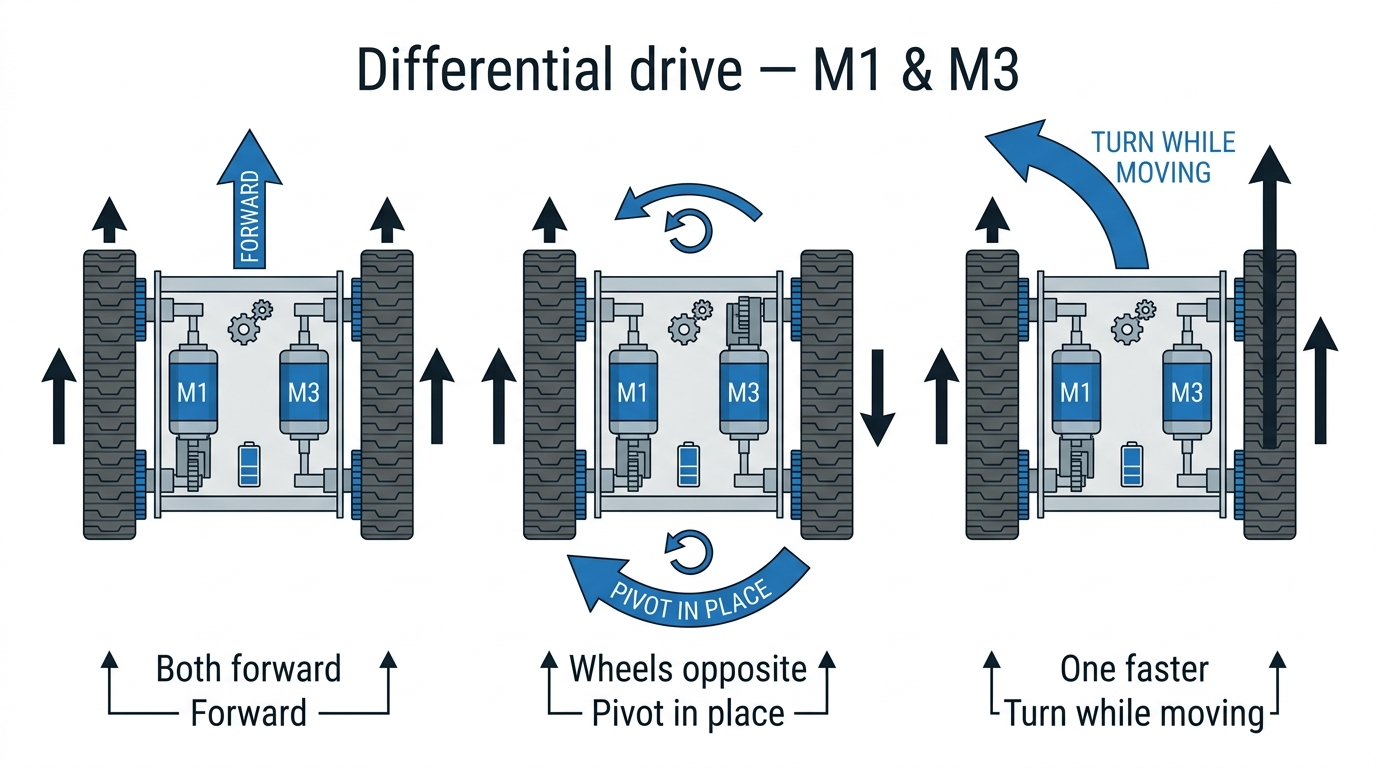
\includegraphics[width=0.85\textwidth]{public/ch3-traction-differentielle.png}
		}{%
			\fbox{\begin{minipage}{0.85\textwidth}\centering\vspace{0.8cm}
				\textit{Figure à ajouter~: \texttt{public/ch3-traction-differentielle.png}}
			\vspace{0.8cm}\end{minipage}}
		}
		\caption{Principe de traction différentielle — moteurs M1 et M3}
		\label{fig:ch3-traction-diff}
	\end{figure}
	
	\subsubsection{Servomoteurs --- Articulations}
	
	Les trois servomoteurs offrent à KODA des capacités d'\textbf{expression
	corporelle}~:
	\begin{itemize}
		\item \textbf{Servomoteur S1 (bras droit)} et \textbf{S2 (bras gauche)}~:
		permettent de simuler des gestes d'accueil, de salutation ou d'indication
		directionnelle.
		\item \textbf{Servomoteur S3 (tête / cou)}~: oriente uniquement
		l'\textbf{écran Nextion} (visage animé). La \textbf{caméra} est fixée sur le
		\textbf{châssis} (corps) du robot et ne suit pas ce mouvement.
	\end{itemize}
	
	%--- Audio ---
	\subsection{Système Audio}
	
	\subsubsection{Entrée Audio~: ReSpeaker 4-Mic Array USB}
	
	Le \textbf{ReSpeaker 4-Mic Array} de Seeed Studio est un périphérique USB
	intégrant quatre microphones MEMS disposés en configuration circulaire.
	Cette disposition permet deux fonctionnalités essentielles~:
	\begin{itemize}
		\item \textbf{Capture vocale omnidirectionnelle}~: enregistrement de la voix
		de l'utilisateur quelle que soit sa position autour du robot.
		\item \textbf{Détection de la Direction d'Arrivée (DOA ---
		\textit{Direction of Arrival})}~: identification de l'angle d'où provient
		la voix. Le robot \textbf{pivote sur place} grâce aux \textbf{deux moteurs DC}
		(M1, M3) pour s'orienter vers l'interlocuteur, puis la \textbf{caméra}
		(fixée sur le corps) permet la détection du visage
		(figure~\ref{fig:ch3-schema-doa}).
	\end{itemize}
	
	\begin{figure}[htbp]
		\centering
		\IfFileExists{public/ch3-schema-doa.png}{%
			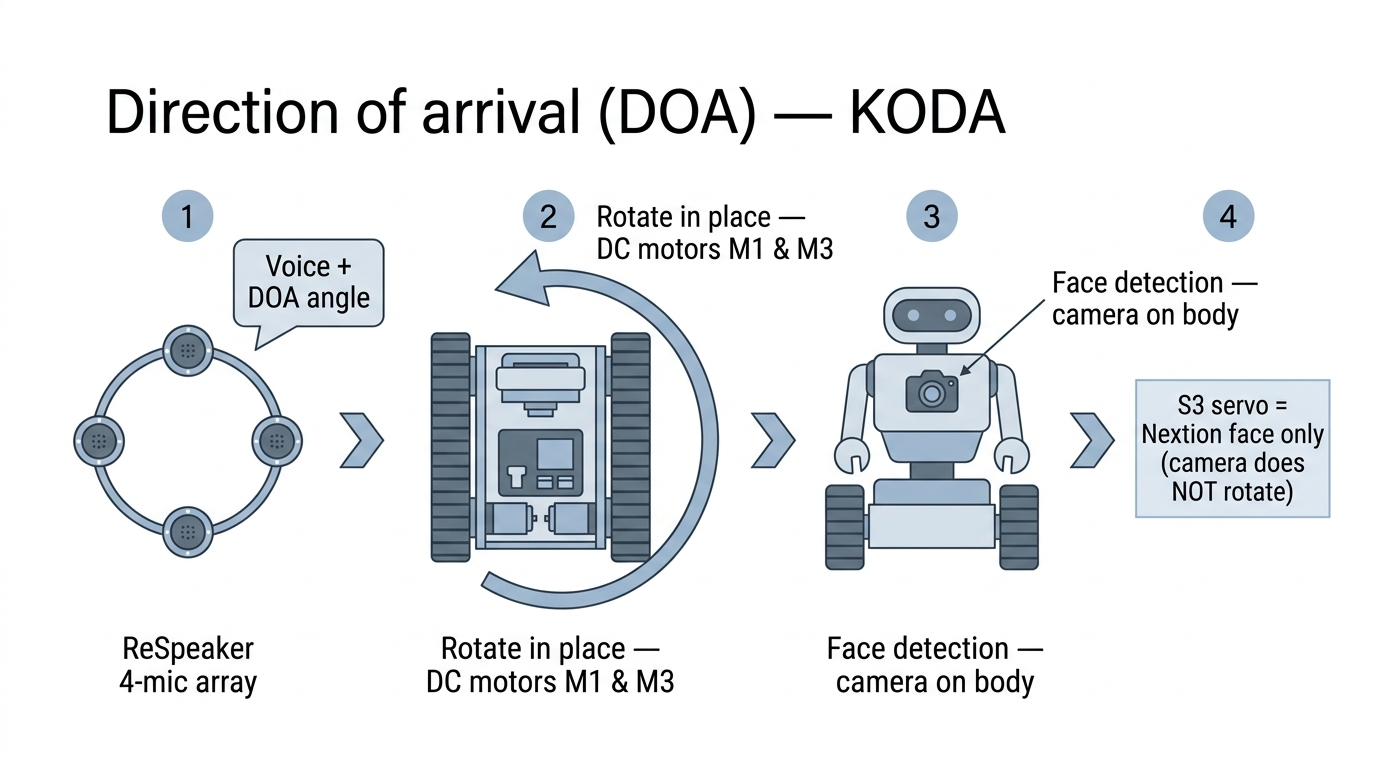
\includegraphics[width=0.88\textwidth]{public/ch3-schema-doa.png}
		}{%
			\fbox{\begin{minipage}{0.88\textwidth}\centering\vspace{0.8cm}
				\textit{Figure à ajouter~: \texttt{public/ch3-schema-doa.png}}
			\vspace{0.8cm}\end{minipage}}
		}
		\caption{Enchaînement conceptuel~: DOA (micro) $\rightarrow$ rotation du robot (M1, M3) $\rightarrow$ caméra (torse)}
		\label{fig:ch3-schema-doa}
	\end{figure}
	
	Le ReSpeaker est connecté au Raspberry Pi via un \textbf{port USB} et est
	reconnu comme un périphérique audio standard sous Linux.
	
	\subsubsection{Sortie Audio~: double chaîne (jack filaire et Bluetooth)}
	
	KODA dispose de \textbf{deux modes de restitution} de la parole, tous deux
	pilotés depuis le Raspberry Pi~:
	
	\begin{itemize}
		\item \textbf{Chaîne filaire}~: sortie \textbf{jack 3{,}5~mm} du Pi
		$\rightarrow$ amplificateur \textbf{PAM8403} $\rightarrow$ deux
		haut-parleurs (gauche / droite). Solution compacte, intégrée au châssis.
		\item \textbf{Chaîne sans fil}~: le Bluetooth intégré du Raspberry Pi~4
		peut envoyer le flux audio vers un \textbf{haut-parleur Bluetooth}
		(appairage classique). Utile pour les essais ou une sortie plus puissante
		sans modifier le câblage jack.
	\end{itemize}
	
	Le choix entre les deux dépend du contexte de démonstration~; la couche
	logicielle (Cycle~4) sélectionnera la carte audio ALSA appropriée.
	
	%--- Vision ---
	\subsection{Système de Vision~: Caméra Raspberry Pi}
	
	La \textbf{caméra officielle Raspberry Pi} est connectée via le port
	\textbf{CSI} (nappe dédiée). Elle fournit les images nécessaires à
	l'\textbf{identification visuelle} des utilisateurs.
	
	Au niveau matériel, seule la \textbf{qualité de capture} (netteté,
	éclairage, cadrage) est concernée dans ce cycle. L'envoi des images vers
	le serveur distant et le traitement logiciel seront détaillés au
	\textbf{Cycle~4}.
	
	%--- Nextion ---
	\subsection{Interface d'Expression Faciale~: Nextion NX4832T035\_011}
	
	L'écran \textbf{Nextion NX4832T035\_011} (3{,}5 pouces) intègre son propre
	microcontrôleur~: le Raspberry Pi n'affiche pas des pixels en temps réel,
	mais envoie des \textbf{commandes série} pour changer de page ou d'expression
	(sourire, surprise, écoute, etc.) déjà stockées dans la mémoire de l'écran.
	
	\textbf{Alimentation et liaison} (câblage retenu sur le prototype)~:
	\begin{itemize}
		\item \textbf{5\,V} et \textbf{GND} du Nextion reliés au \textbf{5\,V}
		et \textbf{GND} du GPIO du Raspberry Pi (masse commune).
		\item \textbf{RX} du Nextion (fil jaune) $\rightarrow$ broche \textbf{8}
		du Pi (\textbf{GPIO~14}, ligne \textbf{TX} du Pi).
		\item \textbf{TX} du Nextion (fil bleu) $\rightarrow$ broche \textbf{10}
		du Pi (\textbf{GPIO~15}, ligne \textbf{RX} du Pi).
	\end{itemize}
	
	Ce câblage UART permet au Pi d'animer le \textbf{visage} de KODA sans
	surcharger le bus USB, tout en gardant une interface visuelle dédiée à
	l'interaction humaine.
	
	%--- Alimentation ---
	\subsection{Système d'Alimentation}
	
	Le robot KODA dispose de \textbf{deux sources d'alimentation indépendantes},
	séparant volontairement la partie logique de la partie motrice~:
	
	\begin{table}[htbp]
		\centering
		\caption{Architecture d'alimentation de KODA}
		\label{tab:alimentation}
		\renewcommand{\arraystretch}{1.25}
		\begin{tabular}{|p{3.5cm}|p{3.5cm}|p{6cm}|}
			\hline
			\textbf{Source} & \textbf{Caractéristiques} & \textbf{Composants alimentés} \\
			\hline
			Power Bank & 5V / 3A, USB-C & Raspberry Pi 4 (et par extension~: ReSpeaker,
			caméra, écran Nextion via GPIO) \\
			\hline
			3$\times$ piles Li-ion & 3{,}7V chacune (11{,}1V total) &
			Shield L293D, moteurs DC, servomoteurs \\
			\hline
		\end{tabular}
	\end{table}
	
	Cette séparation protège le Raspberry Pi contre les perturbations
	électromagnétiques et les chutes de tension provoquées par les appels
	de courant des moteurs.
	
	%------------------------------------------------------------------
	\section{Schéma de Câblage Global}
	%------------------------------------------------------------------
	
	La figure~\ref{fig:ch3-architecture-materielle} présente le
	\textbf{schéma de montage} du prototype~: vue type \textit{Fritzing},
	avec l'ensemble des connexions entre Raspberry Pi, Arduino, capteurs,
	actionneurs et alimentations.
	
	\begin{figure}[htbp]
		\centering
		\IfFileExists{public/ch3-architecture-materielle.png}{%
			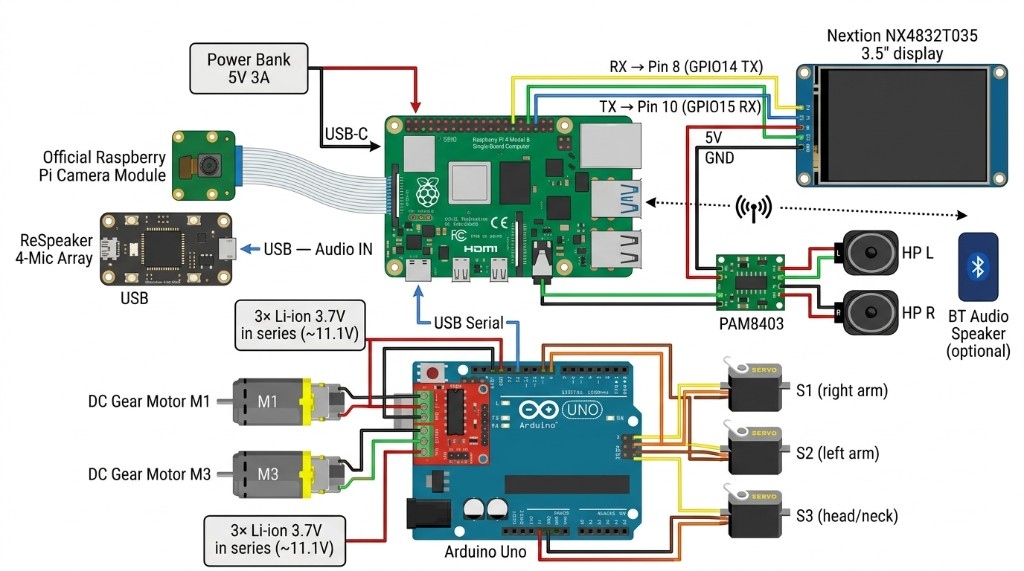
\includegraphics[width=\textwidth]{public/ch3-architecture-materielle.png}
		}{%
			\fbox{\begin{minipage}{0.88\textwidth}\centering\vspace{1.2cm}
				\textit{Figure manquante~: \texttt{public/ch3-architecture-materielle.png}}
			\vspace{1.2cm}\end{minipage}}
		}
		\caption{Schéma de montage matériel de KODA — style Fritzing (Cycle~3)}
		\label{fig:ch3-architecture-materielle}
	\end{figure}
	
	Le tableau~\ref{tab:cablage} récapitule les connexions pour la rédaction
	et la maintenance du prototype.
	
	\begin{table}[htbp]
		\centering
		\caption{Récapitulatif des connexions entre composants}
		\label{tab:cablage}
		\renewcommand{\arraystretch}{1.25}
		\begin{tabularx}{\textwidth}{|p{3.2cm}|p{2.8cm}|p{2.2cm}|X|}
			\hline
			\textbf{Composant} & \textbf{Connecté à} & \textbf{Interface} & \textbf{Détail} \\
			\hline
			Arduino Uno & Raspberry Pi & USB & Commandes moteur (série) \\
			\hline
			ReSpeaker 4-Mic & Raspberry Pi & USB & Entrée audio + DOA \\
			\hline
			PAM8403 + HP L/R & Raspberry Pi & Jack 3{,}5~mm & Sortie filaire \\
			\hline
			HP Bluetooth & Raspberry Pi & Bluetooth & Sortie sans fil (option) \\
			\hline
			Caméra Pi & Raspberry Pi & CSI & Nappe caméra \\
			\hline
			Nextion NX4832T035\_011 & Raspberry Pi & UART + alim &
			5V/GND GPIO ; RX$\rightarrow$ pin~8 ; TX$\rightarrow$ pin~10 \\
			\hline
			Moteurs DC M1, M3 & Shield L293D & Bornes M1, M3 & Traction différentielle \\
			\hline
			Servos S1, S2, S3 & Shield L293D & Servo 1, 2, 3 & Bras D/G ; S3 = Nextion \\
			\hline
			Power Bank 5V/3A & Raspberry Pi & USB-C & Alimentation logique \\
			\hline
			3$\times$ piles 3{,}7V (série) & Shield L293D & Vin & Alimentation motrice \\
			\hline
		\end{tabularx}
	\end{table}
	
	%------------------------------------------------------------------
	\section{Assemblage et points d'attention}
	%------------------------------------------------------------------
	
	L'intégration physique a mis en évidence quelques \textbf{contraintes}
	récurrentes, sans entrer dans le détail logiciel (Cycle~4)~:
	\begin{itemize}
		\item \textbf{Séparation des alimentations}~: éviter de nourrir les moteurs
		depuis le 5\,V du Pi~; les perturbations PWM peuvent provoquer des
		réinitialisations ou du bruit sur l'audio.
		\item \textbf{UART Nextion}~: respecter le croisement TX/RX (fil RX de
		l'écran vers TX du Pi) et une masse commune stable.
		\item \textbf{USB multiples}~: ReSpeaker, Arduino et alimentation
		compétent pour les ports USB du Pi~; une alimentation 5\,V/3\,A fiable
		(power bank) est indispensable.
		\item \textbf{Encombrement mécanique}~: la nappe CSI (caméra sur le corps)
		et les câbles des servos (dont S3 pour le Nextion) doivent rester libres
		de frottement lors des mouvements articulés.
	\end{itemize}
	
	%------------------------------------------------------------------
	\section{Validation matérielle — tests par composant}
	%------------------------------------------------------------------
	
	Chaque sous-système a été validé \textbf{individuellement} avant le test
	global (contrôle visuel ou fonctionnel, sans détailler les scripts).
	Le tableau~\ref{tab:tests_unitaires_cycle3} ci-dessous synthétise cette
	démarche.
	
	\begin{table}[htbp]
		\centering
		\caption{Tests unitaires par composant (Cycle~3)}
		\label{tab:tests_unitaires_cycle3}
		\renewcommand{\arraystretch}{1.35}
		\small
		\begin{tabularx}{\textwidth}{|>{\raggedright\arraybackslash}p{2.6cm}|>{\raggedright\arraybackslash}X|>{\raggedright\arraybackslash}p{3.2cm}|}
			\hline
			\textbf{Composant} & \textbf{Procédure (concept)} & \textbf{Critère OK} \\
			\hline
			Power Bank + Pi & Mise sous tension, boot Raspberry Pi OS &
			LED activité, pas de brown-out \\
			\hline
			ReSpeaker USB & Enregistrement court, niveau sonore &
			Signal audible, périphérique reconnu \\
			\hline
			Sortie jack + PAM8403 & Lecture d'un son test sur les HP &
			Son clair L/R \\
			\hline
			Sortie Bluetooth & Appairage HP BT, lecture test &
			Son sur HP externe \\
			\hline
			Caméra CSI & Capture d'une image fixe &
			Image nette, pas de bandes \\
			\hline
			Nextion UART & Changement de page ou d'expression &
			Affichage réactif \\
			\hline
			Arduino + USB & Envoi d'une commande simple (moniteur série) &
			Réponse attendue \\
			\hline
			Moteurs M1, M3 & Avancer, reculer, pivoter &
			Roues cohérentes \\
			\hline
			Servos S1, S2, S3 & Balayage angle min--max &
			Mouvement fluide, sans à-coups \\
			\hline
			Alim.\ 3 piles (série) & Charge moteurs à vide &
			Tension stable sur Vin \\
			\hline
		\end{tabularx}
		\normalsize
	\end{table}
	
	\subsection{Test d'intégration matérielle}
	
	Le \textbf{test complet} consiste à alimenter l'ensemble, vérifier que le Pi
	détecte simultanément micro, caméra et écran, que l'Arduino répond toujours
	sur USB, et qu'un scénario court combine~: capture vocale, mouvement des
	servos, rotation des roues, changement d'expression Nextion, sans coupure
	d'alimentation ni conflit USB. Ce test valide la \textbf{plateforme prête
	pour le Cycle~4} (logiciel embarqué et liaison réseau avec le backend).
	
	%------------------------------------------------------------------
	\section{Conclusion}
	%------------------------------------------------------------------
	
	Ce chapitre a présenté l'intégralité de la plateforme matérielle du robot
	KODA. L'architecture biprocesseur retenue — Raspberry Pi pour l'intelligence
	et l'Arduino pour le contrôle moteur — garantit à la fois la puissance de
	calcul nécessaire aux traitements IA et la précision temporelle requise
	pour le pilotage des actionneurs.
	
	Chaque composant a été sélectionné et intégré pour répondre aux exigences
	fonctionnelles définies au chapitre~II~: mobilité, interaction vocale
	bidirectionnelle, reconnaissance visuelle et expression émotionnelle.
	La plateforme matérielle est désormais prête à accueillir la couche logicielle
	embarquée, objet du \textbf{Cycle~4} présenté dans le chapitre suivant.
	
	\begin{tcolorbox}[colback=blue!5!white, colframe=blue!60!black,
		title=\textbf{Points clés du Cycle 3}]
		\begin{itemize}[noitemsep]
			\item Architecture biprocesseur~: Raspberry Pi 4 + Arduino Uno / L293D
			\item 5 actionneurs~: M1/M3 (DC) + S1/S2 (bras) + S3 (Nextion)
			\item Audio~: ReSpeaker (entrée) ; sortie jack/PAM8403 ou Bluetooth
			\item Nextion NX4832T035\_011 (UART GPIO 8/10, alim. 5\,V Pi)
			\item Tests unitaires puis intégration~; logiciel au Cycle~4
		\end{itemize}
	\end{tcolorbox}

\end{document}
